% Generated fragments require trusted human review before compilation.
% This binder never requests shell escape or runs external tools.
\documentclass[11pt]{article}
% Trusted shared apparatus. Requires LuaLaTeX; never use shell escape.
\usepackage{fontspec}
\defaultfontfeatures{Ligatures=TeX}
\IfFontExistsTF{Noto Serif}{\setmainfont{Noto Serif}}{%
  \IfFontExistsTF{DejaVu Serif}{\setmainfont{DejaVu Serif}}{%
    \IfFontExistsTF{Times New Roman}{\setmainfont{Times New Roman}}{%
      \PackageError{gelfand-binder}{No configured Cyrillic serif font installed}{Install Noto Serif or DejaVu Serif, or select an installed Cyrillic font.}%
    }%
  }%
}
\IfFontExistsTF{Noto Sans}{\setsansfont{Noto Sans}}{%
  \IfFontExistsTF{DejaVu Sans}{\setsansfont{DejaVu Sans}}{\setsansfont{Arial}}%
}
\IfFontExistsTF{Noto Sans Mono}{\setmonofont{Noto Sans Mono}}{%
  \IfFontExistsTF{DejaVu Sans Mono}{\setmonofont{DejaVu Sans Mono}}{\setmonofont{Courier New}}%
}
\usepackage[a4paper,margin=22mm]{geometry}
\usepackage{amsmath,amssymb,amsthm,mathtools}
\usepackage{xcolor}
\usepackage{tikz}
\usepackage{tikz-cd}
\usetikzlibrary{arrows.meta,positioning,calc}
\usepackage{hyperref}
\hypersetup{unicode=true,colorlinks=true,linkcolor=blue,pdftitle={Gelfand transcription binder}}
\newtheorem{theorem}{Theorem}
\newtheorem{lemma}{Lemma}
\newtheorem{proposition}{Proposition}
\newtheorem{corollary}{Corollary}
\theoremstyle{definition}
\newtheorem{definition}{Definition}
\newtheorem{example}{Example}
\theoremstyle{remark}
\newtheorem{remark}{Remark}
\setlength{\parindent}{0pt}
\setlength{\parskip}{0.55em}
\setlength{\emergencystretch}{3em}
\newcommand{\SourcePage}[2]{%
  \clearpage\phantomsection\label{#1:source-page}%
  \addcontentsline{toc}{subsection}{#1}%
  {\small\sffamily\color{blue!60!black}Source scan frame: #1; visible page/leaf label: #2}\par\medskip%
}
\newcommand{\Unclear}[3]{%
  \begingroup\color{orange!70!black}%
  [Unresolved reading #1/#2: #3]\endgroup%
}
\newcommand{\Incomplete}[3]{%
  \par\begingroup\color{red!65!black}\textbf{Incomplete #1/#2:} #3\endgroup\par%
}
\newcommand{\SourceFigure}[3]{%
  \par\begingroup\color{blue!60!black}\textbf{\hyperref[#1:source-page]{Source figure #1/#2}:} #3%
  \par\textit{Consult the authoritative scan at this locator.}\endgroup\par%
}



% Reader layout only. Original diplomatic text is retained verbatim.
\setlength{\parskip}{0.35em}
\setlength{\emergencystretch}{4em}
\renewcommand{\SourcePage}[2]{%
  \par\addvspace{1em}\phantomsection\label{#1:source-page}%
  \addcontentsline{toc}{subsection}{#1}%
  {\footnotesize\sffamily\color{blue!55!black}#1%
    \def\givenlabel{#2}\def\nolabel{unlabelled}%
    \ifx\givenlabel\nolabel\else\quad[номер в источнике: #2]\fi
  }\par\nobreak\smallskip%
}
\renewcommand{\Unclear}[3]{%
  \begingroup\color{orange!65!black}%
  \ifmmode\text{[неясно: #3]}\else[неясно: #3]\fi\endgroup%
}
\renewcommand{\Incomplete}[3]{%
  \par\begingroup\color{red!60!black}\textbf{Неразобранный фрагмент:} #3%
  \endgroup\par%
}
\renewcommand{\SourceFigure}[3]{%
  \par\begingroup\color{blue!55!black}\textbf{Рисунок:} #3%
  \par{\small\textit{Исходный рисунок: \hyperref[#1:source-page]{#1}, #2.}}%
  \endgroup\par%
}
\hypersetup{pdftitle={Семинар И. М. Гельфанда. Дипломатическая транскрипция},pdfauthor={},pdfsubject={Русское рабочее издание с отмеченными сомнительными чтениями}}

\usepackage[normalem]{ulem}
\usepackage{newunicodechar}
\usepackage{adjustbox}
\newfontfamily\SourceSymbolFont{Segoe UI Symbol}
\newfontfamily\SourceCJKFont{MS Gothic}
\let\DiplomaticMathUnderline\underline
\renewcommand{\underline}[1]{\ifmmode\DiplomaticMathUnderline{#1}\else\uline{#1}\fi}
\newunicodechar{→}{\ifmmode\text{{\SourceSymbolFont\char"2192}}\else{\SourceSymbolFont\char"2192}\fi}
\newunicodechar{⇒}{\ifmmode\text{{\SourceSymbolFont\char"21D2}}\else{\SourceSymbolFont\char"21D2}\fi}
\newunicodechar{∀}{\ifmmode\text{{\SourceSymbolFont\char"2200}}\else{\SourceSymbolFont\char"2200}\fi}
\newunicodechar{∂}{\ifmmode\text{{\SourceSymbolFont\char"2202}}\else{\SourceSymbolFont\char"2202}\fi}
\newunicodechar{∈}{\ifmmode\text{{\SourceSymbolFont\char"2208}}\else{\SourceSymbolFont\char"2208}\fi}
\newunicodechar{∌}{\ifmmode\text{{\SourceSymbolFont\char"220C}}\else{\SourceSymbolFont\char"220C}\fi}
\newunicodechar{√}{\ifmmode\text{{\SourceSymbolFont\char"221A}}\else{\SourceSymbolFont\char"221A}\fi}
\newunicodechar{∞}{\ifmmode\text{{\SourceSymbolFont\char"221E}}\else{\SourceSymbolFont\char"221E}\fi}
\newunicodechar{∧}{\ifmmode\text{{\SourceSymbolFont\char"2227}}\else{\SourceSymbolFont\char"2227}\fi}
\newunicodechar{∩}{\ifmmode\text{{\SourceSymbolFont\char"2229}}\else{\SourceSymbolFont\char"2229}\fi}
\newunicodechar{∪}{\ifmmode\text{{\SourceSymbolFont\char"222A}}\else{\SourceSymbolFont\char"222A}\fi}
\newunicodechar{∫}{\ifmmode\text{{\SourceSymbolFont\char"222B}}\else{\SourceSymbolFont\char"222B}\fi}
\newunicodechar{∴}{\ifmmode\text{{\SourceSymbolFont\char"2234}}\else{\SourceSymbolFont\char"2234}\fi}
\newunicodechar{∼}{\ifmmode\text{{\SourceSymbolFont\char"223C}}\else{\SourceSymbolFont\char"223C}\fi}
\newunicodechar{≈}{\ifmmode\text{{\SourceSymbolFont\char"2248}}\else{\SourceSymbolFont\char"2248}\fi}
\newunicodechar{≠}{\ifmmode\text{{\SourceSymbolFont\char"2260}}\else{\SourceSymbolFont\char"2260}\fi}
\newunicodechar{≤}{\ifmmode\text{{\SourceSymbolFont\char"2264}}\else{\SourceSymbolFont\char"2264}\fi}
\newunicodechar{≥}{\ifmmode\text{{\SourceSymbolFont\char"2265}}\else{\SourceSymbolFont\char"2265}\fi}
\newunicodechar{⊕}{\ifmmode\text{{\SourceSymbolFont\char"2295}}\else{\SourceSymbolFont\char"2295}\fi}
\newunicodechar{⊗}{\ifmmode\text{{\SourceSymbolFont\char"2297}}\else{\SourceSymbolFont\char"2297}\fi}
\newunicodechar{①}{\ifmmode\text{{\SourceSymbolFont\char"2460}}\else{\SourceSymbolFont\char"2460}\fi}
\newunicodechar{②}{\ifmmode\text{{\SourceSymbolFont\char"2461}}\else{\SourceSymbolFont\char"2461}\fi}
\newunicodechar{③}{\ifmmode\text{{\SourceSymbolFont\char"2462}}\else{\SourceSymbolFont\char"2462}\fi}
\newunicodechar{④}{\ifmmode\text{{\SourceSymbolFont\char"2463}}\else{\SourceSymbolFont\char"2463}\fi}
\newunicodechar{Ⓗ}{\ifmmode\text{{\SourceSymbolFont\char"24BD}}\else{\SourceSymbolFont\char"24BD}\fi}
\newunicodechar{〃}{\ifmmode\text{{\SourceCJKFont\char"3003}}\else{\SourceCJKFont\char"3003}\fi}


% Reader revision 3. Annotation wording and candidates remain unchanged.
\setmainfont{NotoSerif-Regular.ttf}[Path=C:/Windows/Fonts/,ItalicFont=NotoSerif-Italic.ttf,BoldFont=NotoSerif-Bold.ttf,BoldItalicFont=NotoSerif-BoldItalic.ttf]
\usetikzlibrary{shapes.geometric,decorations.pathreplacing,decorations.markings,patterns,fit}
\newsavebox{\ReaderAnnotationBox}
\newcommand{\ReaderAnnotation}[1]{%
  \sbox{\ReaderAnnotationBox}{[неясно: #1]}%
  \ifdim\wd\ReaderAnnotationBox>.70\linewidth
    \parbox[t]{.70\linewidth}{\raggedright[неясно: #1]}%
  \else\usebox{\ReaderAnnotationBox}\fi%
}
\ExplSyntaxOn
\cs_new_protected:Npn \reader_unclear_candidate:n #1
 {
  \tl_set:Nx \l_tmpa_tl { \tl_to_str:n {#1} }
  % Text explicitly guarded inside a mathematical candidate remains math-safe.
  \regex_replace_all:nnN { \\(?:text|textrm|textnormal|textbf|operatorname)\s*\{[^{}]*\} } { } \l_tmpa_tl
  \regex_match:nVTF { [\x{0400}-\x{052F}] | \$ } \l_tmpa_tl
   { \ifmmode \text{\ReaderAnnotation{#1}} \else \ReaderAnnotation{#1} \fi }
   {
    \ifmmode
      [\text{неясно:~}#1]
    \else
      \regex_match:nVTF { [_^] | \\ } \l_tmpa_tl
       { \ensuremath{[\text{неясно:~}#1]} }
       { \ReaderAnnotation{#1} }
    \fi
   }
 }
\RenewDocumentCommand \Unclear { m m m }
 { \begingroup\color{orange!65!black}\reader_unclear_candidate:n{#3}\endgroup }
\ExplSyntaxOff
\newsavebox{\ReaderIncompleteBox}
\newcommand{\ReaderIncompleteNote}[1]{%
 \sbox{\ReaderIncompleteBox}{\textbf{Неразобранный фрагмент:} #1}%
 \ifdim\wd\ReaderIncompleteBox>.70\linewidth
  \parbox[t]{.70\linewidth}{\raggedright\textbf{Неразобранный фрагмент:} #1}%
 \else\usebox{\ReaderIncompleteBox}\fi%
}
\renewcommand{\Incomplete}[3]{%
 \ifmmode\text{\color{red!60!black}\ReaderIncompleteNote{#3}}%
 \else\leavevmode\begingroup\color{red!60!black}\ReaderIncompleteNote{#3}\endgroup\fi%
}
% Ragged right avoids stretching long untranslated abbreviations into margins.
\AtBeginDocument{\raggedright}
\newunicodechar{А}{\ifmmode\text{\char"410\relax}\else\char"410\relax\fi}
\newunicodechar{Б}{\ifmmode\text{\char"411\relax}\else\char"411\relax\fi}
\newunicodechar{В}{\ifmmode\text{\char"412\relax}\else\char"412\relax\fi}
\newunicodechar{Г}{\ifmmode\text{\char"413\relax}\else\char"413\relax\fi}
\newunicodechar{Д}{\ifmmode\text{\char"414\relax}\else\char"414\relax\fi}
\newunicodechar{Е}{\ifmmode\text{\char"415\relax}\else\char"415\relax\fi}
\newunicodechar{Ж}{\ifmmode\text{\char"416\relax}\else\char"416\relax\fi}
\newunicodechar{З}{\ifmmode\text{\char"417\relax}\else\char"417\relax\fi}
\newunicodechar{И}{\ifmmode\text{\char"418\relax}\else\char"418\relax\fi}
\newunicodechar{Й}{\ifmmode\text{\char"419\relax}\else\char"419\relax\fi}
\newunicodechar{К}{\ifmmode\text{\char"41A\relax}\else\char"41A\relax\fi}
\newunicodechar{Л}{\ifmmode\text{\char"41B\relax}\else\char"41B\relax\fi}
\newunicodechar{М}{\ifmmode\text{\char"41C\relax}\else\char"41C\relax\fi}
\newunicodechar{Н}{\ifmmode\text{\char"41D\relax}\else\char"41D\relax\fi}
\newunicodechar{О}{\ifmmode\text{\char"41E\relax}\else\char"41E\relax\fi}
\newunicodechar{П}{\ifmmode\text{\char"41F\relax}\else\char"41F\relax\fi}
\newunicodechar{Р}{\ifmmode\text{\char"420\relax}\else\char"420\relax\fi}
\newunicodechar{С}{\ifmmode\text{\char"421\relax}\else\char"421\relax\fi}
\newunicodechar{Т}{\ifmmode\text{\char"422\relax}\else\char"422\relax\fi}
\newunicodechar{У}{\ifmmode\text{\char"423\relax}\else\char"423\relax\fi}
\newunicodechar{Ф}{\ifmmode\text{\char"424\relax}\else\char"424\relax\fi}
\newunicodechar{Х}{\ifmmode\text{\char"425\relax}\else\char"425\relax\fi}
\newunicodechar{Ц}{\ifmmode\text{\char"426\relax}\else\char"426\relax\fi}
\newunicodechar{Ч}{\ifmmode\text{\char"427\relax}\else\char"427\relax\fi}
\newunicodechar{Ш}{\ifmmode\text{\char"428\relax}\else\char"428\relax\fi}
\newunicodechar{Щ}{\ifmmode\text{\char"429\relax}\else\char"429\relax\fi}
\newunicodechar{Ъ}{\ifmmode\text{\char"42A\relax}\else\char"42A\relax\fi}
\newunicodechar{Ы}{\ifmmode\text{\char"42B\relax}\else\char"42B\relax\fi}
\newunicodechar{Ь}{\ifmmode\text{\char"42C\relax}\else\char"42C\relax\fi}
\newunicodechar{Э}{\ifmmode\text{\char"42D\relax}\else\char"42D\relax\fi}
\newunicodechar{Ю}{\ifmmode\text{\char"42E\relax}\else\char"42E\relax\fi}
\newunicodechar{Я}{\ifmmode\text{\char"42F\relax}\else\char"42F\relax\fi}
\newunicodechar{а}{\ifmmode\text{\char"430\relax}\else\char"430\relax\fi}
\newunicodechar{б}{\ifmmode\text{\char"431\relax}\else\char"431\relax\fi}
\newunicodechar{в}{\ifmmode\text{\char"432\relax}\else\char"432\relax\fi}
\newunicodechar{г}{\ifmmode\text{\char"433\relax}\else\char"433\relax\fi}
\newunicodechar{д}{\ifmmode\text{\char"434\relax}\else\char"434\relax\fi}
\newunicodechar{е}{\ifmmode\text{\char"435\relax}\else\char"435\relax\fi}
\newunicodechar{ж}{\ifmmode\text{\char"436\relax}\else\char"436\relax\fi}
\newunicodechar{з}{\ifmmode\text{\char"437\relax}\else\char"437\relax\fi}
\newunicodechar{и}{\ifmmode\text{\char"438\relax}\else\char"438\relax\fi}
\newunicodechar{й}{\ifmmode\text{\char"439\relax}\else\char"439\relax\fi}
\newunicodechar{к}{\ifmmode\text{\char"43A\relax}\else\char"43A\relax\fi}
\newunicodechar{л}{\ifmmode\text{\char"43B\relax}\else\char"43B\relax\fi}
\newunicodechar{м}{\ifmmode\text{\char"43C\relax}\else\char"43C\relax\fi}
\newunicodechar{н}{\ifmmode\text{\char"43D\relax}\else\char"43D\relax\fi}
\newunicodechar{о}{\ifmmode\text{\char"43E\relax}\else\char"43E\relax\fi}
\newunicodechar{п}{\ifmmode\text{\char"43F\relax}\else\char"43F\relax\fi}
\newunicodechar{р}{\ifmmode\text{\char"440\relax}\else\char"440\relax\fi}
\newunicodechar{с}{\ifmmode\text{\char"441\relax}\else\char"441\relax\fi}
\newunicodechar{т}{\ifmmode\text{\char"442\relax}\else\char"442\relax\fi}
\newunicodechar{у}{\ifmmode\text{\char"443\relax}\else\char"443\relax\fi}
\newunicodechar{ф}{\ifmmode\text{\char"444\relax}\else\char"444\relax\fi}
\newunicodechar{х}{\ifmmode\text{\char"445\relax}\else\char"445\relax\fi}
\newunicodechar{ц}{\ifmmode\text{\char"446\relax}\else\char"446\relax\fi}
\newunicodechar{ч}{\ifmmode\text{\char"447\relax}\else\char"447\relax\fi}
\newunicodechar{ш}{\ifmmode\text{\char"448\relax}\else\char"448\relax\fi}
\newunicodechar{щ}{\ifmmode\text{\char"449\relax}\else\char"449\relax\fi}
\newunicodechar{ъ}{\ifmmode\text{\char"44A\relax}\else\char"44A\relax\fi}
\newunicodechar{ы}{\ifmmode\text{\char"44B\relax}\else\char"44B\relax\fi}
\newunicodechar{ь}{\ifmmode\text{\char"44C\relax}\else\char"44C\relax\fi}
\newunicodechar{э}{\ifmmode\text{\char"44D\relax}\else\char"44D\relax\fi}
\newunicodechar{ю}{\ifmmode\text{\char"44E\relax}\else\char"44E\relax\fi}
\newunicodechar{я}{\ifmmode\text{\char"44F\relax}\else\char"44F\relax\fi}
\newunicodechar{Ё}{\ifmmode\text{\char"401\relax}\else\char"401\relax\fi}
\newunicodechar{ё}{\ifmmode\text{\char"451\relax}\else\char"451\relax\fi}

\newunicodechar{æ}{\ifmmode\text{\char"E6\relax}\else\char"E6\relax\fi}
\newunicodechar{−}{\ifmmode\mathbin{\text{\SourceSymbolFont\char"2212\relax}}\else{\SourceSymbolFont\char"2212\relax}\fi}


% Reader-only pairing support; accepted raw bodies remain unchanged.
\RequirePackage{graphicx}
\RequirePackage{adjustbox}
\newcommand{\ReaderOriginalPanel}[2]{%
  \begin{minipage}[t]{.48\linewidth}\vspace{0pt}\centering
    \includegraphics[width=\linewidth,keepaspectratio]{#1}\par\smallskip
    {\scriptsize Оригинал рукописного рисунка: #2}\par
  \end{minipage}%
}
\newcommand{\ReaderDiagramPair}[3]{%
  \par\noindent\begingroup
  \ReaderOriginalPanel{#1}{#2}\hfill
  \begin{minipage}[t]{.48\linewidth}\vspace{0pt}\centering
    {\scriptsize Типографское воссоздание}\par\smallskip
    \begin{adjustbox}{max width=\linewidth}#3\end{adjustbox}\par
  \end{minipage}%
  \endgroup\par\smallskip
}
\newcommand{\ReaderDescriptionPair}[3]{%
  \par\noindent\begingroup
  \ReaderOriginalPanel{#1}{#2}\hfill
  \begin{minipage}[t]{.48\linewidth}\vspace{0pt}\raggedright
    {\scriptsize Типографское описание}\par\smallskip
    #3\par
  \end{minipage}%
  \endgroup\par\smallskip
}


\begin{document}
\begin{center}
{\Large Семинар И. М. Гельфанда}\par\medskip
{\LARGE Дипломатическая транскрипция}\par\bigskip
{\large Рабочее русское издание}\par\medskip
{\large Том 23 из 34. Архивная глава 023}\par\bigskip
Кадры GELFAND-P001074 -- GELFAND-P001132\par
\end{center}
\medskip
Сокращения, отменённые записи и сомнительные чтения сохранены.
Неразобранные фрагменты отмечены в тексте. Математические утверждения
источника переданы без молчаливых исправлений.

В текущем комплекте приняты 165 из 165 возвратов; учтены 1527 из 1527 кадров. Кадров без принятого возврата: 0.
Статусы кадров в отчётах о полноте: транскрибированы 1168, неразборчивы 357, частично прочитаны 1, недоступны 1.
Нерешённых записей журнала чтений: 6820.
Статус «неразборчивый» может отмечать локальную утрату зачёркнутой записи;
он не означает отсутствия всего кадра.
Сверка с рукописью продолжается. Рабочие журналы чтений и происхождения
данных сохранены отдельно.

Ограничения исходного комплекта: повреждённый исходный скан GELFAND-P000722; каталожные записи 603, 694 без сканов; в архивной главе 029 не перечислена часть 25.

Границы кадров показаны небольшими синими указателями; печатный текст
продолжается без обязательного разрыва страницы после каждого кадра.
\bigskip\hrule\bigskip
\SourcePage{GELFAND-P001074}{1}
\underline{7/II-83 г.}

\underline{Сем. Гельфанда}

\underline{И.М.Г.} Нет привычного понимания $\infty$-мерной симплектич. группы,
$\infty$-мерн. [вставлено сверху: симпл.]
\Unclear{GELFAND-P001074}{top-abbreviation}{неразборчиво}
и т.п. «Фоковское пр-во — игрушка для математиков».

Есть попул. лекции Виттена о суперматематике!
(препринт; лекции)
\begin{equation*}
\begin{gathered}
\downarrow\\
\text{Теор. Атья-Ботта получ. из суперобр.}\\
\text{(о неподв. точках)}
\end{gathered}
\end{equation*}

\underline{Кириллов о раб. Неретина}
\begin{equation*}
T(g)f(z)=f\left(\frac{\alpha z+\gamma}{\beta z+\delta}\right)
|\beta z+\delta|^{\lambda}
\end{equation*}
Предст. $SL(2,\mathbb R)$ продолж. до предст.
$\operatorname{Diff}(S^1)$ (унитарно!).
\begin{equation*}
f\longmapsto f(\varphi^{-1}(z))
\left|\frac{d\varphi^{-1}(z)}{dz}\right|^{-\lambda/2}
\end{equation*}
[Приписка слева со скобкой: «это неунитарное, но».]
По этому строятся предст-я унитарные
(из рассм. действия в фок. пр-ве — на
\Unclear{GELFAND-P001074}{coherent-states}{когерент. / когерентных}
состояниях.
[На правом поле, на уровне этого замечания, отдельно стоит «)».]

Идея:
\begin{equation*}
\operatorname{Im}\int f(x_1)\overline{g(x_2)}
\frac{|x_1-x_2|^{-2+\lambda}}{\Gamma(-1+\lambda)}\,dx_1\,dx_2
\qquad\text{(симпл. форма!)}
\end{equation*}
\underline{сохр. при дробно-лин. преобр.}
[Зачёркнуто: \Unclear{GELFAND-P001074}{crossed-arrow}{знак, похожий на стрелку}.]
$\Rightarrow$ при всех диффеом. не сохр., но сим. вид.

\SourceFigure{GELFAND-P001074}{unitary-group-annotation}{Справа: $G=U(1+HS)$.
От $U$ стрелка вниз влево к «унит.», от $HS$ стрелка вниз влево к
«гильб.-шм.». Ниже ещё строка, похожая на «и более общ.»; это не окончательное чтение.
Справа две наклонные черты.}

\underline{Б. Фейгин.}

\underline{Струны и представления $\operatorname{Diff}S^1$.}

$V$ — пр-во отобр. $S^1\longrightarrow\mathbb R^d$,
на $\mathbb R^d$ зад. метрика (рим. или лоренцева).
Действует $\operatorname{Diff}S^1$
(замены пар.).
\begin{equation*}
(1)\qquad f,g\longmapsto\int_{S^1}(f,dg)
\end{equation*}
На $V/V_{\mathrm{const}}$ получ. невырожд. форма;
положим $V'=V/V_{\mathrm{const}}$.
[Под $V_{\mathrm{const}}$: «пост. отобр.».]

На $V'/\operatorname{Diff}S^1$ есть гамильт. структура
(скобка Пуассона).

\underline{Задача:} проквантовать эту ситуацию.
[На правом поле ниже:
\Unclear{GELFAND-P001074}{margin-lower-mark}{короткий наклонный штрих перед закрывающей скобкой}.]

\underline{Кириллов.} $M$ — симпл. мн-во,
$G$ — гр., действ. на $M$ с сохр. симпл. структуры
$\Rightarrow$ строится $M_{\mathrm{red}}$ — редуц. мн-ие
(симплектическая редукция).
Идея: $\{\ \}$ на инвар. ф-ях вырождена; надо профакторизовать.

\underline{Б. Ф.} $V'$ — пр-во с невыр. симпл. формой.
Способ квант. — выбрать $p,q$ и реализ. их обычным образом
(пр-во Фока).
Конечномерн. случай — это удовл. способ. Где действует?
Пр-во инвариантов.
$\infty$-мерный случай — это плохо.
Предст. сим.
\Unclear{GELFAND-P001074}{last-line-subject}{неразборчивое сокращение}
явл. проективным, и инвариантов не существует. Надо менять пр-во.
[Приписка под последней строкой:
\Unclear{GELFAND-P001074}{bottom-parenthesis}{неразборчиво; возможны фрагменты «тип», «павл.»}.]
\Incomplete{GELFAND-P001074}{bottom-parenthesis}{Мелкая приписка в скобках под последней строкой не прочитана целиком.}

\SourcePage{GELFAND-P001075}{unlabelled}
$\operatorname{sp}(V')$ — ал. Ли симпл. преобр.

$\mathcal L$ — ал. вект. полей на $S^1$.

\SourceFigure{GELFAND-P001075}{representation-diagram}{Цепочка
$\mathcal L\longrightarrow\operatorname{sp}(V')\longrightarrow\Phi$.
Над первой стрелкой подпись «Получено предст.» со стрелочкой вниз;
над второй — «Вейль» (чтение не окончательное) со стрелочкой вниз.
Под $\Phi$ вертикальная черта и «фок. пр-во».
Снизу всю цепочку охватывает скобка; к ней направлена стрелка вверх
от подчёркнутой подписи «проект. представл.».}

$\Phi$ строится так:

$V'$,
[зачёркнут знак: \Unclear{GELFAND-P001075}{cancel-after-v}{неразборчиво}]
$S^1\longrightarrow\mathbb R^d$.

комплексифицируем и разложим
\begin{equation*}
\begin{array}{rcccl}
V'={}&H^+&\oplus&H^-&\\
&\vert&&\vert&\\
&\text{(опер. уничт.)}&\leftrightarrow&\text{(опер. рожд.)}&
\end{array}
\qquad
\Phi=\bigoplus S^i H_+.
\end{equation*}
$H^+$ — ф-ии, аналит. внутри.
[Справа от этой строки:
\Unclear{GELFAND-P001075}{faint-right-trace}{бледный прерывистый след; словесное чтение не установлено}.]

\begin{equation*}
\mathcal L=\{L_i,c\},\quad i\in\mathbb Z.
\end{equation*}
\begin{equation*}
[L_i,L_j]=(j-i)L_{i+j}+
\underbrace{\delta_{i,-j}\frac{i^3-i}{12}\,c}_{\text{швингеровский член}}.
\end{equation*}
$\phi^{L_+}$ — пр-во инвар. для подал. $L_+$; есть отобр.
\begin{equation*}
L_+=\{\Unclear{GELFAND-P001075}{cancelled-generator}{\text{зачёркнуто, возможно }L_0},
L_1,L_2,\ldots\},\qquad
L_-=\{L_{-1},L_{-2},\ldots\}.
\end{equation*}
[Справа от этих определений:]
\begin{equation*}
\phi^{L_+}\longrightarrow\Phi/L_-\Phi.
\end{equation*}
[Под стрелкой и её концами общая скобка: «надо взять \underline{образ}».]
\begin{equation*}
\phi^{\mathrm{inv}}=[\operatorname{Im}]^{L_0,\alpha}.
\end{equation*}
[От $\operatorname{Im}$ проведена изогнутая стрелка вправо вверх
к словам «надо взять образ».]

Нетрив. по крайней мере при $\underline{d=26}$.

\underline{Задача} (И.М.Г.). Построить $p$-адич. аналог предст.
группы диффеоморфизмов.

\SourcePage{GELFAND-P001076}{unlabelled}
\underline{14/II-83 г.}\qquad\underline{Сем. Гельфанда.}

\underline{Ю. Неретин.}

$\forall\rho$ почти сохр. скал. произвд.
\begin{equation*}
(1)\qquad \frac{1}{\Gamma(\rho)}\int_{-\infty}^{\infty}
|x_1-x_2|^{-\rho}f(x_1)\overline{g(x_2)}\,dx_1\,dx_2.
\end{equation*}
([Зачёркнуто: \Unclear{GELFAND-P001076}{upper-cancel}{неразборчиво}]
опер. будет $\underline{O(1+T)}$.)
[Под $T$ вертикальная черта к подчёркнутому «Г.Ш.».]

Преобр. Гильберта:
\begin{equation*}
(2)\qquad Hf(s)=\frac{1}{2\pi}\int_0^{2\pi}
\operatorname{ctg}\left(\frac{t-s}{2}\right)f(t)\,dt
\qquad\text{($f$ — вещ. ф-я)}
\end{equation*}
\begin{equation*}
H:\mathrm{const}\longrightarrow0
\end{equation*}
$\rho=0,2\quad\Rightarrow$ в пр-ве, профакториз. по $\mathrm{const}$
или с $\int=0$.

$H$ вводит компл. структуру.

В Фурье:
\begin{equation*}
\begin{aligned}
\cos n\varphi&\longrightarrow-\sin n\varphi\\
\sin n\varphi&\longrightarrow\cos n\varphi
\end{aligned}
\end{equation*}

\underline{Скал. произвд.}
\begin{equation*}
\int\ln\left|\sin\frac{t-s}{2}\right|f_1(t)f_2(s)\,dt\,ds
\end{equation*}
\begin{equation*}
\int\Unclear{GELFAND-P001076}{integrand-cancel}{\text{зачёркнуто, возможно }\ln}
\operatorname{ctg}\left(\frac{t-s}{2}\right)f_1(t)f'_2(s)\,dt\,ds
\end{equation*}
$\Rightarrow$ [зачёркнуто:
\Unclear{GELFAND-P001076}{lower-cancel}{неразборчиво}]
$H$ задаёт компл. структуру.

[Справа: «с пом. разл. на аналит. и антианалит. ф-ии»;
от этой приписки стрелка вниз к следующему замечанию.]
$\Rightarrow$ берём эрмитово продолжение с пом. этого $H$.

$\operatorname{Im}\langle\cdot,\cdot\rangle$
\underline{сохр. при всех диффеоморфизмах}.

\underline{И.М.Г.}\quad\underline{Задача:}
сделать это общим утв. о ПДО!!
(инв. отн. [вставлено сверху: всех] диффеом.!!)

\SourcePage{GELFAND-P001077}{unlabelled}
\underline{Симплектич. форма — ?}

Ю.Н.\quad\underline{Проекторы:}
\Unclear{GELFAND-P001077}{projector-normalization}{$H\pm i$}

образы их: \underline{лагранжевы мн-ия}.

Симпл. форма:
\begin{equation*}
\{f_1,f_2\}=\langle f_1,Hf_2\rangle
\end{equation*}
\underline{И.М.Г.}
[Зачёркнуто: \Unclear{GELFAND-P001077}{cancel-after-img}{неразборчиво}.]
[Вставлено сверху: «Надо ещё».]
рассм. обобщ. $c[1+(\text{комп.})]$
($\Rightarrow$ писать весь ряд в символах).

[Зачёркнутая формула:
\Unclear{GELFAND-P001077}{cancelled-log-kernel}{$\iint\ln\left|\sin\frac{t-s}{2}\right|$}.]

\underline{Утв.}
\begin{equation*}
\iint\ln\left|\frac{t-s}{2}\right|f_1(t)f_2(\sigma)
\frac{1}{s-\sigma}\,ds\,d\sigma\,dt
\end{equation*}
[В знаменателе зачёркнуто
\Unclear{GELFAND-P001077}{corrected-denominator}{$t-\sigma$ / $t-s$};
снизу вписано $s-\sigma$.
Перед $\sigma$ в $d\sigma$ зачёркнут знак:
\Unclear{GELFAND-P001077}{corrected-differential}{$t$ / неразборчиво}.]

\underline{сохраняется при диффеоморфизмах}

$\Rightarrow$ должен быть дифф. оператором ($f'$).

\underline{Надо:} вычислить:
\begin{equation*}
\int\ln\left|\frac{t-s}{2}\right|\frac{1}{s-\sigma}\,ds.
\end{equation*}
Должно получ.
\Unclear{GELFAND-P001077}{delta-prime-claim}{$\delta'$}.

Надо аналит. продолжить!!
\begin{equation*}
\int_{-\infty}^{\infty}|x|^\lambda f(x)\,dx
=\int_{|x|<1}+\int_{|x|>1}
\end{equation*}
[Над двумя интегралами справа и под последним интегралом зачёркнуты пределы:
\Unclear{GELFAND-P001077}{split-integral-limits}{$\infty$, $\infty$, $-\infty$}.]
и продолжаем каждый аналит.

Идея:
\begin{equation*}
\int|t-s|^\lambda\ \ldots
\end{equation*}
\underline{и продиффер. по $\lambda$}!!

[Зачёркнуто: «В. Гинзбург».]
\underline{Ещё зад. (по Фейгину!):}

Как диффеом. $S^1$ действует на послед. аналит. ф-й
\begin{equation*}
\{f_1(z),f_2(z_1,z_{\Unclear{GELFAND-P001077}{f2-second-argument-subscript}{2}}),f_3(z_1,z_2,z_3),\ldots\}
\end{equation*}
$|z|<1$.

Как влияет гладкость?

Для $\varphi$ дробно-линейных это совпадает с обычным!

Как это материализовать?

\SourcePage{GELFAND-P001078}{5}
\underline{В. Гинзбург.}

О раб. \underline{Duistermaat, Heckman}
(Invent. Math., 1982 г.)

$T=\mathbb T^k$ — тор ($k$-мерный);
$M$ — компактное симпл. мн-ие,
$T$ действует на $M$ гамильт. образом:
т.е. сохр. симпл. структуру, и
$\forall$ вект. поле
[зачёркнуто: \Unclear{GELFAND-P001078}{action-cancel}{на / не}]
из ал. Ли $T$ опр. поле,
\Unclear{GELFAND-P001078}{hamiltonian-phrase}{заданное / заданные}
гамильтонианом и эти гамильтонианы
коммутируют (отн. скобки Пуассона).
(Из коммутир. полей не следует коммутир. ф-ий.)
(Сейчас это наз.: пуассоновское гам. действие.)

[Слева, параллельно пояснению о гамильтонианах:]
Возникает отображение:
\SourceFigure{GELFAND-P001078}{moment-map-diagram}{Сверху $M$,
из него стрелка вниз, слева от стрелки $\mu$;
внизу $\xi\in t^*$. Под схемой слабая подпись в скобках:
«отобр. моментов» или «отобр. мом-тов»; окончание неясно.}

Или: зад. ф-и
[над окончанием слова знак:
\Unclear{GELFAND-P001078}{functions-mark}{звёздочка / зачёркнутый знак}]
$f_1,\ldots,f_k$:
$\underline{\{f_i,f_j\}=0}$,
\underline{Потоки $f_i$ периодичны}.

\underline{Локальное условие:}
поля лежат в одном лагранжевом
[зачёркнуто: \Unclear{GELFAND-P001078}{local-cancel}{подпространстве / подпр-ве}]
подпр-ве в $\forall$ точке.

[Зачёркнуто: \Unclear{GELFAND-P001078}{cancelled-heading}{Другое / Далее}.]
\begin{equation*}
(1)\qquad \mu(m)(X)=H_X(m)\qquad\text{($X$ — поле — любое)}
\end{equation*}
Или:
\underline{Коцикл} $X_1,X_2\longrightarrow\omega(X_1,X_2)(m)$
на алгебре Ли должен быть тривиален.

\underline{Пример:} $\{y,-x\}$ зад. коммут. поля
$\dfrac{\partial}{\partial x}$, $\dfrac{\partial}{\partial y}$,
но скобка их $\ne0$.

\begin{equation*}
(2)\qquad M_\xi=\mu^{-1}(\xi);
\quad\text{на нём $\omega$ вырождена;}
\end{equation*}
На $M_\xi/T$ [вставлено сверху: «она»] уже невырождена.
Обозначим её $\omega_\xi$. От неё можно считать объём.

\underline{Утв. леммы:}
$\omega_\xi$ [вставлено сверху: «кус.»] линейно по $\xi$
($\mathrm{mod}$ точных дифф.).

\underline{Следствие.}
\Unclear{GELFAND-P001078}{reduced-volume-notation}{$\operatorname{Vol}(M_\xi)$}
кусочно полиномиален.

(3)\quad\underline{Теорема.} Рассм. вектор $X\in t$
[под $t$: «ал. Ли»] и соотв. гамильтониан $H_X$
(подъём $X$ как ф-и на $t^*$ с пом. $\mu$).
Тогда интеграл
\begin{equation*}
(4)\qquad\int_M e^{iH_X(m)}\,dm
\end{equation*}
(ф-я на алгебре Ли)

можно вычисл. по методу стац. фазы и это даёт точный ответ.

Ответ:
\begin{equation*}
(5)\qquad
\int_M e^{iH_X(m)}\,dm
=\sum_j\frac{\operatorname{vol}(M_j)e^{iH_X(M_j)}}
{\prod_k\lambda_{jk}(X)}
\end{equation*}
\Unclear{GELFAND-P001078}{localization-formula}{формула (5) в записи источника}

неподв. точки $X$ (= стац. точки) — симпл. подмн-ие
(может быть несвязным).
$M_j$ — его связные компон.; $\lambda_{jk}(X)$ — лин. формы,
к-рые вычисляются
(якобиан действия в
\Unclear{GELFAND-P001078}{bottom-parenthesis}{трансверс. напр. / неподвиж. точк.}).

\SourcePage{GELFAND-P001079}{unlabelled}
\underline{Атья, Ботт}\quad\underline{обобщили и улучшили}.

\underline{M. Vergne} — что-то ещё по этому поводу
(Мишель Вернь).

Старый рез. \underline{Атьи} и \underline{Гийемина-Стернберга}:
обр. $\mu$ — выпуклая область!!

(5) $\sim$ ф-ла Вейля для характеров.

($\sim10$ лет назад была раб. Семенова-Тян-Шанского,
близкая по содержанию.)

\underline{Идея док-ва:} по методу стац. фазы
\begin{equation*}
\int_M e^{itH_X(m)}\,dm
=\sum\frac{\operatorname{vol}(M_j)e^{itH_X(M_j)}}
{\prod_k\lambda_{jk}(X)}+\text{мл. члены}
\end{equation*}
\Unclear{GELFAND-P001079}{stationary-phase-parameter}{формула с параметром $t$ в записи источника}

Лок. квадратично $\Rightarrow$ остаток — быстро убыв. ф-я.

Кус. полин. $\Rightarrow$ эксп. и полиномы $\Rightarrow$ остаток $=0$.

\underline{Связь с теорией представлений:}

\SourceFigure{GELFAND-P001079}{coadjoint-orbit-diagram}{Сверху
$\Omega\subset g^*$, слева при $\Omega$ подпись в три строки:
«орбита коприсоед. предст.». Стрелка вниз, слева $\mu$.
Внизу $\xi\in t^*$; перед $t^*$ густо зачёркнуто обозначение,
похожее на $g^*$ или $t$.}

$G$ комп. $\Rightarrow\Omega$ комп.

Получ. интеграл Хариш-Чандры.

Кириллов: это — \underline{характер}.

\underline{M. Vergne:} док. для некомп. орбит дискретной серии.

\underline{А.А. Кириллов.}

$SU(3)$\qquad $H_0(3)\supset\Omega$

действ. на эрмитовых матрицах (со следом $0$) — $8$-мерное мн-ие
\begin{equation*}
h\longrightarrow ghg^{-1}
\end{equation*}
Орбита $\Omega$: $2$ инвар. $\operatorname{Sp}(A^2)$,
$\operatorname{Sp}(A^3)$.
[Под словом «Орбита»: «6-мерна».]
\begin{equation*}
\begin{adjustbox}{max width=\linewidth}
\begin{tikzcd}[column sep=large]
\Omega\arrow[d] & A\arrow[d]\\
\mathbb R^2 & (\operatorname{Sp}A^2,\operatorname{Sp}A^3)
\end{tikzcd}
\end{adjustbox}
\end{equation*}
\Unclear{GELFAND-P001079}{orbit-projection-map}{отображение орбиты в записи источника}

Проекция $\Omega$ на $\mathbb R^2$ — это почти прав. 6-уг.

\SourceFigure{GELFAND-P001079}{hexagon-diagram}{Шестиугольный контур,
внутри пересекающиеся отрезки и линии; три заметных направления со
стрелками влево, вверх вправо и вниз вправо. Буквенных подписей нет.
Утолщения на вершинах, отдельные соединения и принадлежность
пересекающихся штрихов требуют проверки по оригиналу.}

(Все углы по $120^\circ$; стор. равны через $1$.)

Структ. слоя имеется. Особ. известны,
Многочлены — ?

\SourcePage{GELFAND-P001080}{6}
Из выпис. выше \underline{ф-л} \underline{вычисл.} кратности веса.

\SourcePage{GELFAND-P001081}{unlabelled}
\underline{\underline{21/II-83 г.}}\qquad\underline{Сем. Гельфанда}.

\underline{В.И. Арнольд.}

\begin{equation*}
(1)\qquad \ddot x+(\omega^2+\varepsilon a(t))x=0
\end{equation*}
\begin{equation*}
a(t+2\pi)=a(t)
\end{equation*}

(2)
\begin{adjustbox}{max width=\linewidth}
\begin{tikzpicture}[x=1.1cm,y=1.1cm]
\draw (-.3,0)--(4.9,0);
\draw (0,-.3)--(0,1.85);
\node[left] at (0,1.9) {$\varepsilon$};
\node[right] at (4.95,-.1) {$\omega$};
\draw (.22,1.35) .. controls (.47,.98) and (.62,.4) .. (.75,0)
 .. controls (.96,.35) and (1.28,1.02) .. (1.5,1.3);
\draw (.59,.26)--(.77,.37);
\draw (.54,.52)--(.94,.72);
\draw (.47,.78)--(.91,.96);
\draw (.41,.98)--(.89,1.16);
\draw (.43,1.07)--(.87,1.23);
\draw (.48,1.26)--(.87,1.39);
\draw (1.6,1.3) .. controls (1.64,.95) and (1.62,.32) .. (1.55,0)
 .. controls (1.76,.35) and (1.89,.91) .. (2.06,1.3);
\draw (1.6,.31)--(1.72,.33);
\draw (1.62,.49)--(1.79,.5);
\draw (1.62,.68)--(1.84,.79);
\draw (1.69,.9)--(1.83,.95);
\draw (1.69,1.05)--(1.87,1.11);
\draw (1.7,1.21)--(1.82,1.24);
\draw (2.44,1.35) .. controls (2.43,.89) and (2.42,.34) .. (2.4,0)
 .. controls (2.58,.35) and (2.75,1.09) .. (2.86,1.49);
\draw (2.42,.29)--(2.51,.36);
\draw (2.43,.53)--(2.64,.56);
\draw (2.43,.75)--(2.7,.84);
\draw (2.46,1)--(2.57,1.06);
\draw (2.47,1.23)--(2.62,1.3);
\draw (2.48,1.32)--(2.63,1.35);
\draw (3.23,1.35) .. controls (3.25,.83) and (3.24,.35) .. (3.21,0)
 .. controls (3.36,.3) and (3.48,.94) .. (3.46,1.45);
\draw (3.23,.34)--(3.33,.36);
\draw (3.23,.56)--(3.38,.6);
\draw (3.24,.79)--(3.38,.86);
\draw (3.25,.94)--(3.38,1.02);
\draw (3.24,1.14)--(3.45,1.14);
\draw[->] (3.98,1.61) .. controls (3.9,2.02) and (3.52,1.43) .. (3.28,1.2);
\node[below] at (.75,-.03) {$\frac12$};
\node[below] at (1.55,-.03) {$1$};
\node[below] at (2.4,-.03) {$\frac32$};
\node[below] at (3.21,-.03) {$2$};
\node[align=left,right] at (6.6,.6) {области\\неустойчивости};
\end{tikzpicture}
\end{adjustbox}

$a(t)=\cos t\quad\Rightarrow$ касание всё более высокого порядка
(границ зон).
[Над словами «границ зон»:
\begin{adjustbox}{max width=\linewidth}
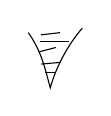
\begin{tikzpicture}[x=.7cm,y=.7cm,baseline=0pt]
\draw (-.4,1) .. controls (-.15,.66) and (-.08,.28) .. (0,0)
 .. controls (.1,.36) and (.31,.77) .. (.58,1.08);
\draw (-.1,.28)--(.1,.28);
\draw (-.16,.43)--(.18,.46);
\draw (-.21,.65)--(.1,.73);
\draw (-.19,.84)--(.34,.84);
\draw (-.17,.96)--(.18,1);
\end{tikzpicture}
\end{adjustbox}]

(3) \underline{Теор.} Ширина $N$-й зоны $\asymp\varepsilon^{[\frac Np]}$,
если $a$ — триг. многочлен, $\operatorname{deg} a=p$.
\Unclear{GELFAND-P001081}{zone-width-exponent}{квадратные скобки $[N/p]$ в показателе степени}

\Unclear{GELFAND-P001081}{mathieu-name}{Матье / Мате}: $p=1$

Ур-е Хилла ($a$ общего положения) $\Rightarrow$
\begin{adjustbox}{max width=\linewidth}
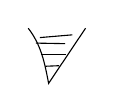
\begin{tikzpicture}[x=.7cm,y=.7cm,baseline=0pt]
\draw (-.37,1) .. controls (-.13,.69) and (-.07,.36) .. (0,0)--(.67,1);
\draw (-.06,.31)--(.19,.32);
\draw (-.14,.52)--(.32,.52);
\draw (-.23,.73)--(.3,.72);
\draw (-.16,.83)--(.43,.88);
\end{tikzpicture}
\end{adjustbox}
всюду касание $1$-го пор.

(но ширина $\exp$ убывает)

\underline{Вопр. ИМГ.:} \underline{$\omega^2$ — $0$-зонный потенциал}.
Что будет вблизи $1$-зонного потенциала?

\underline{Док-во} зав. от структуры ряда Рэлея-Шредингера.
Ищем возмущ.
\begin{equation*}
(4)\quad
(\Lambda+\varepsilon A)(\xi_0+\varepsilon\xi_1+\ldots)
=(\xi_0+\varepsilon\xi_1+\ldots)(\lambda_0+\varepsilon\lambda_1+\ldots)
\end{equation*}

\SourcePage{GELFAND-P001082}{unlabelled}
ряды \Unclear{GELFAND-P001082}{first-line-abbreviation}{сверт. / сверн.}
и зав. от чисел \underline{Каталана}:
\begin{equation*}
1\quad 1\quad 2\quad 5\quad 14\quad 42\quad 138
\end{equation*}
\Unclear{GELFAND-P001082}{catalan-number}{последнее выписанное число: $138$}

Другое появл.: у Гриффитса и Харриса (они не заметили).

\underline{Ф-ла:}
\begin{equation*}
(5)\qquad a_{n+1}=\sum_{j=1}^{n-1}a_j a_{n-j}
\end{equation*}
\Unclear{GELFAND-P001082}{catalan-recurrence}{индексы и пределы суммы в записи источника}

Через произв. ф-ю считаем
\begin{equation*}
a_n=\frac{(2n)!}{n!(n+1)!}
\end{equation*}
($=$ число симплиц. разбиений $n$-угольника)
\Unclear{GELFAND-P001082}{polygon-index}{в скобках написано $n$-угольника}

[Слева над следующей строкой: «Гриффитс, Харрис:».]
Рим. пов. рода $g$ имеют $3g-3$ модуля.

На $S^2=\mathbb C P^1$ выбир. точки ветвления и т.д.

ГХ: число способов, к-рыми получена одна
[зачёркнуто: \Unclear{GELFAND-P001082}{genus-cancel}{пов.?}]
и та же пов.:
\begin{equation*}
1,1,2,5,\ldots\quad\text{— ч. Каталана (но не сказано — почему)}
\end{equation*}

\underline{Скобочный символ:} выраже., правильно сост. из букв.
и скобок: пример
\begin{equation*}
((a))b\,(cd)e
\end{equation*}
\begin{equation*}
\sum\text{числа символов и открыв. скобок}=n\quad\text{(длина)}
\end{equation*}
\begin{equation*}
\Downarrow
\end{equation*}
колич. $=$ числу Каталана

\begin{adjustbox}{max width=\linewidth}
\begin{tikzpicture}[x=1cm,y=.65cm]
\node at (.45,0) {дл. 1};
\node at (1.8,0) {$a$};
\draw (0,-.35)--(2.35,-.35);
\draw (2.5,.45)--(2.5,-2.1)--(.1,-2.1);
\node at (.45,-.9) {дл. 2};
\node at (1.8,-.85) {$ab$};
\node at (1.8,-1.55) {$(a)$};
\draw (1.5,-.55)--(1.35,-.55)--(1.35,-1.95)--(1.5,-1.85);
\node at (4.15,0) {дл. 3};
\draw (3.7,-.35)--(4.65,-.35);
\draw (4.65,.4)--(6.35,.4)--(6.35,-3.4)--(4.65,-3.4)--(4.65,.25);
\node at (5.5,0) {$a(b)$};
\node at (5.5,-.65) {$(a)b$};
\node at (5.5,-1.3) {$(ab)$};
\node at (5.5,-2) {$((a))$};
\node at (5.5,-2.7) {$abc$};
\end{tikzpicture}
\end{adjustbox}

Скоб. символ $\rightsquigarrow$ член ряда теории возмущений.
\begin{equation*}
\underset{\text{соб. числа}}{\lambda_i}\quad\rightsquigarrow\quad\text{колчан}
\end{equation*}

\underline{Соб. числа.}\qquad
$\Lambda$ — диаг. оператор,\qquad $\Lambda_i:V_i\longrightarrow V_i$

(6)
\begin{adjustbox}{max width=\linewidth}
\begin{tikzpicture}[x=.8cm,y=.8cm,baseline=0pt]
\draw (0,-2.3)--(0,.2)--(2.5,.2);
\draw (0,-.4)--(.6,-.4)--(.6,.2);
\node at (.3,-.1) {$\Lambda_i$};
\draw (.6,-.4)--(1.1,-.4)--(1.1,-.9)--(.6,-.9)--(.6,-.4);
\draw[dotted] (1.27,-1.08)--(2.5,-2.3);
\end{tikzpicture}
\end{adjustbox}
\qquad
$\underset{\text{матр. элем. возмущ.}}{A_{i,j}:V_i\longrightarrow V_j}$

колчан:
\begin{adjustbox}{max width=\linewidth}
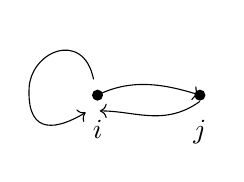
\begin{tikzpicture}[x=1cm,y=1cm,baseline=0pt]
\fill (0,0) circle (2pt);
\fill (1.3,0) circle (2pt);
\node[below] at (0,-.2) {$i$};
\node[below] at (1.3,-.2) {$j$};
\draw[->] (0,0) .. controls (.4,.2) and (.8,.16) .. (1.3,0);
\draw[->] (1.3,-.08) .. controls (.85,-.4) and (.48,-.2) .. (.03,-.2);
\draw[->] (-.05,.2) .. controls (-.18,.85) and (-.88,.55) .. (-.87,.05)
 .. controls (-.88,-.52) and (-.5,-.43) .. (-.15,-.22);
\end{tikzpicture}
\end{adjustbox}
\qquad\underline{стрелке $\rightsquigarrow A_{i,j}$}

$V_i\quad V_j$ — соб. подпр-ва (вершины)

\SourcePage{GELFAND-P001083}{9}
Пусть все конечно или лок. конечно

(в $\forall$ вершину ведёт конечное число)

Ур-е \Unclear{GELFAND-P001083}{mathieu-name-top}{Матье / Мате}
— колчан не полный!

(лок. конечный)

(потенц. — $\cos$ и $\sin$ и соб. ф-и тоже!)

\underline{\Unclear{GELFAND-P001083}{mathieu-name-lower}{Матье / Мате}}
(с триг. многочл.) $\Rightarrow$ матр. типа обобщ. Якобиевой.

Ищем возмущение $\lambda_0$.

\begin{adjustbox}{max width=\linewidth}
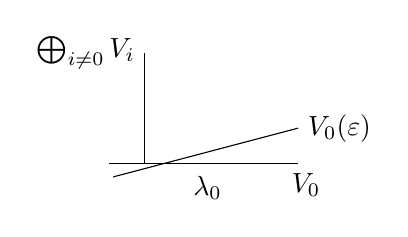
\begin{tikzpicture}[x=1cm,y=1cm]
\draw (-.45,0)--(1.95,0);
\draw (0,0)--(0,1.4);
\draw (-.4,-.17)--(1.95,.45);
\node[left] at (0,1.4) {$\bigoplus_{i\ne0}V_i$};
\node[below] at (2.05,0) {$V_0$};
\node[below] at (.8,-.04) {$\lambda_0$};
\node[right] at (1.95,.45) {$V_0(\varepsilon)$};
\end{tikzpicture}
\end{adjustbox}

$V_0(\varepsilon)$ — подпр-во [подписано ниже: «собств.»],
аналит. завис. от $\varepsilon$, соотв. соб.
\Unclear{GELFAND-P001083}{eigenvalue-word}{вект. / велич.},
близким к $\lambda_0$

\begin{equation*}
(7)\quad (\Lambda+\varepsilon A)(E_0+B(\varepsilon))
=(E_0+B(\varepsilon))(\lambda_0+\varepsilon\alpha^1+\ldots)
\end{equation*}
\Unclear{GELFAND-P001083}{coefficient-symbol}{буква коэффициентов: $\alpha$, возможно $\mathcal L$}

$V_0(\varepsilon)$ — график оператора
\begin{equation*}
B(\varepsilon):V_0\longrightarrow\bigoplus_{i\ne0}V_i
\qquad E_0\text{ — проектор на }V_0
\end{equation*}
\begin{equation*}
\alpha^1:\text{ оператор }V_0\to V_0,\qquad \alpha^i:V_0\to V_0
\end{equation*}

(7) — условие инвариантности
[зачёркнуто: \Unclear{GELFAND-P001083}{invariance-cancel}{неразборчивый знак}]
$V_0(\varepsilon)$

(8) опер. $\lambda_0+\varepsilon\alpha^1+\ldots$ наз.
\underline{\Unclear{GELFAND-P001083}{secular-ending}{секулярный / секулярным; окончание исправлено над строкой}}
опр. (в физике)

Сужение $\Lambda+\varepsilon A$ на $V_0(\varepsilon)$ подобно
секул. опер. (8) $\Rightarrow$ у них одинак. соб. числа.

\underline{Ф-ла для $\alpha^k$:}
\begin{equation*}
(9)\qquad \alpha_k=\sum_{\gamma:\lvert\gamma\rvert=k}
\bigl(\Pi_\gamma(A)Q_\gamma(\Lambda)\bigr)
\end{equation*}
$\gamma$ — петля в колчане из $0$ в $0$

$k$ — длина петли

(10)
\SourceFigure{GELFAND-P001083}{loop-diagram}{Слева внизу $m$,
сверху слева $0$, сверху справа $i$, внизу две подписи, похожие на $j$.
Внутри справа $\gamma$. Видны направленные отрезки от $m$ к $0$,
от $0$ к $i$, от $i$ вниз к правой подписи $j$, диагональ от правой
нижней позиции к $0$, отрезок от $0$ к левой нижней позиции $j$
и от неё влево к $m$. Между двумя нижними подписями проведена
двусторонняя стрелка; у левой позиции имеется дополнительный
короткий наклонный штрих со стрелочным утолщением. Его принадлежность
и точное соединение нижних линий требуют проверки.}
\begin{equation*}
\Pi_\gamma(A)=A_{m0}\ldots A_{ij}A_{0i}
\end{equation*}

$\Pi_\gamma(A)$ — хронологическое произведение петли
($=\prod A_{i,j}$ в нужном порядке по петле)
[Под последними словами приписано: «по стрелкам».]

$Q_\gamma(\Lambda)$ — рац. ф-я от соб. чисел

(вычис. через числа Каталана!)

Рассм. скоб. символ

\underline{Заполнение его} — вставл. вершин колчана вместо букв.
\SourcePage{GELFAND-P001084}{unlabelled}
% Additional inspected crop review1084-heading-ending: [1280, 1390, 2010, 1535], 6x.
% Original image: 2408 x 3448 pixels. Coordinates below refer to the original,
% with origin at the upper-left; enlargements do not add source detail.
По заполнению строится петля.

[Зачёркнуто: \Unclear{GELFAND-P001084}{top-cancel}{неразборчивый знак}.]
Слагаемые надо нумеровать заполнениями

\begin{center}
\begin{adjustbox}{max width=\linewidth}
\begin{tikzcd}
\Vert\quad 0 \arrow[r] & 0 \arrow[r] & i \arrow[r] & j \arrow[r] & 0
\end{tikzcd}
\end{adjustbox}
\end{center}

\begin{equation*}
\begin{array}{cl}
(i)j & \\
\downarrow & \\
0 & \text{по открытой скобке,}
\end{array}
\end{equation*}
\Unclear{GELFAND-P001084}{bracket-rule}{закрытые опускаем / закрытую опускаем}

Стрелок на 1 больше, чем длина заполнения.

1 петля — из разных заполнений.

\begin{center}
\begin{adjustbox}{max width=\linewidth}
\begin{tikzcd}
0 \arrow[r] & i \arrow[r] & j \arrow[r] & 0 \arrow[r] & j \arrow[r] & m \arrow[r] & 0
\end{tikzcd}
\end{adjustbox}
\end{center}

Сумма на самом деле не по петлям, а заполнениям

[Зачёркнута строка:
\Unclear{GELFAND-P001084}{cancelled-fillings}{$ij(jm)\quad ij(jm)$; справа «не од…»}.]

\begin{equation*}
ij(jm
\end{equation*}
не однозн. закрыв. скобка!! —

[Обведено: повтор.]
[Зачёркнуто: \Unclear{GELFAND-P001084}{cancelled-before-exit}{— это не / — тот же}.]
выход
[Зачёркнуто: \Unclear{GELFAND-P001084}{cancelled-after-exit}{разные скобки!! / нужные скобки!!}.]

Диаграмма заполнения: добавл. пунктирные
[Окончание слова «пунктирные» переписано:
\Unclear{GELFAND-P001084}{overwritten-adjective-ending}{«ые» поверх прежних штрихов; возможное прежнее «ую» не установлено}.]
[зачёркнуто: скобки; ниже вписано: стрелки]

% Diagram reviewed at 3x: original crop (140,1510,1280,1835).
\begin{center}
\begin{adjustbox}{max width=\linewidth}
\begin{tikzpicture}
\node at (-1.8,0) {$(i)j$};
\node (z1) at (0,0) {$0$};
\node (z2) at (1.3,0) {$0$};
\node (ii) at (2.6,0) {$i$};
\node (jj) at (3.9,0) {$j$};
\node (z3) at (5.2,0) {$0$};
\draw[->] (z1) -- (z2);
\draw[->] (z2) -- (ii);
\draw[->] (ii) -- (jj);
\draw[->] (jj) -- (z3);
\draw[->,dashed] (ii.north) to[bend right=55] (z2.north);
\draw (0,-0.4) -- (0,-0.85) -- (-0.7,-0.85);
\draw (5.0,-0.4) -- (5.0,-0.7) -- (6.0,-0.7);
\end{tikzpicture}
\end{adjustbox}
\end{center}
крайние нули ничего не значат

Стрелка $\longrightarrow$ в $0$, соотв. открыв. скобке, соответствующей
[зачёркнуто: \Unclear{GELFAND-P001084}{cancelled-open}{открыв. / открыт.}]
закрыв. скобке (из буквы до закрыв. скобки)

% Equation and its annotations reviewed at 3x:
% (315,2030,1110,2545); the product note at (390,2570,2170,2705).
\begin{equation}
\mathcal{L}_k=
\sum_{I,\ |I|=k-1}\frac{\Pi_{\gamma(I)}(A)}{q_I(\Lambda)}
\tag{11}
\end{equation}
[Под $I$ проведена короткая вертикальная черта к пояснению:]
заполнение скоб. \Unclear{GELFAND-P001084}{bracket-symbol-ending}{символа / символ}

$|I|$ — длина скоб. \Unclear{GELFAND-P001084}{bracket-symbol-ending}{символа / символ}

$\Pi_{\gamma(I)}(A)$ — хрон. произв. петли по сплошным стрелкам.

\begin{equation}
q_I(\Lambda)=
\underset{\substack{\text{сплошные}\\\text{стрелки}\\\text{в }i}}
{\prod_{i\ne0}}(\lambda_0-\lambda_i)
\underset{\substack{\text{пункт.}\\\text{стрелки}\\\text{из }j}}
{\prod_{j\ne0}}(\lambda_j-\lambda_0)
\tag{12}
\end{equation}

% Last formula reviewed at 3x: (390,3160,1680,3320).
\begin{equation*}
(i)j\rightsquigarrow
(\lambda_0-\lambda_i)(\lambda_0-\lambda_j)(\lambda_i-\lambda_0)
\end{equation*}

\SourcePage{GELFAND-P001085}{10}
% Original image: 2408 x 3448 pixels; upper text reviewed at 3x,
% original crop (270,30,1790,300).
Для четных триг. многочленов достат. ф-ы (9)

[Под словом «четных»: $(\text{по }\cos)$]

(и отдельно для $\sin$ тоже)

\begin{equation*}
V=\bigoplus V_i
\end{equation*}

\begin{equation}
\Lambda=\frac{d^2}{dt^2},\qquad
V_k=\{e_k,e_{-k}\},\qquad e_k=e^{ikt}
\tag{13}
\end{equation}

% Subscripts and dimensional annotations reviewed at 3x:
% original crop (300,460,1700,870).
\begin{equation*}
\begin{array}{c c c c c c c}
 & V_0 & V_1 & V_2 & V_3 & \cdots & V_k\\
\dim & 1 & 2 & 2 & 2 & & 2\\
 & & & & & & \lambda=-k^2
\end{array}
\end{equation*}

$A$ — умн. на триг. многочлен

\begin{equation}
a(t)=\sum_{|s|\le p}a_se_s
\tag{14}
\end{equation}

Пусть он чётный, т.е.

\begin{equation}
a_{-s}=a_s
\tag{15}
\end{equation}

% Matrix reviewed at 4x: original crop (440,1420,1620,1695).
\begin{equation}
A_{i,j}=
\begin{pmatrix}
a_{j-i} & a_{i+j}\\
a_{-i-j} & a_{i-j}
\end{pmatrix}
\qquad (?)
\tag{16}
\end{equation}

$(16)\Rightarrow$ если $i+j>p$, то матрицы диагон. и даже
\underline{скалярны} [ниже: (ввиду (15))] в этом базисе.

Если все $A_{i,j}$ в петле скалярны, то и произвед. скалярно.

\begin{equation}
\underline{\tau p<2k}\quad\Rightarrow\quad
\mathcal{L}_\tau\ \text{скалярно}
\tag{17}
\end{equation}
[«$\mathcal{L}_\tau$ скалярно» подчёркнуто волнистой линией.]

Это — топологич. лемма (из комбинат. топ.)

\underline{Д-во}

% The fourteen visible ticks and their positions are retained.
% Number line reviewed at 3x: original crop (300,2320,1800,2990).
\begin{center}
\begin{adjustbox}{max width=\linewidth}
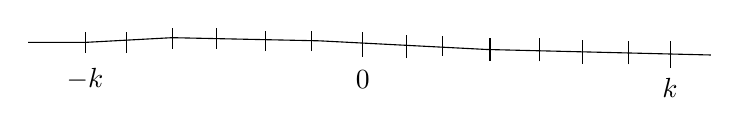
\begin{tikzpicture}[x=0.85cm,y=1cm]
\draw (-0.85,0) -- (0,0) -- (1.3,0.06) -- (3.5,0.02) -- (6,-0.09) -- (9.35,-0.16);
\draw (0,-0.13) -- (0,0.13);
\draw (0.62,-0.13) -- (0.62,0.13);
\draw (1.31,-0.08) -- (1.31,0.18);
\draw (1.96,-0.08) -- (1.96,0.18);
\draw (2.70,-0.11) -- (2.70,0.15);
\draw (3.38,-0.11) -- (3.38,0.15);
\draw (4.15,-0.18) -- (4.15,0.13);
\draw (4.80,-0.20) -- (4.80,0.10);
\draw (5.34,-0.17) -- (5.34,0.08);
\draw (6.05,-0.23) -- (6.05,0.05);
\draw (6.79,-0.24) -- (6.79,0.05);
\draw (7.43,-0.27) -- (7.43,0.03);
\draw (8.12,-0.28) -- (8.12,0.02);
\draw (8.74,-0.32) -- (8.74,0.02);
\node at (0,-0.47) {$-k$};
\node at (4.15,-0.47) {$0$};
\node at (8.74,-0.58) {$k$};
\end{tikzpicture}
\end{adjustbox}
\end{center}

Рассм. петлю из $\tau$ стрелок длины $\le p$.

Тогда для $\forall$ стрелки $i+j>p$

(гомотопна $0$!)

$i+j\le p\ \Rightarrow$
\Unclear{GELFAND-P001085}{crossing-word}{перескок / перемена}

\SourceFigure{GELFAND-P001085}{loop-arches}{Три соседние дуги: большая слева, малая посередине и большая справа; под левым концом стоит $-k$, под правым $+k$. В двух внутренних стыках видны острые нисходящие штрихи; их чтение как наконечников стрелок требует проверки. У правого конца имеется отдельный знак, похожий на $i$; его чтение и отношение к дугам не установлены.}
$\Rightarrow$ длина $\le\tau p$ и т.д.

$(17)\Rightarrow$ в этом приближении соб. число ещё не расщепилось
$\Rightarrow$

$\Rightarrow$ нужное нер-во!

\SourcePage{GELFAND-P001086}{unlabelled}
% Additional inspected crop root-review1086-final-abbreviation: [1180, 1130, 1450, 1250], 7x.
% Original inspected directly at 2408 x 3448. Text crops: [160,40,1270,425], [130,430,2110,800], [165,800,1720,1300], each 3x.
% Bracket-word crops: [225,170,760,300], [270,425,970,570], [270,675,945,810], [250,925,800,1060], each 6x.
% Additional word crops [175,550,425,690] and [610,295,910,420], each 6x. The rest of the frame below the final line is blank.
Ещё используется инволюция:
\begin{equation*}
(((a))b)(cd)e
\end{equation*}
откр. скобками разбив. на фрагменты
\begin{equation*}
a))b)\qquad cd)e
\end{equation*}
Закрыв. скобки приклеиваем к букве. Переставл. буквы во фрагментах
[приписано ниже слева: в обр. порядке]
\begin{equation*}
b)a))\qquad ed)c
\end{equation*}
[зачёркнуто: \Unclear{GELFAND-P001086}{cancel-before-stavim}{ост. / вст.}]
Ставим откр. скобки на старые места
\begin{equation*}
(((b)a))(ed)c
\end{equation*}
\underline{Получ. двойств. символ}

Его вклад получается перестан. \Unclear{GELFAND-P001086}{final-abbreviation}{диаг. / диам.} элементов.

\SourcePage{GELFAND-P001087}{unlabelled}
% Original inspected directly at 2408 x 3448; top area preceding the dated heading is blank.
% Text crops at 3x: [160,875,1100,1130], [255,1120,2110,1230], [160,1230,1510,1480], [150,1480,2020,2010], [315,2010,2030,2430], [145,2420,1520,3040], [440,3035,960,3270].
% Rechecks: [1480,1115,1850,1230] 6x; [1795,1115,2120,1230] 8x; [520,1390,725,1480] 10x; [900,1810,1060,2000] 8x; [1410,1695,1980,1810] 6x; [1350,2130,1545,2250] 8x; [670,2210,1160,2420] 6x; [460,3140,950,3250] 6x.
\underline{28/II-83 г.}\qquad \underline{\underline{Сем. Гельфанда.}}

\underline{И. Кричевер.}

Цель --- построить формальную теорию возмущ. для возмущения ур-я КдФ.
\begin{equation*}
\text{(1)}\qquad
u_t-\frac{\partial}{\partial x}
\underbrace{\left(\frac{1}{4}u_{xx}-\frac{3}{4}u^2\right)}_{\frac{\delta I_3}{\delta u}}
=\varepsilon K[u]
\end{equation*}
[Под $K$: дифф. полином от $u$.]

[Зачёркнуто: $u=u_0$.]
\begin{equation*}
\text{(2)}\qquad u=u_0(x,t)+\varepsilon(\ldots)
\end{equation*}
КдФ
\begin{equation*}
\text{(3)}\qquad
u_t-\frac{\partial}{\partial x}
\underbrace{\left(\frac{1}{4}u_{xx}-\frac{3}{4}u^2\right)}_{\frac{\delta I_3}{\delta u}}
=0,\qquad I_3=\frac{1}{4}(u_x^2+u^3).
\end{equation*}
[Нижние скобы под скобочными выражениями в (1) и (3) в рукописи прямоугольные.]
[Между нижней скобкой и её подписью: \Unclear{GELFAND-P001087}{eq03-variational-annotation}{$\Vert$}.]

Имеется беск. серия инволют. интегралов $I_k$: $I_1=u$, $I_2=u^2$, $\ldots$

Конечнозонное реш. --- реш. --- стац. точка ф-ла
\begin{equation*}
\text{(4)}\qquad H=I_{n+2}-\sum_{k=1}^{n+1}c_k I_k
\end{equation*}
т. е. решение ур-я
\begin{equation*}
\text{(5)}\qquad \frac{\delta H}{\delta u}=0
\end{equation*}
Рекурр. соотношение:
\begin{equation*}
\text{(6)}\qquad
\frac{d}{dx}\frac{\delta I_{n+1}}{\delta u}
=\left[\left(\frac{d}{dx}\right)^3+2u\frac{d}{dx}+u'\right]
\frac{\delta I_n}{\delta u}
\end{equation*}
(с точн. до коэффициентов).
\begin{equation*}
\delta^2 H\; -\; ?
\end{equation*}
в опр. стац. точке.

\SourcePage{GELFAND-P001088}{15}
% Original inspected directly at 2408 x 3448. Content reviewed continuously from the operator and spectrum to the bottom task.
% Broad crops at 3x: [305,40,2030,455], [150,455,1670,940], [365,935,2260,1360], [275,1360,1770,2005], [320,2000,2260,2550], [130,2550,2230,3030], [300,3010,2220,3435].
% Local rechecks: [1130,60,1460,180] 8x; [1120,530,1360,670] 8x; [1620,710,1880,850] 10x; [1730,1990,2320,2130] 5x; [750,2290,1060,2490] 8x; [1530,2350,2340,2600] 4x; [610,2680,1070,2830] 6x; [690,2820,1170,2970] 6x; [770,2940,1250,3060] 8x; [1135,3140,1620,3290] 8x; [295,3270,1030,3425] 5x.
\begin{equation*}
L=-\frac{d^2}{dx^2}+u_0(x)\qquad
\text{спектр:}\qquad (u_0(x+1)=u_0(x))
\end{equation*}
% Upper spectrum: four finite segments, then a segment extending right without an arrowhead; endpoint labels only where written.
\begin{center}
\begin{adjustbox}{max width=\linewidth}
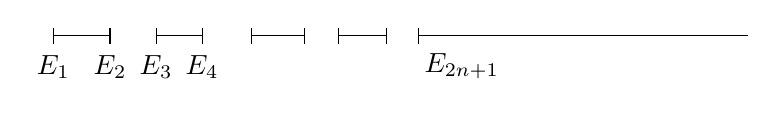
\begin{tikzpicture}[x=0.9cm,y=0.65cm]
\draw (0,0)--(0.8,0);
\draw (0,-0.15)--(0,0.15);
\draw (0.8,-0.15)--(0.8,0.15);
\draw (1.45,0)--(2.1,0);
\draw (1.45,-0.15)--(1.45,0.15);
\draw (2.1,-0.15)--(2.1,0.15);
\draw (2.8,0)--(3.55,0);
\draw (2.8,-0.15)--(2.8,0.15);
\draw (3.55,-0.15)--(3.55,0.15);
\draw (4.02,0)--(4.7,0);
\draw (4.02,-0.15)--(4.02,0.15);
\draw (4.7,-0.15)--(4.7,0.15);
\draw (5.15,0)--(9.8,0);
\draw (5.15,-0.15)--(5.15,0.15);
\node[below] at (0,-0.2) {$E_1$};
\node[below] at (0.8,-0.2) {$E_2$};
\node[below] at (1.45,-0.2) {$E_3$};
\node[below] at (2.1,-0.2) {$E_4$};
\node[below right] at (5.1,-0.15) {$E_{2n+1}$};
\end{tikzpicture}
\end{adjustbox}
\end{center}
Оставшиеся концы --- простые соб. знач. периодич. и антипер. задач.

Дифференциал квазиимпульса:
\begin{equation*}
\text{(7)}\qquad
 i\,dp=\frac{Q(E)dE}{\sqrt{R}}
 =\frac{E^n+\sum_{k=1}^{n}r_k E^{n-k}}{\sqrt{R}}\,dE
\end{equation*}
[Коэффициент в числителе: \Unclear{GELFAND-P001088}{eq07-polynomial-coefficient}{$r_k$ / $\gamma_k$ / $\tau_k$}.]
\begin{equation*}
R(E)=\prod_{i=1}^{2n+1}(E-E_i)
\end{equation*}
[Зачёркнуто справа: \Unclear{GELFAND-P001088}{cancel-normalized}{(норм. / (нормир.}]

Условия, однозначно определяющие $dp$:
\begin{equation*}
\int_{E_{2i}}^{E_{2i+1}}dp=0
\end{equation*}
(нормир. абелев дифференциал\newline
2-го рода с единств. особ. на $\infty$ ---\newline
--- полюс 2-го пор.)

Рассм. теперь возмущение $u=u_0+\delta u$

$E_i'$ --- новые концы зон

$e_s^-<e_s^+$ --- новые концы зон; $\delta e_s=e_s^+-e_s^-$

Тогда:
\begin{equation*}
\text{(8)}\qquad
\delta^2H=\frac{1}{2}\sum Q(E_i)(\delta E_i)^2
+\frac{1}{4}\sum_s Q(e_s)(\delta e_s)^2
\end{equation*}
($e_s$ --- 2-кратные точки спектра)

$Q$ меняет знак по 1 разу в $\forall$ из запрещ. зон $\Rightarrow$ по 1-му нулю
в любой зоне

% Lower sign diagram: the upward annotation arrow points inside the finite segment bearing the minus sign.
\begin{center}
\begin{adjustbox}{max width=\linewidth}
\begin{tikzpicture}[x=0.85cm,y=0.7cm]
\node at (-0.9,0) {$\ldots$};
\draw (0.6,0)--(1.2,0);
\draw (0.6,-0.13)--(0.6,0.13);
\draw (1.2,-0.13)--(1.2,0.13);
\node at (0.95,0.55) {$+$};
\draw (2.35,0)--(3.15,0);
\draw (2.35,-0.13)--(2.35,0.13);
\draw (3.15,-0.13)--(3.15,0.13);
\node at (2.8,0.55) {$-$};
\draw[->] (4.35,0)--(8.15,0);
\draw (4.35,-0.13)--(4.35,0.13);
\node at (5.8,0.55) {$+$};
\node at (10.65,0.4) {знак $Q$};
\draw (9.55,-0.12) .. controls (9.72,0.04) and (9.89,-0.22) .. (10.06,-0.10)
.. controls (10.23,0.04) and (10.40,-0.21) .. (10.57,-0.10)
.. controls (10.74,0.04) and (10.91,-0.21) .. (11.08,-0.10)
.. controls (11.25,0.04) and (11.42,-0.21) .. (11.60,-0.08);
\draw[->] (2.48,-1.1)--(2.7,-0.3);
\end{tikzpicture}
\end{adjustbox}
\end{center}
[Под стрелкой:] внутри [зачёркнуто: \Unclear{GELFAND-P001088}{cancel-before-mogut}{будут / буд.}]
могут быть ещё слипшиеся $\Rightarrow$ доб. ещё
полож. или отриц. квадрат\newline
(из 2-й суммы в (8))

\begin{equation*}
\text{(9)}\qquad L\Psi(x,E)=E\Psi
\end{equation*}
\begin{equation*}
\Psi(x+1)=w\Psi,\qquad w=e^{iP},\qquad P=\int_{E_1}^{E}dp
\end{equation*}
Ширина раскр. зоны
\begin{equation*}
\text{(10)}\qquad
(\delta e_s)^2=
\frac{|\langle(\delta u)\Psi^2\rangle|^2}{\langle|\Psi|^2\rangle}
\end{equation*}
[Знаменатель (10): \Unclear{GELFAND-P001088}{eq10-denominator}{$\langle|\Psi|^2\rangle$}.]
($\Psi$ --- блох. ф-я, $\Psi(x,e_s)$)

$\langle\qquad\rangle$ --- усредн. по периоду

$u_0=\mathrm{const}\Rightarrow$ получ. [зачёркнуто: средн… \Incomplete{GELFAND-P001088}{cancel-before-fourier}{Дальнейшее слово или короткая группа слов закрыты плотными линиями зачёркивания; прочесть их не удалось.}] коэфф. Фурье для
возмущения.

\underline{Задача (ИМГ)}: посчитать 3-ю вариацию и т. п.

\SourcePage{GELFAND-P001089}{unlabelled}
% Additional inspected crop root-review1089-coefficient: [1100, 190, 1550, 325], 7x.
% Additional inspected crop root-review1089-psi: [245, 770, 675, 920], 5x.
% Additional inspected crop root-review1089-speaker: [135, 2705, 315, 2865], 7x.
% Additional inspected crop peer-review1089-positive-coefficient: [775, 190, 1100, 325], 8x.
% Eq.(11) coefficient review: [775,190,1100,325] at8x and [1100,190,1550,325] at7x. Right a bounding box [1281,267,1315,301], s [1306,287,1325,314], superscript minus [1326,250,1348,256]; retained a_s^-. Psi rechecked [245,770,675,920] at5x.
% Additional resolved crop checks: KdF [1010,355,1230,475] at 8x; zone wording [570,465,1250,585] at 5x; speaker heading [295,1460,850,1595] at 5x and [565,1480,835,1580] at 10x; adjoint wording [1060,810,1370,930] at 6x; lower note [1110,2820,2100,2935] at 5x and [1160,2700,2100,2920] at 5x.
% Direct original and 3x page-region reviews: [120,45,2300,760], [110,785,2080,1460], [70,1450,1730,2220], [65,2260,2260,3270].
Вернемся к (1); пусть $u$ — решение. Тогда в 1-м пор. по $\varepsilon$
\begin{equation*}
u(x,t)=u_0(x,t)+\varepsilon\sum_s
\bigl[a_s^+w_s^+(x,t)+a_s^-w_s^-(x,t)\bigr]\tag{11}
\end{equation*}
$w_s^\pm(x,t)$ — реш. линеариз. КдФ в окр. $n$-зонного решения.
Они наход. так: проращиваем зону в окр. $e_s$ и берем производную по длине нов. зоны.
[Над словами «берем производную» вставлено: «$(n+1)$-зон. потенц.»]
\begin{equation*}
w_s^\pm(x,t)=-2\frac{\partial^2}{\partial x^2}
\ln\theta\bigl(Ux+Vt+Z-A(e_s)\bigr)e^{2\pi isx+V_st}\tag{12}
\end{equation*}
[В аргументе $\theta$ над строкой вставлено: $Vt+$ перед $Z$.]
\Unclear{GELFAND-P001089}{upper-formula-frequency}{В показателе экспоненты: $V_st$ или $\Gamma_st$.}

$\Psi^2_{s\pm}(x,t,E)$ — реш. ур-я, сопряж. к линеариз. ур-ю $KdV$.
\begin{equation*}
\left\langle\Psi^2_{s\pm}(x,t,E),w_s^\pm(x,t)\right\rangle=0,
\qquad s\ne s'\tag{13}
\end{equation*}
(средн. по $x$)
\Unclear{GELFAND-P001089}{middle-orthogonality-indices}{В обоих множителях читается индекс $s$; справа написано $s\ne s'$.}

($\Rightarrow$ имеется разл. по базису)
\begin{equation*}
w_s^\pm,\quad \frac{\partial u}{\partial E_i},\quad
\frac{\partial u}{\partial\gamma_i}
\end{equation*}
\Unclear{GELFAND-P001089}{middle-parameter-derivative}{Знаменатель последней производной: $\partial\gamma_i$ или $\partial\delta_i$.}

\bigskip
\underline{\underline{Водзицки (Мариус).}}
\begin{equation*}
L_w=-\frac{d^2}{dx^2}+u(x)-w,\qquad x\in[0,T]\tag{1}
\end{equation*}
(\underline{опер. Хилла}; $u$ — $T$-периодич.)

$\zeta$-ф-я:
\begin{equation*}
\zeta_{L_w}(s)=\sum_{\substack{\lambda\in\operatorname{Spec}L\\\lambda\ne w}}
(\lambda-w)^{-s},\qquad \operatorname{Re}s>\tfrac12.\tag{2}
\end{equation*}
Интересуемся: значениями в т. $s=1,2,3,\ldots$

Пусть
\begin{equation*}
\begin{gathered}
u(x)\text{ — конечнозонный},\\
w\in\{\alpha_0,\ldots,\alpha_{2n}\}\text{ — концы зон}
\end{gathered}\tag{3}
\end{equation*}

\underline{И.М.Г.} \underline{Костя:}

\Unclear{GELFAND-P001089}{lower-speaker-abbreviation}{Доп: / Дан:}
\underline{Hurwitz} 1899
\Unclear{GELFAND-P001089}{lower-hurwitz-overwritten-word}{[густо переписанное короткое слово: неразборчиво]}
$\displaystyle\sum\frac{1}{(n+a)^s}$

$\displaystyle\sum_n\frac{1}{(n^2+a)^s}$ — прод. с беск. числом полюсов

[От суммы проведена выноска к надписи:] $\zeta$-ф-я Эпштейна.

однор. полином: \underline{есть функц. ур-е.}
\begin{equation*}
\frac{1}{(n^2+a)^s}
=\frac{1}{\bigl(n^2(1+\frac{a}{n^2})\bigr)^s}
=\left(\frac{1}{n^2}-\frac{a}{n^4}+\frac{a^2}{n^6}+\cdots\right)^s
=\frac{1}{n^{2s}}\left(-\frac{as}{n^{2s+2}}+\cdots\right)
\end{equation*}
\Unclear{GELFAND-P001089}{lower-series-final-equality}{Последнее выражение переписано с видимыми $n^{2s}$ и $n^{2s+2}$; в скобке перед минусом отдельной единицы не видно.}

\underline{Вопрос ИМГ.:} какая арифметика, когда $a$ — рац. число.

\SourcePage{GELFAND-P001090}{16}
% Additional crop checks: differential abbreviation [415,440,1330,580] at 5x; last argument in (6) [1230,1510,1515,1625] at 10x; denominator of (7) [1730,1910,2320,2050] at 10x; summation conditions [1365,1945,1710,2190] at 8x; last monomial [1750,2145,2150,2240] at 10x.
% Direct original and 3x region reviews: [55,20,2300,575], [380,530,2170,1100], [95,1100,2130,1750], [90,1760,2350,2260], [95,2240,1980,3190].
\underline{М.В.}
\begin{equation*}
T\frac{\displaystyle\prod_{i=1}^{n}(z-\alpha_i')}
{\sqrt{4(z-\alpha_0)\cdots(z-\alpha_{2n})}}\,dz
\equiv T\varphi_\alpha(z)\frac{dz}{2\sqrt{z-\alpha}},
\qquad\alpha\in\{\alpha_0,\ldots,\alpha_{2n}\}\tag{4}
\end{equation*}
(опр. $\varphi_\alpha$)

(то же, что выше у Кричевера)
— дифф. квазиимп.

\SourceFigure{GELFAND-P001090}{upper-monodromy-graph}{График с горизонтальной осью и стрелкой вправо; подпись у стрелки похожа на $v$ или $\nu$. В начале оси отмечено $\alpha_0$; от этой точки вверх проведена штриховая вертикаль к пересечению кривой с верхней направляющей. Кривая спускается с верхнего левого края, проходит через первый минимум ниже нижней горизонтальной направляющей, затем через максимум выше верхней направляющей, второй минимум ниже нижней направляющей, следующий максимум на верхней направляющей и следующий минимум чуть выше нижней направляющей. У первого провала стоят $\alpha_1$, $\alpha_1'$, $\alpha_2$; от двух пересечений нижней направляющей и от минимума проведены штриховые вертикали к оси. У следующего максимума подпись $\alpha_2'$, у следующего минимума $\alpha_3'$; от экстремумов идут штриховые вертикали. Верхняя и нижняя направляющие местами прерывисты; между пересечениями с кривой видны утолщенные горизонтальные отрезки на обеих направляющих. Справа от графика: «След матрицы монодромии. $\operatorname{tr}\widehat T(w)$».}

\underline{$\alpha_j'$ — точки $\min$ и $\max$}
$\operatorname{tr}\widehat T(w)$.

Введ. Универ. набор полиномов:
\begin{equation*}
F(u)=1+\sum_{i=1}^{\infty}c_i\frac{u^i}{i!}\tag{5}
\end{equation*}
и тогда
\begin{equation*}
\left[u\frac{d}{du}+p\right][F(u)]^p
=p\cdot\sum_{k=0}^{\infty}Q_{p,k}(c_1,\ldots,c_k)\frac{u^k}{k!},
\qquad Q_{p,0}\equiv1.\tag{6}
\end{equation*}
(определение $Q_{p,k}$)

\begin{equation*}
\begin{aligned}
\widehat Q_{p,k}
&\equiv\frac{p+2k}{p+k}Q_{p,k}(c_1,\ldots,c_k)\\
&=\frac{p+2k}{p}\,k!
\sum_{\substack{|\beta|\le\min(k,p)\\\sum_{i=1}^k i\beta_i=k}}
\binom{p}{|\beta|}
\frac{|\beta|!}{(1!)^{\beta_1}\beta_1!\cdots(k!)^{\Lambda_k}\beta_k!}
\times c_1^{\beta_1}\cdots c_k^{\beta_k}
\end{aligned}\tag{7}
\end{equation*}
\Unclear{GELFAND-P001090}{middle-factorial-exponent}{Показатель при $(k!)$ похож на $\Lambda_k$ или $\lambda_k$; возможное $\beta_k$.}
\begin{equation*}
\sum[F(u)]^p z^p=\frac{1}{1-zF(u)}=\Phi(u,z)
\end{equation*}
и надо взять:
\begin{equation*}
\left(u\frac{\partial}{\partial u}+z\frac{\partial}{\partial z}\right)\Phi(u,z).
\end{equation*}
\begin{equation*}
\log F(u)\equiv\sum Q_{0,k}(c_1,\ldots,c_k)\frac{u^k}{k}\tag{8}
\end{equation*}
\Unclear{GELFAND-P001090}{lower-logarithm-denominator}{Знаменатель под $u^k$ густо переписан: $k$; возможное $k!$ неразличимо.}
(опред. $Q_{0,k}$)

Построим:
\begin{equation*}
\xi_{-1}:=\varphi_\alpha^2(w)\big|_{w=\alpha},\tag{9}
\end{equation*}
\begin{equation*}
\xi_i:=\frac{1}{2i+1}
\left.\frac{\varphi_\alpha^{(i)}(w)}{\varphi_\alpha(w)}\right|_{w=\alpha},
\qquad i=1,2,\ldots\tag{10}
\end{equation*}

\SourcePage{GELFAND-P001091}{unlabelled}
% Additional inspected crop root-review1091-hochstadt: [995, 1580, 1200, 1690], 7x.
% Additional resolved crop checks: eta identity [395,2875,870,3030] at 6x; elliptic symbol [370,2430,710,2550] at 8x.
% Direct original and 3x region reviews: [60,40,2350,730], [295,735,1640,1690], [95,1630,2180,2860], [230,2860,2000,3320].
\begin{equation*}
\begin{aligned}
\zeta(m;L_\alpha)
&=-2Q_{0,m}(\xi_1,\ldots,\xi_m)
+\sum_{p=1}^m\frac{2^{2p}|B_{2p}|}{(2p)!(m-p)!}
\widehat Q_{2p,m-p}(\xi_1,\ldots,\xi_{m-p})\xi_{-1}^p\\
&=-2Q_{0,m}(\xi_1,\ldots,\xi_m)
+\sum_{p=1}^m\frac{\zeta_0(p)}{(m-p)!}
\widehat Q_{2p,m-p}(\xi_1,\ldots,\xi_{m-p})\xi_{-1}^p
\end{aligned}\tag{11}
\end{equation*}
[Под первой строкой:] $\alpha\in\operatorname{Spec}L$.

$\zeta_0$ — $\zeta$-ф-я $-\dfrac{d^2}{dx^2}$ на $[0,T]$.
\begin{equation*}
\zeta_0(s)=\operatorname{Tr}\left(-\frac{d^2}{dx^2},[0,T]\right)^{-s}
\end{equation*}
Через $\zeta$ — $\zeta$-ф-ю Римана
\begin{equation*}
T=2\pi,\qquad\zeta_0(s)=2\zeta_{\mathrm{Riemann}}(2s).
\end{equation*}
\Unclear{GELFAND-P001091}{upper-bernoulli-coefficient}{В первой строке (11) коэффициент $2^{2p}|B_{2p}|/(2p)!$; во второй — $\zeta_0(p)$, при последующем $T=2\pi$.}

0-зонный $\Rightarrow$ выживает 1 чл.

% Separator reviewed on original [875,1460,1100,1485].
\begin{center}
— · —
\end{center}

$u(x)\equiv u_0=\mathrm{const}$
$\Rightarrow$ ф-ла становится банальной

(\Unclear{GELFAND-P001091}{middle-hochstadt-word}{форма / ферма} Хохштадта)
\begin{equation*}
\frac{T\,dz}{\sqrt{4(z-u_0)}}
\end{equation*}
\begin{equation*}
\zeta(m;L_{u_0})=\frac{2^{2m}|B_{2m}|}{(2m)!}
\end{equation*}

\underline{1-зонный}
\begin{equation*}
\omega\frac{z-\eta/\omega}{\sqrt{4z^3-g_2z+g_3}}
\end{equation*}
(\Unclear{GELFAND-P001091}{lower-cubic-prefix}{ф.: / $\wp$:}
$4x^3-g_2x-g_3$)
[Справа выноска к выражению: «ур-е кривой».]

в канонич. обозначениях
\Unclear{GELFAND-P001091}{lower-cubic-signs}{В двух подкоренных выражениях видно $+g_3$; в записи при выноске — $-g_3$.}

\underline{$u=2\wp(x)$}
[Подчеркивание с загнутыми вверх концами.]
% Bracket under u=2wp(x): original [310,2410,820,2610], reviewed at 6x.

% Left period axes: direct original crop [105,2530,735,2770], reviewed at 5x.
\begin{adjustbox}{max width=\linewidth}
\begin{tikzpicture}[x=1cm,y=1cm]
\draw[->] (0,0) -- (0.1,1.2);
\draw[->] (0,0) -- (1.8,0.1);
\node[anchor=east] at (0.02,1.15) {$\omega_1=\omega'$};
\node[anchor=west] at (1.85,0.1) {$\omega=\omega_2=T$};
\end{tikzpicture}
\end{adjustbox}\hspace{1cm}%
% Right graph: original bounds [925,2440,1460,2810], reviewed in the 3x elliptic region and [980,2445,1160,2770] at 8x.
\begin{adjustbox}{max width=\linewidth}
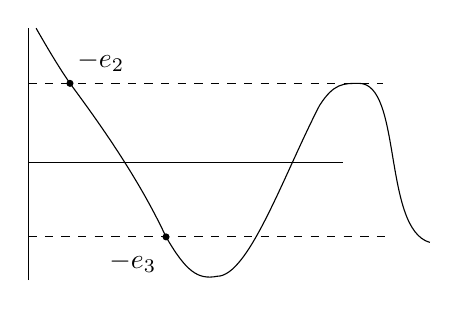
\begin{tikzpicture}[x=1cm,y=1cm]
\draw (0,-1.5) -- (0,1.7);
\draw (0,0) -- (4.0,0);
\draw[dashed] (0,1.0) -- (4.5,1.0);
\draw[dashed] (0,-0.95) -- (4.6,-0.95);
\draw (0.1,1.7) .. controls (0.3,1.35) and (0.42,1.16) .. (0.53,1.0)
.. controls (0.9,0.5) and (1.4,-0.2) .. (1.75,-0.95)
.. controls (2.0,-1.38) and (2.15,-1.5) .. (2.4,-1.45)
.. controls (2.8,-1.45) and (3.25,-0.15) .. (3.7,0.72)
.. controls (3.88,1.0) and (4.0,1.0) .. (4.2,1.0)
.. controls (4.75,1.0) and (4.5,-0.85) .. (5.1,-1.02);
\fill (0.53,1.0) circle (0.045);
\fill (1.75,-0.95) circle (0.045);
\node[anchor=south west] at (0.5,1.02) {$-e_2$};
\node[anchor=north east] at (1.75,-1.02) {$-e_3$};
\end{tikzpicture}
\end{adjustbox}

\begin{equation*}
\frac{\eta}{2}=\zeta\left(\frac{\omega}{2}\right)
\end{equation*}
\begin{equation*}
\omega\zeta\bigl(\wp^{-1}(-w)\bigr)-\eta\wp^{-1}(-w)
=i\omega\int_{-e_2}^{w}
\frac{\bigl(z-\eta(\omega)\bigr)}{\sqrt{4z^3-g_2z+g_3}}\,dz
\end{equation*}
\Unclear{GELFAND-P001091}{bottom-integrand-eta}{В числителе: $z-\eta(\omega)$ или $z-\eta/\omega$; после $\omega$ видны две закрывающие скобки.}

% Bottom separator reviewed on original [510,3280,1140,3320].
\begin{center}
— · —
\end{center}

\SourcePage{GELFAND-P001092}{17}
% Additional inspected crop 1092-top-a: [150, 35, 1730, 510], 3x.
% Additional inspected crop 1092-top-b: [300, 470, 1510, 825], 3x.
% Additional inspected crop 1092-upper-middle: [175, 795, 1760, 1350], 3x.
% Additional inspected crop 1092-lower-formula: [330, 1320, 2060, 1850], 3x.
% Additional inspected crop 1092-lower-definitions: [315, 1790, 2020, 2360], 3x.
% Additional inspected crop 1092-det-indices: [940, 270, 1680, 475], 6x.
% Additional inspected crop 1092-zeta-even: [1060, 455, 1390, 650], 8x.
% Additional inspected crop 1092-dmodule: [510, 1060, 1005, 1220], 5x.
% Additional inspected crop 1092-zeta-coefficient: [800, 1430, 1310, 1585], 8x.
% Additional inspected crop 1092-claussen-first: [1370, 1440, 2060, 1710], 5x.
% Additional inspected crop 1092-cancel-factor: [690, 1655, 800, 1800], 10x.
% Additional inspected crop 1092-special-values: [1170, 1780, 2020, 1970], 6x.
% Additional inspected crop 1092-cl-name: [595, 1830, 885, 1945], 6x.
% Additional inspected crop 1092-final-exponent: [990, 2200, 1190, 2335], 10x.
% Additional inspected crop 1092-sum-note: [620, 930, 1000, 1055], 7x.
% Additional inspected crop 1092-dmodule-labels: [1030, 1200, 1500, 1335], 6x.
% Additional inspected crop 1092-label: [2170, 55, 2290, 145], 4x.
% Additional inspected crop review1092-determinant-root: [1210, 285, 1640, 402], 8x.
% Additional inspected crop review1092-h-factor-root: [1030, 1450, 1270, 1570], 8x.
% Additional inspected crop root-review1092-cube-note: [625, 985, 820, 1055], 10x.
% Additional inspected crop root-review1092-cl3-brace: [1500, 1480, 2050, 1730], 4x.
% Additional inspected crop root-review1092-cl5-brace: [1100, 1680, 1490, 1940], 4x.
% Additional inspected crop peer-review1092-sum-note: [620, 930, 1000, 1055], 10x.
% Additional inspected crop peer-review1092-derivative: [410, 1430, 2090, 1985], 3x.
% Additional inspected crop peer-review1092-cases: [185, 1060, 1760, 1330], 3x.
% Additional inspected crop peer-review1092-h-glyph: [1000, 1450, 1140, 1580], 10x.
% Additional inspected crop peer-review1092-det-broad: [1000, 300, 1700, 420], 8x.
% Additional inspected crop peer-review1092-det-lhs: [1030, 305, 1210, 398], 10x.
% Additional inspected crop peer-review1092-det-first-rhs: [1340, 306, 1435, 398], 10x.
% Additional inspected crop peer-review1092-det-second-rhs: [1500, 306, 1600, 420], 10x.

\underline{О $\zeta$-ф-и Римана.}

\begin{equation*}
L_w\equiv-\frac{d^2}{dx^2}-w
\end{equation*}

\underline{И.М.Г.} зад.: неизвестно, когда
$\det(A_1A_2)=\det A_1\cdot\det A_2$

\begin{center}
— · — \qquad $(A_j\text{ — дифф. опер.})$
\end{center}

$\zeta(s)=\sum\frac{1}{n^s},\qquad\zeta(2k)=$\Unclear{GELFAND-P001092}{even-zeta-factor}{$\dfrac{|B_{2k}|2^{2k}}{(2k)!}$}

\underline{Апери:} $\sum\dfrac{1}{n^3}$ иррационально.

\begin{center}
— · —
\end{center}

\begin{adjustbox}{max width=\linewidth}
\begin{tikzpicture}[x=1cm,y=1cm]
\node[anchor=west] at (0,0) {$\sum n^2=0,$};
\node[anchor=west] at (3,0) {$\sum n^3=$\Unclear{GELFAND-P001092}{cube-sum-bernoulli}{$-B_2$}};
\draw (2.95,-0.25) -- (2.95,-0.5) -- (6.25,-0.5) -- (6.25,-0.25);
\node at (4.6,-0.8) {загадка, что она};
\node at (4.6,-1.25) {\Unclear{GELFAND-P001092}{cube-sum-note}{отлична / конечна} и $\ne0$.};
\end{tikzpicture}
\end{adjustbox}

\underline{М.В.} $x^{-s}$

\begin{adjustbox}{max width=\linewidth}
\begin{tikzpicture}[x=1cm,y=1cm]
\node[anchor=west] at (0,0) {через $D$-модули счит.};
\node at (2.5,-0.5) {по разному};
\draw (4.15,0.25) -- (4.08,-0.55);
\draw (4.25,0.25) -- (4.18,-0.55);
\node[anchor=west] at (4.7,0) {$s\in Z_+,\quad s\in Z_-,\quad s\notin Z_+\cup Z_-.$};
\node[anchor=west] at (4.5,-0.6) {3 случ.};
\draw[->] (2.75,-0.85) -- (2.75,-1.45) -- (3.8,-1.45);
\node[anchor=west] at (4.5,-1.45) {\underline{полином}};
\draw (6.65,-1.05) -- (6.5,-1.85);
\node[anchor=west] at (6.85,-1.45) {$\delta$-ф-и};
\draw (8.5,-1.05) -- (8.35,-1.85);
\end{tikzpicture}
\end{adjustbox}

$\zeta'$ соотв. логарифму.

\begin{align*}
\zeta'_{L_w}(-2)
&=-\log(-1)\cdot h_-(w)\,w^2
-\left(\frac{2}{T}\right)^4\{T^2w\underbrace{\operatorname{Cl}_3(T\sqrt{w})}_{\zeta(3)}-\\
&\quad-3T\sqrt{w}\,\text{[зачёркнуто: \Unclear{GELFAND-P001092}{cl-four-cancel}{$Cl$?}]}\,
\operatorname{Cl}_4(T\sqrt{w})-3\underbrace{\operatorname{Cl}_5(T\sqrt{w})}_{\text{\Unclear{GELFAND-P001092}{cl-five-value}{$\zeta(-5)$}}}\}
\end{align*}

\SourceFigure{GELFAND-P001092}{cl-values-arrows}{От подписи $\zeta(-5)$ под нижней скобой проведена стрелка вправо к бледной приписке. Над припиской стрелка направлена вверх к подписи $\zeta(3)$ под верхней скобой; точные точки примыкания бледных штрихов неразличимы.}
\Unclear{GELFAND-P001092}{cl-zero-note}{при $w=0$}

$Cl$ — ф-и Клаузена

\begin{equation*}
\operatorname{Cl}_{2k+1}(\theta)=\sum\frac{\cos n\theta}{n^{2k+1}}
\end{equation*}

\begin{equation*}
\operatorname{Cl}_{2k}(\theta)=\sum\frac{\sin n\theta}{n^{2k}}
\end{equation*}
[После $2k$ в показателе знаменателя зачёркнуто:
\Unclear{GELFAND-P001092}{cl-even-exponent-cancel}{$+1$?}.]

\SourcePage{GELFAND-P001093}{unlabelled}
% Additional inspected crop 1093-top: [195, 980, 2250, 1320], 3x.
% Additional inspected crop 1093-coordinates: [170, 1300, 1400, 1760], 3x.
% Additional inspected crop 1093-integral: [130, 1740, 1920, 2250], 3x.
% Additional inspected crop 1093-middle: [100, 2230, 1810, 2750], 3x.
% Additional inspected crop 1093-bottom: [170, 2730, 2170, 3310], 3x.
% Additional inspected crop 1093-int-note: [1060, 1900, 1600, 2040], 6x.
% Additional inspected crop 1093-witten: [320, 2010, 1010, 2110], 6x.
% Additional inspected crop 1093-chiral: [310, 2230, 1520, 2340], 5x.
% Additional inspected crop 1093-theorem: [560, 2460, 1100, 2585], 6x.
% Additional inspected crop 1093-middle-cancel: [955, 2640, 1270, 2735], 8x.
% Additional inspected crop 1093-question: [220, 2760, 470, 2870], 8x.
% Additional inspected crop 1093-bottom-domain: [500, 3010, 625, 3140], 10x.
% Additional inspected crop 1093-bottom-cancel: [220, 3140, 1100, 3250], 6x.
% Additional inspected crop 1093-gamma: [830, 1865, 985, 2020], 8x.
% Additional inspected crop 1093-space: [285, 2350, 570, 2480], 6x.
% Additional inspected crop 1093-integral-adjective: [1160, 1920, 1375, 2025], 10x.
% Additional inspected crop 1093-first-abbreviation: [310, 1195, 580, 1305], 6x.
% Additional inspected crop peer-review1093-obliteration: [955, 2640, 1270, 2735], 10x.
% Additional inspected crop peer-review1093-top: [200, 970, 2250, 1340], 3x.
% Additional inspected crop peer-review1093-main: [130, 1640, 2070, 2450], 3x.
% Additional inspected crop peer-review1093-bottom: [210, 2690, 2130, 3265], 3x.
% Additional inspected crop peer-review1093-name: [220, 2760, 470, 2870], 10x.
% Additional inspected crop peer-review1093-theorem: [560, 2460, 1100, 2585], 8x.
% Additional inspected crop peer-review1093-domain: [265, 2980, 850, 3150], 6x.

\underline{\underline{21/III-83г.}}\qquad\underline{Сем. Гельфанда}

\underline{\underline{С.П. Новиков}}

Что изуч. вариац. исчисление?

важны многозначные ф-лы $\longrightarrow$ монополь Дирака
(см. обзор Новикова в УМН)

\begin{equation*}
\begin{array}{ccc}
x\in N^q&\varphi\in M^n&n>q\\
(x^1,\ldots,x^q)&(\varphi^1,\ldots,\varphi^n)&
\end{array}
\end{equation*}
\qquad коорд.

\begin{equation*}
\varphi(x):N\longrightarrow M
\end{equation*}

$S_0(\varphi)$ — регул. ф-л

\begin{equation*}
(1)\qquad S_0(\varphi)+\int_{(N,\varphi)}\underbrace{d^{-1}(\Omega)}_{\Vert\,\gamma}=S(\varphi)
\end{equation*}
[Нижняя скоба под $d^{-1}(\Omega)$ в рукописи прямоугольная.]
\qquad (на откр. области)

(переоткрыл Виттен в связи с теорией кирального бозона (!))

$\Omega$ — $(q+1)$-форма,\qquad $d\Omega=0$

\underline{Киральные поля.} — там возникает такая ситуация.

$\varphi\in\mathcal F$ — функц. пр-во.

(2) \underline{Теорема.} След. ф-ла
\Unclear{GELFAND-P001093}{theorem-reference}{$1$ / $A$}
определяет форму (корректно)

$\delta S$ — $1$-форма на функц. пр-ве (замкнутая)

[Под словами «функц. пр-ве» зачёркнуто:
\Incomplete{GELFAND-P001093}{cancelled-below-function-space}{Зачёркнутое слово или короткая группа слов закрыты плотными горизонтальными штрихами; прочесть текст не удалось.}]

\Unclear{GELFAND-P001093}{question-or-name}{Волков / Вопрос}:
\underline{$S^1\to S^2$}\qquad(нетрив. случай)

$\Omega$ — обобщ. внешнее поле (эл.-магнитное)

$M^n=S^2,\quad\displaystyle\int_{S^2}\Omega\ne0\quad\Rightarrow$ монополь Дирака

[Над $S^2$ под интегралом зачёркнуто:
\Unclear{GELFAND-P001093}{integral-domain-cancel}{$M^2$?}.]

\underline{Многозн. ф-я}\qquad($\mathrm{const}$ на пересечениях)

[Над $\mathrm{const}$ вписано и подчёркнуто «разность —»; косой указатель направлен к $\mathrm{const}$.]

[Зачёркнуто: $\delta S$ замкнутая $1$-форма]
\SourcePage{GELFAND-P001094}{unlabelled}
$\exists$ покрытие $M=\bigcup_{\alpha}U_{\alpha}$.

1) $\forall\varphi,\ \exists\alpha,\ \varphi(N)\subset U_{\alpha}$.

2) $\Omega=d\psi_{\alpha}$ на $U_{\alpha}$.

[Справа, отделено вертикальной чертой:]
(Для сферы индекс $\alpha$ пробег. точки сферы)

\begin{equation*}
W_{\alpha}\subset\mathcal{F},\qquad \varphi(N)\subset U_{\alpha}.
\end{equation*}
$\{W_{\alpha}\}$ --- покрытие $\mathcal{F}$.
\begin{equation*}
S^{\alpha}=S_0+\int_N\psi_{\alpha}.
\end{equation*}
Тогда $S^{\alpha}-S^{\beta}=\mathrm{const}$ в $W_{\alpha}\cap W_{\beta}$, т.к.
\begin{equation*}
S^{\alpha}-S^{\beta}=\int_{(N,\varphi)}(\psi_{\alpha}-\psi_{\beta})
\end{equation*}
зав. лишь от гомот. класса, т.к. $d(\psi_{\alpha}-\psi_{\beta})=0$.

[На левом поле:]
\Unclear{GELFAND-P001094}{margin-mark}{1?}

Физич. треб.: [Подчёркнуто волнистой линией.]

$\underline{\underline{\exp(iS)}}$ --- однозначн. ф-я.

(Фейнман. амплитуда)

\underline{Мораль:} [Зачёркнуто: \Unclear{GELFAND-P001094}{moral-cancel}{каждое?}] действие не обязательно понимать однозначно.

\underline{М. Семенов-Тян-Шанский.}

ДАН, 268, $N=5$ (Дринфельд)
[«ДАН, 268, $N=5$» подчёркнуто волнистой линией.]

Биалгебра Ли.

$\mathfrak{g}$ --- алг. Ли, $R\in\operatorname{End}\mathfrak{g}$.
\begin{equation*}
[X,Y]_R=[RX,Y]+[X,RY]
\end{equation*}
тоже алгебра Ли.

$\mathfrak{g},\ \mathfrak{g}_R$.

[Справа, к надписи ведёт изогнутая стрелка снизу слева вверх вправо:]
$R$ наз. преобр. Янга-Бакстера.

На $C^{\infty}(\mathfrak{g}^{*})$ --- две скобки Пуассона.

$\operatorname{ad}^{*}\mathfrak{g}$-инварианты [Над строкой вставлено: «нах.»] \underline{в} \underline{инволюции} отн. 2-й скобки!!

[Под $\operatorname{ad}^{*}\mathfrak{g}$ скобка; от неё стрелка вниз к записи:]

соб. знач. или

следовые инварианты!!

\underline{Теор.} пусть $h$ --- $\operatorname{ad}^{*}\mathfrak{g}$-инв. ф-я на $\mathfrak{g}^{*}$.

тогда 1) гамильт. ур-е с гам. $h$ имеет обобщ. Лаксов вид
\begin{equation*}
\frac{dL}{dt}=\operatorname{ad}^{*}_{\mathfrak{g}}M\cdot L
\qquad (M=R(dh(L)))
\end{equation*}
[Под $M$ вертикально приписано: $\in\mathfrak{g}$.]

2) $\exp t\,dh(L)=$
\begin{equation*}
=g_+(t)\cdot g_-^{-1}(t)
\end{equation*}
\begin{equation*}
(G=G_+G_-;\qquad \mathfrak{g}=\mathfrak{g}_++\mathfrak{g}_-
\end{equation*}
$g_{\pm}\in G_{\pm}$ [Фигурная скобка у этой записи и записей выше:] --- факторизация группы)

\SourcePage{GELFAND-P001095}{32}
Тогда
\begin{equation*}
L(t)=\operatorname{Ad}^{*}g_{\pm}(t)\cdot L_0\qquad !!
\end{equation*}
[Под формулой скобка.]

известна для
\begin{equation*}
R=P_+-P_-.
\end{equation*}
[Справа под формулой для $L(t)$:]
(явное реш. из зад. Римана)

Здесь: $R$-матрицы, удовл. условию
\begin{equation*}
[RY,RZ]-R([Y,Z]_R)=-[Y,Z]
\end{equation*}
[Справа:] (модифицир. ур-е Янга-Бакстера)

(более сильное, чем усл., что $[X,Y]_R$ --- алг. Ли).

[Разделитель: два горизонтальных штриха с точкой между ними.]
\begin{equation*}
[(R\pm1)X,(R\pm1)Y]=(R\pm1)([X,Y]_R).
\end{equation*}

И.М.Г. \underline{Задача} (для слабых участников): найти все $R$-матрицы для $sl(2)$.

[Разделитель: два горизонтальных штриха с точкой между ними.]
\begin{equation*}
\mathfrak{g}_{\pm}=\operatorname{Im}(R\pm1)
\end{equation*}
\begin{equation*}
\begin{adjustbox}{max width=\linewidth}
\begin{tikzcd}[column sep=large]
\mathfrak{g}_R \arrow[r,"{(R+1,R-1)}"] & \mathfrak{g}_+\oplus\mathfrak{g}_- \arrow[r,"{(1,-1)}"] & \mathfrak{g}
\end{tikzcd}
\end{adjustbox}
\end{equation*}
[Над средним членом:] $\widetilde{\mathfrak{g}}_R$ --- образ.

\underline{Лемма.} $\forall X$ [Зачёркнуто: \Unclear{GELFAND-P001095}{lemma-cancel}{$\in\mathfrak{g}$?}], $X=X_+-X_-$, $(X_+,X_-)\in\widetilde{\mathfrak{g}}_R$.

[Под $X$ вертикально приписано: $\in\mathfrak{g}$.]

[Разделитель: два горизонтальных штриха с точкой между ними.]

2-я скобка Г.-Д. (Гельф.-Дикий)

$\mathfrak{g}$ --- алг. Ли с ассоц. умн-нием и со скал. произв. (инвар.)
\begin{equation*}
\{h_1,h_2\}(L)=(L,[X_1,R(X_2L)]+[R(LX_1),X_2])
\end{equation*}
\begin{equation*}
X_i=\operatorname{grad}h_i
\end{equation*}
Иерархии гамильтонианов в смысле Ленарда есть.

[Разделитель: два горизонтальных штриха с точкой между ними.]

\SourcePage{GELFAND-P001096}{39}
\underline{\underline{28/III-83 г.}} \underline{Сем. Гельфанда.}

\underline{М. Водзицки.}

О раб. Atiyah-Patodi-Singer (I, II, III)
[Название до «Singer» подчёркнуто волнистой линией.]

I. $X$ [Зачёркнутая запись:]
\Incomplete{GELFAND-P001096}{initial-cancel}{Зачёркнутая запись после первого $X$ не прочитана.}
, $\partial X=Y$.

$D$ --- сист. 1-го пор. на $X$ (эллиптич.), в окр. края $D=\frac{\partial}{\partial u}+A$, $u$ --- норм. парам.

$A$ --- опер. на $Y$.

$A$ самосопряжен.

Краевые усл. сущ. не всегда (напр., [Над строкой вставлено: «для»] опер. сигнатуры нельзя). Но: нелокальные есть.

\begin{equation*}
(1)\qquad
\begin{cases}
Du=f\\
P(u|_Y)=0
\end{cases}
\end{equation*}
(2) $P$ --- проектор на собств. знач. $\ge0$ оператора $A$.

(3) \underline{Теор.} У зад. (1) с $P$ вида (2) конечный индекс и
\begin{equation*}
\operatorname{index}D=\int_X\alpha_0(D)-\frac{h_0(A)+\eta_A(0)}{2}
\end{equation*}
$\alpha_0(D)$ --- дифф. форма [Над строкой вставлено: «индекса»], к-рая пиш. по рим. метрике, имеющ. вид произвед. в окр. края.

\begin{equation*}
h_0(A)=\dim\ker A
\end{equation*}
$\eta_A(0)$ --- знач. аналит. прод. в 0 ф-и
\begin{equation*}
\eta_A(s)=\sum_{\lambda\in\operatorname{Spec}A}\operatorname{sign}\lambda\cdot|\lambda|^{-s}
\end{equation*}
\Unclear{GELFAND-P001096}{eta-sum}{$\lambda\in\operatorname{Spec}A$}

Продолжение части III. Gilkey: 4 работы. (препринты)
[«Gilkey» подчёркнуто волнистой линией; «препринты» подчёркнуто. От «Gilkey» стрелка вниз к записи:]

опред. $\eta$-ф-ю краев. задачи

Вместо самосопряженности можно, чтобы спектр не лежал [Зачёркнутая запись:]
\Incomplete{GELFAND-P001096}{spectrum-cancel}{Зачёркнутая запись после «не лежал» не прочитана.}
в окр. мнимой оси (иначе зад. не будет эллиптической).
[Справа вертикальная черта.]

\underline{\underline{Федосов Б.В.}}

Ф-ла для $\alpha_0$. [Подчёркнуто волнистой линией.]

$X$ --- мн-ие (без края), $SX$ --- рассл. един. кас. векторов,

$\sigma$ --- символ (ф-я на $SX$). С пом. $\sigma$ построим проектор $P$, задающий разностный элемент ($P$ --- ф-я на $T^{*}X$; $p(x,\xi)$)

[Справа, между двумя парами наклонных черт; от записи стрелка вниз влево:]
Для оператора в трив. расслоении

$f_1(\xi)\equiv1$ в окр. 0-го сеч. $\xi=0$,

$f_2(\xi)\equiv0$ [Зачёркнуто: \Unclear{GELFAND-P001096}{cutoff-cancel}{на?}; над строкой вставлено: «в окр.»] 0-го сеч., $f_2\equiv1$ в окр. $\xi=\infty$.

$f_1+f_2\equiv1$.
\Unclear{GELFAND-P001096}{cutoff-identity}{$f_1+f_2\equiv1$}
\begin{equation*}
p=\begin{pmatrix}
f_1^2 & f_1f_2\sigma\\
f_1f_2\sigma^{*} & f_2^2
\end{pmatrix}
\end{equation*}
$\sigma$ продолж. по однородности (0-й степени)

\SourcePage{GELFAND-P001097}{unlabelled}
Снова: \textit{[Под словом два коротких штриха.]}

$E_i$ — расслоения над $X$;

$A:\Gamma(E_1)\to\Gamma(E_2)$ (дифф. оператор)

$p_1(x)\qquad p_2(x)$ — проекторные ф-и, зад. расслоения $(E_i$ — их образы$)$

\textit{[Под словами о проекторных функциях:]} (на $X$)

$\sigma=\sigma(x,\xi)$ — символ $A$ (матричная ф-я)

$\sigma p_1\equiv p_2\sigma$.
\textit{[Равенство подчёркнуто волнистой линией.]}

$f_1,f_2$ — срезающие ф-и (см. выше)

\SourceFigure{GELFAND-P001097}{margin-arcs}{На левом поле, напротив матричной записи, два раздельных дугообразных вертикальных штриха, открытых вправо; между ними слабый прерывистый вертикальный след.}

\begin{equation*}
P_1=\begin{pmatrix}
p_1 f_1^2&\sigma f_1 f_2\\
\sigma&
\end{pmatrix}
\end{equation*}
— пишутся явно и опр. на всем $T^*X$.

$P_i=P_i(x,\xi)$

\textit{[В нижней правой клетке матрицы записи нет; после нижнего левого $\sigma$ продолжение не написано.]}

$P_1,P_2\rightsquigarrow$ по ним пишется форма кривизны

\begin{equation*}
\omega_i=P_i\,dP_i\,dP_i
\qquad\text{— матрица 2-форм}
\end{equation*}

\begin{equation*}
\int_{T^*X}\left\{
\operatorname{Tr}\left[P_1e^{\frac{\omega_1}{2\pi i}}\right]
-\operatorname{Tr}\left[P_2e^{\frac{\omega_2}{2\pi i}}\right]
\right\}\underbrace{\mathcal T(X)}_{\text{класс Тодда}}
\end{equation*}

\Unclear{GELFAND-P001097}{definition-a}{$a=f_1\sigma$},\qquad
$\tau=f_2\sigma^{-1}$

\begin{equation*}
P_1=\begin{pmatrix}
p_1-\tau a&\tau\\
a(p_1-\tau a)&a\tau
\end{pmatrix},\qquad
P_2=\begin{pmatrix}
0&\tau\\
0&p_2
\end{pmatrix}
\end{equation*}

\underline{Класс Тодда:} \textit{[Волнистое подчёркивание.]}

\Incomplete{GELFAND-P001097}{todd-cancelled-prefix}{Перед коэффициентом зачёркнут фрагмент; возможно «2-форма», но середина закрыта многократным зачёркиванием и целиком не читается.}

\begin{equation*}
\frac{1}{2\pi i}\sum_{k,\ell}R^i_{jk\ell}\,dx^k\wedge dx^\ell=R
\end{equation*}
— матрица (кривизна рим. метрики)

\textit{[Под первым $x$ зачёркнут нижний индекс:}
\Unclear{GELFAND-P001097}{dx-first-cancelled-index}{неразборчиво}\textit{.]}
\textit{[Под вторым $x$ зачёркнут нижний индекс:}
\Unclear{GELFAND-P001097}{dx-second-cancelled-index}{неразборчиво}\textit{.]}

$\det$ \textit{[зачёркнутая дробь:}
\Unclear{GELFAND-P001097}{todd-cancelled-fraction}{$\frac{R}{e^{\frac{R}{2\pi i}}}$}\textit{]}
$\left(\frac{R}{e^R-1}\right)=\mathcal T(X)$.

\textit{[Под формулой длинная линия с поднятыми концами.]}

\underline{Водзицкий:}

\begin{equation*}
DD^*=\Delta_2,\qquad D^*D=\Delta_1.
\end{equation*}

\Unclear{GELFAND-P001097}{zeta-first-argument}{$\operatorname{index}D=\zeta_{\Delta_1+1}(0)-\zeta_{\Delta_2+1}(0)$}

\begin{equation*}
\zeta_A(0)=\int_X\alpha_0(A,x)
\end{equation*}

\begin{equation*}
\alpha_0(A,x)=\int_{|\xi|=1}\int_0^\infty
b_{-m-n}(x,\xi,\lambda)\,d\lambda\,d\xi'
\end{equation*}

$m=\operatorname{deg}A,\qquad n=\dim X$

\SourcePage{GELFAND-P001098}{40}
Для \textit{[над строкой вставлено: опер.]} сигнатуры:
$\alpha_0=$ форме топ. индекса

\begin{equation*}
\operatorname{ch}(\sigma(\ ))\mathcal T(X)
\end{equation*}
\textit{[Волнистое подчёркивание формулы; внутри скобок после $\sigma$ оставлено пустое место.]}

\underline{постр. по метрике.}

\Incomplete{GELFAND-P001098}{initial-cancellation}{Перед словом «Для» зачёркнут короткий фрагмент; различимы начальные знаки, похожие на «Не», остальные буквы закрыты штрихами.}
Для классич. операторов они всегда совпад.:

а) опер. сигнатуры

б) опер. Дирака

Есть $G$-аналог и там тоже лок. ф-лы совпадают.

\textit{[Справа в рамке:]}
\fbox{\parbox{6cm}{Контрпримера\\к совпадению нет}}!!

\textit{[Обе строки в рамке подчёркнуты волнистой линией; левая вертикаль продлена вниз.]}

\underline{И.М.Г.}\qquad \underline{задачи:} построить форм. когомологии для метрики и символа

\underline{Только} \underline{для} \underline{метрики:} Абрамов (1958), через 20 лет Gilkey.

\textit{[Под датой:]} (?)

Есть ли другие классы, кроме индекса?

Возможно, это свод к когомологиям Гельфанда–Фукса.

Или; задача: построение локальных топ. инвариантов.
\textit{[Слова «построение локальных топ. инвариантов» подчёркнуты волнистой линией.]}

(см. Габриэлов, \textit{[зачёркнуто:}
\Unclear{GELFAND-P001098}{cancelled-name}{Лосик}\textit{]}, Гельфанд, Лосик

Габриэлов, Гельфанд, Фукс — «Topology»).

В пр-ве струй без метрики;
\begin{adjustbox}{max width=\linewidth}
\begin{tikzpicture}[baseline]
\node[anchor=west] (metric) at (0,0) {метрика};
\node[anchor=west] (local) at (3,0) {переход к лок. ф-лам;};
\node[anchor=west] (geo) at (0.6,-0.65) {геод. сист. координат.};
\draw[->] (metric.east) -- (local.west);
\draw[->] (metric.south) -- (geo.west);
\end{tikzpicture}
\end{adjustbox}

\textit{[Разделитель: два горизонтальных штриха, между ними точка или короткий косой штрих.]}

\underline{Водзицки} \textit{[Волнистое подчёркивание.]}

A. P. S. \underline{I.}\qquad \underline{Частный случай:}
\textit{[Под словами «Частный случай» волнистая линия.]}

\begin{equation*}
\operatorname{sign}X=\int_X L(x)-\eta(0),\qquad
\eta\text{ — для }\pm(d^*-d)
\end{equation*}

\underline{II.} — подгот. часть и рассм. ф-й:

\begin{equation*}
\eta(s,g)=\sum\operatorname{sign}\lambda\cdot
\operatorname{Tr}(g|_{E_\lambda})|\lambda|^{-s}
\end{equation*}

\underline{III.}\quad \textit{[Над началом строки вставлено: Док. что]}
$\eta(0)$ конечно при нечётном $n$. Ставится зад. вроде высшего индекса.

Строится класс
\begin{equation*}
[\sigma_A]\in K^1(T^*X)
\end{equation*}
и по предст. $\alpha:\pi_1 X\to U(n)$

строится
\begin{equation*}
[\alpha]\in K^{-1}(T^*X,R/\mathbb Z)
\end{equation*}

\begin{equation*}
K^0(T^*X,R/\mathbb Z)\to R/\mathbb Z
\end{equation*}

и т.д.

Здесь получ. нек. классы Черна–Саймонса.

\SourcePage{GELFAND-P001099}{unlabelled}
\underline{\underline{Wilson.}}\qquad (\underline{интегр. системы})

(совм. раб. с G. Segal из Оксфорда)

\textit{[Под G. Segal:]} (Грэм)

Попытки понять раб.

Miva; Jimbo, Kashiwa, Date [Sato]

Связь с $\infty$-мерным грассманианом.

\begin{equation*}
(1)\ \text{Grassman}\simeq\Omega U(n)\qquad(\text{предел})
\end{equation*}
\textit{[Под Grassman волнистая линия; ниже справа:]}
пр-во петель на унит. группе

\begin{equation*}
\underset{n\to\infty}{\underrightarrow{\lim}}\Omega U(n)
\end{equation*}

Объяснение изоморфизм.

\begin{equation*}
H^{(n)}=L^2(S^1;\mathbb C^n)\qquad(\text{гильб.})
=\overset{\substack{\text{аналит. внутри}\\\swarrow}}{H_+^{(n)}}\oplus H_-^{(n)}
\end{equation*}

$\gamma:S^1\to GL(n)$ или $U(n)$
\qquad\Unclear{GELFAND-P001099}{loop-annotation}{(ум. петель)}

группа их $L$ \underline{(непрер.)}
\textit{[Под скобками линия с короткими поднятыми концами.]}

$L$ действ. на $H^{(n)}$

\begin{equation*}
W_\gamma=\gamma(H_+^{(n)})\qquad\text{— подпр-во}
\end{equation*}
\textit{[Формула подчёркнута волнистой линией.]}

\textit{[Справа:]} Все такие $W_\gamma$ образуют грассманиан $Gr^{(n)}$

\begin{equation*}
W\in Gr^{(n)}=\{W_\gamma\mid\gamma\in L\}
\end{equation*}

\Incomplete{GELFAND-P001099}{homogeneous-cancellation}{Справа после записи множества зачёркнуто слово или короткий фрагмент: различимы начальная открытая петля и несколько нижних петель, но последовательность букв не читается.}

— однор. пр-во отн. гр. таков. $L$

Аналог. унит. гр.

\begin{adjustbox}{max width=\linewidth}
\begin{tikzpicture}[baseline]
\draw (0,0) ellipse (0.4 and 0.5);
\node[anchor=west] at (0.42,0.25) {$z$ — пар. на окр.};
\node[anchor=west] at (0.9,-0.6) {(ф-я на $S^1$)};
\end{tikzpicture}
\end{adjustbox}
\qquad $zW\subset W$

\SourceFigure{GELFAND-P001099}{free-cross}{Справа, отдельно от окружности и формулы, перекрещиваются два наклонных штриха; в середине дополнительный короткий штрих. Связи с соседней записью не указаны.}

$W$ облад. 2-мя св-вами

\begin{equation*}
(i)\quad\operatorname{pr}:W\to H_+^{(n)}\qquad\text{— фредгольмов опер.}\qquad\underline{\text{(теплицев)}}
\end{equation*}
\textit{[«фредгольмов опер.» подчёркнуто волнистой линией.]}

\begin{equation*}
(ii)\quad\operatorname{pr}:W\to H_-^{(n)}\qquad\text{compact operator.}
\end{equation*}

\underline{Нереш. задача:} охарактеризовать все петли, для к-рых вып. $(i),(ii)$.
\textit{[Под «Нереш. задача» волнистая линия.]}

Связ. с ур-ями KdV и Г.-Д.

$Gr^{(n)}$ связ. с $L=\partial^n+\ldots$;
\Unclear{GELFAND-P001099}{lax-first-symbol}{$L_t=[\ell,L]$}

\begin{adjustbox}{max width=\linewidth}
\begin{tikzpicture}
\node[anchor=west] (grass) at (0,1.4) {$Gr^{(n)}$};
\node[anchor=west] (solution) at (0,0) {solution of $n^{\text{th}}$ KdV [зачёркнуто: equation] hierarchy (!)};
\draw[->] (0.35,1) -- (0.35,0.3);
\end{tikzpicture}
\end{adjustbox}
\textit{[От $n^{\text{th}}$ до hierarchy проведено подчёркивание.]}

\underline{Связь с другими.}

\begin{equation*}
\text{Кричевер}\underset{\text{dense}}{\subset}
Gr\underset{\substack{\text{small}\\\text{part}}}{\subset}
\text{Захаров–Шабат}
\end{equation*}

\Incomplete{GELFAND-P001099}{bottom-fragmented-line}{Ниже схемы включений, у нижнего края, от следующей строки сохранились овальная петля, отдельные косые штрихи и мелкие следы на общей строке; прочесть текст невозможно.}

\SourcePage{GELFAND-P001100}{41}
\underline{\Unclear{GELFAND-P001100}{top-attribution}{Зах.-Шабат.; Зак.-Шабат.}}

\underline{Action of}

\underline{$\Omega GL(n)$} \underline{на пр-ве ф-й Бейкера}

[«Action of» и $\Omega GL(n)$ подчёркнуты волнистой линией.]

$Gr$ — орбита действия З.-Ш. (одевание трив. решений)

\underline{Список названий:}

(1) $Gr$ [зачёркнуто: \Unclear{GELFAND-P001100}{list-01-cancel}{KdV}] и $KdV$

(2) $MKdV$ — модифицир. $KdV$

у Дринфельда и Соколова: замена $GL(n)$ на более общ. группу.

% Разделитель в источнике: два горизонтальных штриха и двоеточечный знак; (825,730)–(1170,787).
\begin{center}
\rule{12mm}{0.3pt}\quad :\quad\rule{12mm}{0.3pt}
\end{center}

\underline{$MKdV$} связано не с $Gr$, а с полным мн-зием флагов.

[Под $MKdV$ волнистое подчёркивание.]

(фактор всех матриц по 3-уг. матр., к-рые аналит. прод. вниз)

\SourceFigure{GELFAND-P001100}{diagram-01-overwrite}{Диаграмма с четырьмя узлами: $Fl^{(n)}$ вверху слева, $MKdV$ вверху справа, $Gr^{(n)}$ внизу слева, $KdV$ внизу справа. Верхняя и нижняя стрелки направлены слева направо; левая и правая вертикальные стрелки направлены вниз. Справа от правой вертикальной стрелки подпись Miura, подчёркнутая волнистой линией. В нижнем левом узле начальная буква $G$ переписана поверх более раннего знака, который остаётся неразборчивым; окончательная подпись читается $Gr^{(n)}$. Первоначальный знак требует проверки оригинала.}

[Справа от диаграммы:] $(\text{Fibres of Miura})=G/B$

(3) \underline{$\tau$-function} (японское изобретение)

\underline{Determinant function — на $Gr^{(n)}$.}

[Оба подчёркивания волнистые.]

В алг. Каца-Муди появл. петли: $\displaystyle\sum_i X_i\lambda^i$

Явно пишется расширение:
\begin{equation*}
0\to\mathbb{C}\to ?\to\left\{\sum X_i\lambda^i\right\}\to0.
\end{equation*}

(4) [Зачёркнуто: \Unclear{GELFAND-P001100}{list-04-cancel}{KdV}]
Кричевер $\subset Gr^{(n)}$

(рац. кривая)

% Разделитель в источнике: два горизонтальных штриха и двоеточечный знак; (785,2055)–(1170,2125).
\begin{center}
\rule{12mm}{0.3pt}\quad :\quad\rule{12mm}{0.3pt}
\end{center}

\underline{Кричевер.}

КП — описывает деформации любых колец (не только спец. вида как $KdV$).

Иерархия ур-й КП понятна из $\tau$-ф-и.

\begin{align*}
\partial_y-L && L&=-\frac{d^2}{dx^2}+u(x)\\
\partial_t-L_1\quad\text{и коммутируют} && L_1&\text{ — д.о. по }x;\quad\text{коэфф. }u_1,\ldots,u_n.
\end{align*}

\underline{Свойства $\tau$-ф-и:} система
\Unclear{GELFAND-P001100}{properties-abbreviation}{комму.; коммут.}
— сист. ур-й на одну скал. ф-ю.

[Под заголовком волнистое подчёркивание.]

\begin{equation*}
u=-2\partial^2\ln\tau(x,y,t)
\end{equation*}

[Третий аргумент переписан; первоначальный знак:
\Unclear{GELFAND-P001100}{argument-rewrite}{неразборчиво}.]

$\tau$-ф-я — ф-я от беск. числа переменных.

$\theta$-ф-я возник. как частный случай
\Unclear{GELFAND-P001100}{last-symbol}{$\tau$ или $\xi$}.

\SourcePage{GELFAND-P001101}{unlabelled}
\underline{4/IV-83 г.}\quad\underline{Сем. Гельфанда.}

\underline{\underline{Wilson.}}

(о своей раб. с G. Segal'ом)

\underline{И.М.Г.}\quad $\tau$-ф-я

\begin{equation*}
\tau_g(W)\qquad
\begin{aligned}
W&\subset H_+\oplus H_-\\
W&\to H_+\quad\text{фред.}\\
W&\to H_-\quad\text{— комп.}
\end{aligned}
\end{equation*}

\underline{Сато:} если зависит от $-n_1,-n_2,\ldots,-n_k$, то получ. характер предст.,
\Unclear{GELFAND-P001101}{sato-abbreviation}{зад.; зап.} этими числами.

[Под последовательностью чисел два коротких горизонтальных штриха.]

\Incomplete{GELFAND-P001101}{cancel-before-wilson}{Короткая зачёркнутая запись перед вторым «Wilson.» не поддаётся надёжному чтению.}

\underline{Wilson.}

\underline{Def.}\quad $H=L^2(S^1,\mathbb{C}),\quad H=H_+\oplus H_-$

\begin{equation*}
Gr=\left\{\overset{\text{closed}}{W}\subset H,\quad
\begin{aligned}
\text{(i)}\quad &pr:W\to H_+\quad\text{фред.}\\
\text{(ii)}\quad &pr:W\to H_-\quad\text{compact}
\end{aligned}
\right\}
\end{equation*}

[Над условием (i) приписано: $(\mathrm{index}=0$.
Приписка связана охватывающим штрихом с правой скобкой определения.]

(без треб. $\mathrm{ind}=0$)

$Gr$ несвязно; связные комп., нумер. \underline{индексом} опер. (i)

[Под «индексом» волнистое подчёркивание.]

[Зачёркнуто: Другое.]

\begin{equation*}
\Gamma=\{\text{анал. ф-и }S^1\to\mathbb{C}^*\}
\end{equation*}

[Под $\mathbb{C}^*$ два коротких штриха, ниже:] $\mathbb{C}\backslash0$

$\Gamma_+\in\Gamma$
[зачёркнуто: \Unclear{GELFAND-P001101}{gamma-plus-cancel}{KdV}]
аналит. прод. внутрь
[зачёркнуто: (не обяз., $\ne0$ внутри)]

$\Gamma_+$ действует на $Gr$.

$W\in Gr$

\underline{Def.}
\begin{equation*}
\tau_W:\Gamma_+\longrightarrow\mathbb{C}\qquad(\text{аналит. ф-я!})
\end{equation*}
\begin{equation*}
\tau_W(g)=\det(pr:g^{-1}W\longrightarrow H_+)
\end{equation*}

Надо выбрать базис в $W$.

[Слева над следующей записью:] стифелево мн-же

\begin{equation*}
\text{\Unclear{GELFAND-P001101}{frame-symbol}{$\xi$ или $\mathcal{E}$}}
=\left\{\begin{aligned}
&\text{замкн. вложения }\omega:H_+\hookrightarrow H\\
&\omega=(\omega_+,\omega_-),\qquad\omega_+=1+\text{ядерный опер.}\\
&\hspace{35mm}\omega_-\quad\text{компактно}
\end{aligned}\right\}
\end{equation*}

\SourcePage{GELFAND-P001102}{48}
Можно док., что $\forall$ точки из $Gr$
\Unclear{GELFAND-P001102}{top-abbreviation}{вл.} таким образом.

Можно гов. о базисах:
\begin{equation*}
\omega_i=\omega(z^i)
\end{equation*}

% Левые индексы в диаграмме читаются как 1, а не +; (515,355)–(615,460), просмотр при 10×.
\begin{center}
\begin{adjustbox}{max width=\linewidth}
\begin{tikzcd}[column sep=large,row sep=large]
H_1 \arrow[r,"\omega"] \arrow[d,"g"'] & H \arrow[d,"g"]\\
H_1 \arrow[r,"g^{-1}\omega"] & H
\end{tikzcd}
\end{adjustbox}
\end{center}

[Справа от диаграммы:] (действие опред.)

\begin{equation*}
\det(g^{-1}W\to H_+)=\tau_W(g)
\end{equation*}

[Под $g^{-1}W$ нижняя прямоугольная скобка с подписью:]
образ \Unclear{GELFAND-P001102}{domain-notation}{$H_1$} на диаграмме сверху

\begin{equation*}
g^{-1}=\begin{pmatrix}a&b\\0&d\end{pmatrix}
\quad\text{— запись отн. разложения }H_+\oplus H_-.
\end{equation*}

[Справа над $H_-$:]
\begin{adjustbox}{max width=\linewidth}
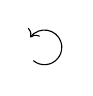
\begin{tikzpicture}
\draw[->] (-0.14,-0.17) arc (230:505:0.22);
\end{tikzpicture}
\end{adjustbox}

$\tau$-ф-я опред.
[зачёркнуто: \Unclear{GELFAND-P001102}{group-cancel}{при}]
только на таких; фактически на группе автом. $Gr$.

Тогда:
\begin{equation*}
\tau_W=\det(\omega_++a^{-1}b\omega_-)
\end{equation*}

\underline{Def.}\quad $W$ \underline{трансверсально} $(tr\ H_-)$ если $pr:W\to H_+$ изом. или
\begin{equation*}
W\cap H_-=\{0\}.
\end{equation*}

[Под «трансверсально» волнистое подчёркивание.]

Такое $W$ — график $\omega_-:H_+\to H_-$\qquad $\Rightarrow$ кан. выбор $\Rightarrow$

\begin{equation*}
\underline{\tau_W(1)=1}\qquad(\text{иначе }0)
\end{equation*}

[Под формулой волнистое подчёркивание.]

\underline{Замет.}\quad $\tau_W(g)=0\ \Leftrightarrow\ g^{-1}W$ не трансверс.

% В двух следующих формулах знак имеет три горизонтальные черты и косое перечёркивание; (745,2090)–(825,2170), (790,2390)–(860,2480); просмотр при 10×.
\underline{Лемма.}\quad $\forall W;\quad\tau_W\;
\begin{adjustbox}{max width=\linewidth}
\begin{tikzpicture}[baseline=-0.5ex]
\draw (0,0) -- (0.19,0);
\draw (0,0.05) -- (0.19,0.05);
\draw (0,0.10) -- (0.19,0.10);
\draw (0.05,-0.04) -- (0.15,0.15);
\end{tikzpicture}
\end{adjustbox}\;0.$

[Зачёркнуто: \Unclear{GELFAND-P001102}{nontransverse-cancel-first}{Нетр.}]
Нетрансвер. подпр-ва $W$ можно
\Incomplete{GELFAND-P001102}{nontransverse-cancel-second}{Зачёркнутое слово после «можно» не поддаётся надёжному чтению; различимо начало, похожее на «и», и два нижних выносных штриха.}
— аналог $\theta$-дивизора на якобиевом мн-жии кривой.

Точнее: $\tau_W(e^{xz})\;
\begin{adjustbox}{max width=\linewidth}
\begin{tikzpicture}[baseline=-0.5ex]
\draw (0,0) -- (0.19,0);
\draw (0,0.05) -- (0.19,0.05);
\draw (0,0.10) -- (0.19,0.10);
\draw (0.05,-0.04) -- (0.15,0.15);
\end{tikzpicture}
\end{adjustbox}\;0$

\begin{center}
\begin{adjustbox}{max width=\linewidth}
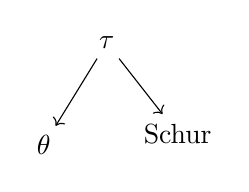
\begin{tikzpicture}
\node (tau) at (0,1.3) {$\tau$};
\node (theta) at (-0.8,0) {$\theta$};
\node (schur) at (0.9,0.15) {Schur};
\draw[->] (tau) -- (theta);
\draw[->] (tau) -- (schur);
\end{tikzpicture}
\end{adjustbox}
\end{center}

\underline{Schur.}\quad Рассм. спец. точки

[Перед $S$ зачёркнуто: \Unclear{GELFAND-P001102}{set-cancel}{H}]
\begin{equation*}
S=\{s_0<s_1<s_2<\ldots\},\qquad s_i=i;\quad i\gg0.
\end{equation*}

\begin{equation*}
\underline{-5\quad-3}\qquad0\quad1\quad2\quad
\begin{adjustbox}{max width=\linewidth}
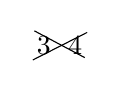
\begin{tikzpicture}[baseline=-0.5ex]
\node (three) at (0,0) {$3$};
\node (four) at (0.4,0) {$4$};
\draw (-0.14,-0.18) -- (0.55,0.17);
\draw (-0.12,0.19) -- (0.52,-0.15);
\end{tikzpicture}
\end{adjustbox}
\quad5\quad6\quad\ldots
\end{equation*}

\begin{equation*}
H_S=\{z^{s_i}\}_{s_i\in S}.
\end{equation*}

$\tau$-ф-я — ф-я Шура.

\SourcePage{GELFAND-P001103}{unlabelled}
Пусть есть \underline{разбиение}
\begin{equation*}
\nu=(\nu_1\geq\nu_2\geq\ldots),\qquad h_1,h_2,\ldots
\end{equation*}
$F_\nu(h)$ \Unclear{GELFAND-P001103}{top-schur-sign}{[густо обведённый знак: $=$ / тире]} ф-я Шура

\begin{equation*}
g(z)\in\Gamma_+,\qquad g^{-1}=1+h_1z+h_2z^2+\ldots
\end{equation*}
\begin{equation*}
\begin{aligned}
S&\leftrightarrow\nu\\
i-s_i&\leftrightarrow\nu_i
\end{aligned}
\end{equation*}
\underline{$\tau_W(g)=F_S(h)$}
[Подчёркнуто волнистой линией.]

\begin{center}— · —\end{center}
Вопрос: причем здесь $GL(n)$? ответа нет.
\begin{center}— · —\end{center}

\begin{equation*}
\tau_W(g)=\sum_S w^S F_S(g)
\end{equation*}
$w^S$ интерпрет. как плюккеровы коорд.
\Unclear{GELFAND-P001103}{schur-coefficient}{[В двух последних строках: $w^S$ / $\omega^S$; регистр $S$ не вполне ясен.]}

\begin{center}— · —\end{center}
\underline{Вложение конструкции Кричевера.}
[Подчёркнуто волнистой линией.]

$X$ — кривая (компактная компл.)
\begin{equation*}
D_\infty=\{|z|\geq 1\}
\end{equation*}
$D_\infty\subset X$

выб. вложение\qquad $S^1$ — граница

% Схема справа: исходные координаты (1410,1730,1755,1925), просмотр 5x.
\begin{center}
\begin{adjustbox}{max width=\linewidth}
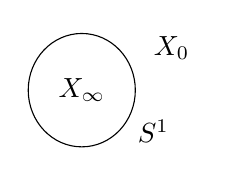
\begin{tikzpicture}
\draw (0,0) ellipse (0.68 and 0.72);
\node at (0,0) {$X_\infty$};
\node at (1.14,0.53) {$X_0$};
\node at (0.91,-0.52) {$S^1$};
\end{tikzpicture}
\end{adjustbox}
\end{center}
\begin{equation*}
X_0=X\setminus\operatorname{Int}X_\infty.
\end{equation*}

$\mathcal{L}$ — line bundle [под строкой: (голом.)]
(или: пучок без кручения ранга $1$, если $X$ с особ.)
[Под словами «без кручения»: $(t.f.)$.]

$\varphi=$ тривиализация $\mathcal{L}$ над $X_\infty$

сеч. над $S^1\leftrightarrow$ ф-и.

\underline{Строим точку на $Gr$:}
[Подчёркнуто волнистой линией.]
\begin{equation*}
W=\{f\in H\mid f\text{ — гран. знч. сечений }\mathcal{L}\text{ над }X_0\}.
\end{equation*}
[Над строкой, со знаком вставки перед «сечений»: (голом.).]

\underline{Утв.}\quad \underline{$W\in Gr$.}
[Под формулой волнистая линия.]
(\Unclear{GELFAND-P001103}{assertion-parenthetical}{полному с $\forall$ индексом})
\begin{equation*}
\operatorname{Ind}(W\longrightarrow H_+)=\chi(\mathcal{L})-1.
\end{equation*}

\underline{Замеч.}
Метод Кричевера [вставка над строкой: (постр. реш. KdV)] использует только $W$, а не кривую!

$\Rightarrow$ можно строить решения $\forall W$ !!

$\theta$-ф-я:
\begin{equation*}
\theta:H^1(X,O)\longrightarrow\mathbb{C}
\end{equation*}
\begin{equation*}
\tau_W:\Gamma_+\longrightarrow\mathbb{C}.
\end{equation*}
\SourcePage{GELFAND-P001104}{49}
Связь --- ?
\begin{equation*}
\begin{adjustbox}{max width=\linewidth}
\begin{tikzcd}
\Gamma_+ \\
V \arrow[u,"\exp","\simeq"']
\end{tikzcd}
\end{adjustbox}
\qquad (\text{аналитич. ф-и }f\colon D_0\longrightarrow\mathbb C).
\end{equation*}
\begin{equation*}
\begin{adjustbox}{max width=\linewidth}
\begin{tikzcd}
& V \arrow[d,"\underline{\text{на}}"] \\
\theta\colon & H^1(X,O) \arrow[r] & \mathbb C
\end{tikzcd}
\end{adjustbox}
\qquad
\begin{adjustbox}{max width=\linewidth}
\begin{tikzcd}
f \arrow[d] \\
\bar f\in H^1(X,O)
\end{tikzcd}
\end{adjustbox}
\end{equation*}
\SourceFigure{GELFAND-P001104}{diagram-01}{Три вложенных замкнутых контура с поперечными штрихами; слева $f$, справа $X_0$, снизу $U_\infty$, $U_0$; знак внутри внутреннего контура требует проверки.}

\Unclear{GELFAND-P001104}{cocycle-inclusion}{$f\in V\in Z^1(U,O)$}

(предст. коциклом Чеха $=$ ф-я в окр. окружности).
\begin{equation*}
\widetilde\tau_W(f)=e^{\alpha_{W,0}(f)+Q(f)}\theta(\bar f-\beta_W)
\end{equation*}
$Q$ зав. только от $(X,D_\infty)$.

\underline{Вопрос И.М.Г.} Построить теорию интегрир., связ. с $\theta$-ф-ей $\forall$ абелевых мн-зий

(здесь возникают [зачеркнуто: \Unclear{GELFAND-P001104}{cancel-before-only}{неразборчивый знак}] только якобианы алгебр. кривых)

\begin{center}--- $\cdot$ ---\end{center}
\underline{Ф-ла, связывающая $\tau$-ф-ю с $\Psi$-ф-ей Baker'a} (--Ахиезера)

[Под именем Baker: (1928 г.)]

$W\in Gr$; $z\in S^1$. Характериз. св-вами:
\begin{equation*}
\text{(i)}\quad \Psi_W(g,z)=g(z)\underbrace{\left(1+\sum_{i=1}^{\infty}a_i(g)z^{-i}\right)}_{\widetilde\Psi(g,z)}
\end{equation*}
\begin{equation*}
\text{(ii)}\quad \Psi(g,\cdot)\in W,\quad \forall g\in\Gamma_+.
\end{equation*}
\underline{Предл.} $\forall W$, $\exists!$ такая $\Psi_W$ [зачеркнуто: \Unclear{GELFAND-P001104}{cancel-after-psi}{для любого (?)}].

Если $g^{-1}W\cap H_-=\{0\}$, то значение строится:
[зачеркнуто: \Unclear{GELFAND-P001104}{cancel-before-preimage}{неразборчивый знак}] прообразу $1$ при изом.
\begin{equation*}
g^{-1}W\overset{\simeq}{\longrightarrow}H_+
\end{equation*}
[Зачеркнута строка: \Unclear{GELFAND-P001104}{cancel-transverse}{$g^{-1}W$ трансвер. (?)}.]

\underline{Предл.} $\exists!$ $\Psi_W(g,z)$ --- мероморфная на $\Gamma_+$.

Д-во как в случае кривых

(там использ. $\theta$-ф-я, а здесь $\tau$-ф-я)

\begin{center}--- $\cdot$ ---\end{center}
$|\zeta|>1\quad\Rightarrow$ определим \Unclear{GELFAND-P001104}{auxiliary-group-element}{$q_\zeta\in\Gamma_+$, $q_\zeta(z)=1-z/\zeta$}.

\underline{Предл.} (\Unclear{GELFAND-P001104}{last-proposition-abbreviation}{яв. ф-ла (?)}). При $|\zeta|>1$
\begin{equation*}
\widetilde\Psi_W(g,\zeta)=\frac{\tau_W(gq_\zeta)}{\tau_W(g)}
\end{equation*}

\SourcePage{GELFAND-P001105}{unlabelled}
Или:

запишем в виде $\exp$ и будем всё рассм. как ф-и от $t$ (беск. число)

\Unclear{GELFAND-P001105}{tau-shift-slash}{$\widetilde\Psi_W(t,z)=\dfrac{\tau_W(t_1-1/z,\ t_2-1/2z^2,\ldots)}{\tau_W(t)}$}
\begin{equation*}
\left(g=e^{\sum_1^{\infty}t_i z^i}\right).
\end{equation*}
Или:
\begin{equation*}
\Psi=\frac{(\text{верш. оператор})\tau}{\tau}
\end{equation*}
\begin{equation*}
\underline{\text{верш. опер.}}=e^{\sum t_i z^i}e^{-\sum(\partial/\partial t_i)z^{-i}/i}
\end{equation*}
\underline{Следствие:} $a_i(g)$ мероморфны на $\Gamma_+$.

\begin{center}--- $\cdot$ ---\end{center}
Связь с нелин. ур-ями --- как у Кричевера!

\begin{center}--- $\cdot$ ---\end{center}
[Зачеркнуто: \Unclear{GELFAND-P001105}{cancelled-hierarchy-heading}{В… [остальное неразборчиво]}]
\underline{$\forall W$ имеется беск. иерархия ур-ий.}

\begin{center}--- $\cdot$ ---\end{center}
\begin{equation*}
\begin{adjustbox}{max width=\linewidth}
\begin{tikzcd}
Gr \arrow[d] \\
\{\text{решение КП-иерархии}\}
\end{tikzcd}
\end{adjustbox}
\qquad D=\partial/\partial x;\qquad Q=D+\sum_1^{\infty}q_i D^{-i}
\end{equation*}
\begin{equation*}
\frac{\partial Q}{\partial t_r}=[(Q^r)_+,Q]
\end{equation*}
[От $(Q^r)_+$ черта к подписи: дифф. часть $Q^r$.]

Если $Q^n=L$ дифференциальный, то получ. сист. Г.--Д.:
\begin{equation*}
\frac{\partial L}{\partial t_r}=[L_+^{r/n},L]
\end{equation*}
и обратно, если $L$ дифф. $Q=[L^{1/n}]$, то получ.
[зачеркнуто: \Unclear{GELFAND-P001105}{cancelled-before-equation}{неразборчивый знак}] ур-е, вып. выше:
\begin{equation*}
\begin{adjustbox}{max width=\linewidth}
\begin{tikzcd}
Gr^{(n)}=\{W\in Gr\mid z^nW\subset W\} \arrow[d] \\
\{L=D^n+\ldots\}
\end{tikzcd}
\end{adjustbox}
\ ;\quad L\Psi_W=z^n\Psi_W
\end{equation*}
При этом:
\begin{equation*}
g=e^{xz+t_2z^2+\ldots}
\end{equation*}
Полюса --- ? Из утв. о полюсах:

в частности $L(x,t_2^0,t_3^0,\ldots)$ имеет лишь \underline{регул. особ. точки.}
\begin{equation*}
\underline{n=2}:\qquad \fbox{$u=D^2\log\tau$}
\end{equation*}
$(L=\dfrac{d^2}{dx^2}+\ldots)$

\begin{center}--- $\cdot$ ---\end{center}

\SourcePage{GELFAND-P001106}{50}
Расслоение:

\begin{center}
\begin{adjustbox}{max width=\linewidth}
\begin{tikzpicture}
\node (det) at (0,1) {$Det$};
\node (gr) at (0,-0.8) {$Gr$};
\draw[->] (det) -- (gr);
\node[align=left,anchor=west] at (1.6,0.35) {«слой над $W$ равен $\bigwedge^{\frac12\infty}W$»};
\draw[->] (1.4,0.25) -- (0.45,0.25);
\end{tikzpicture}
\end{adjustbox}
\end{center}
\begin{equation*}
\dim W=\frac12\infty\qquad(\text{старшая внешн. степ.})
\end{equation*}
[Под правой пометой зачеркнуто: \Unclear{GELFAND-P001106}{cancelled-top-caption}{1-мерное (?)}.]

1-мерное линейн. рассл.
\begin{equation*}
\begin{adjustbox}{max width=\linewidth}
\begin{tikzcd}
\omega \arrow[d] \\
W=\operatorname{Im}\omega
\end{tikzcd}
\end{adjustbox}
\qquad
\begin{adjustbox}{max width=\linewidth}
\begin{tikzcd}
{\mathcal P=\left\{\omega\colon H_+\hookrightarrow H\ \middle|\ 
\begin{aligned}\omega_+&=1+\text{nuclear}\\\omega_-&\quad\text{compact}\end{aligned}\right.}
\arrow[d] \\
Gr
\end{tikzcd}
\end{adjustbox}
\end{equation*}
\begin{equation*}
\mathcal T=\left\{\underset{\text{обрат.}}{t}\colon
\begin{adjustbox}{max width=\linewidth}
\begin{tikzcd}H_+\arrow[loop right]\end{tikzcd}
\end{adjustbox}
\ \middle|\ t=1+\text{nucl.}\right\}
\end{equation*}
\begin{equation*}
\det\colon\mathcal T\longrightarrow\mathbb C^*
\end{equation*}
\begin{equation*}
Det=\mathcal P\underset{\mathcal T}{\times}\mathbb C.
\end{equation*}
\begin{equation*}
GL_1(H)=\left\{\begin{pmatrix}a&b\\c&d\end{pmatrix}\quad
\begin{matrix}a\\d\end{matrix}\ \middle|\ 
\begin{matrix}\text{Fred}\\\operatorname{ind}=0\end{matrix},\quad b,c\text{ --- nuclear}\right\}.
\end{equation*}
\Unclear{GELFAND-P001106}{action-word-correction}{Действие [исправление в середине слова]} её на $Gr$ поднимем до действия на $Det$.
\begin{equation*}
\mathcal E\subset GL_1(H)\times GL(H_+)
\end{equation*}
\begin{equation*}
\mathcal E=\left\{(g,q)\ \middle|\ aq^{-1}=1+\text{nuclear};\quad
 g=\begin{pmatrix}a&b\\c&d\end{pmatrix}\right\}.
\end{equation*}
\Unclear{GELFAND-P001106}{extension-initial-sign}{$1\longrightarrow\mathcal T\longrightarrow\mathcal E\longrightarrow GL_1(H)$}

\underline{Утв.:} расширение нетривиально.

В конечномерном случае получ. тривиальное расширение.

Действие $\mathcal E$ на $Det$:
\begin{equation*}
(g,q)(\omega,\lambda)=(g\omega q^{-1},\lambda)
\qquad\text{из предст.}\quad Det=\mathcal P\underset{\mathcal T}{\times}\mathbb C.
\end{equation*}
\Unclear{GELFAND-P001106}{kernel-notation}{$\mathcal T_0=\ker\det\mathcal T\longrightarrow1$}

[Зачеркнуто: \Unclear{GELFAND-P001106}{cancelled-before-elements}{неразборчивый знак}] Элем. $\mathcal T_0$ (их образ в $\mathcal E$) действуют тривиально.
$\Rightarrow$ действует $\mathcal E/\mathcal T_0$.
\begin{equation*}
1\longrightarrow\mathbb C^*\longrightarrow
\underset{\mathcal E/\mathcal T_0}{\underset{\Vert}{\widehat{GL}_1}}
\longrightarrow GL_1(H)\longrightarrow 1
\end{equation*}
[Перед конечной единицей зачеркнуто: \Unclear{GELFAND-P001106}{cancelled-terminal-sign}{0 (?)}.]

\SourcePage{GELFAND-P001107}{unlabelled}
\begin{equation*}
\begin{adjustbox}{max width=\linewidth}
\begin{tikzcd}
\mathrm{MkdV}\arrow[d]\\\mathrm{KdV}
\end{tikzcd}
\end{adjustbox}
\qquad
\begin{adjustbox}{max width=\linewidth}
\begin{tikzcd}
v_t=v_{xxx}-6v^2v_x\arrow[d,"\mu"']\\
u_t=u_{xxx}+6uu_x
\end{tikzcd}
\end{adjustbox}
\end{equation*}
\begin{equation*}
\underline{u=v_x-v^2}
\end{equation*}
[Зачеркнуто: \Unclear{GELFAND-P001107}{cancelled-replaced-word}{Рассмотрим (?)}; над ним: Недавно] это [вставлено: понято] лучше.

$\mathrm{KdV}$ связ. с
\begin{equation*}
\underbrace{D^2+u=(D-v)(D+v)}_{(u=v_x-v^2)}
\end{equation*}
обобщение пр. части:
\begin{equation*}
D^n+u_{n-2}D^{n-2}+\ldots+u_0=(D-v_{n-1})\ldots(D-v_0)
\end{equation*}
[У первого $D$ в правой части зачеркнуто: \Unclear{GELFAND-P001107}{cancelled-factor-subscript}{неразборчивый нижний знак}.]
\begin{equation*}
v\longmapsto u
\end{equation*}
\underline{обобщ. преобр. Миуры.}

[Зачеркнуто: \Unclear{GELFAND-P001107}{cancelled-before-drinfeld}{неразборчивый знак}] Дринфельд, Соколов обобщили на $\forall$ простую гр. вместо $SL_n$.

Соответствие не вз.-однозначн. (дифф. ур-е)

[Под скобками: надо реш. уже при $n=2$.]
\begin{equation*}
n=2\quad\Rightarrow\quad\forall u\text{ есть 1-пар. сем-во }v.
\end{equation*}
$u_i(x)$ --- аналит.
\begin{equation*}
\{\text{Аналит. решения}\}=\{\text{клетка}\}\simeq\mathbb C^N
\end{equation*}
\begin{equation*}
\left\{\begin{gathered}\text{мероморфные реш.}\\\text{в окр. точки}\end{gathered}\right\}
=\{\text{мн-ие флагов }SL(n)/B\}
\end{equation*}
$\forall n$ есть сист. нелин. дифф. ур-ий; решения имеют структуру мн-зия флагов.

Осн. сложность:
\begin{equation*}
\begin{adjustbox}{max width=\linewidth}
\begin{tikzcd}\mathrm{MkdV}\arrow[d]\\\mathrm{KdV}\end{tikzcd}
\end{adjustbox}
\quad\text{--- не отобр. Галуа (нет группы, действ. на слоях).}
\end{equation*}
Рассм. дифф. поле, порожденное $v_0,\ldots,v_{n-1}$.

\begin{center}
\begin{adjustbox}{max width=\linewidth}
\begin{tikzpicture}
\node at (0,0) {$\{\text{коэффициенты}\}\subset\{\text{корни}\}\underset{B}{\subset}\{\text{решения}\}$};
\draw (-2.3,-0.4) .. controls (-1.9,-1.4) and (1.2,-1.3) .. (2.7,-0.45);
\node at (0,-0.85) {$SL(n)$};
\node[align=center] at (0,-1.55) {аналог\\гр. Галуа};
\end{tikzpicture}
\end{adjustbox}
\end{center}

\SourcePage{GELFAND-P001108}{unlabelled}
% Верхняя большая часть кадра не содержит рукописного текста; запись начинается внизу.
\underline{11/IV-83 г.}\qquad\underline{Сем. Гельфанда}

\underline{\underline{Wilson.}}
\begin{equation*}
Q=D+\sum_1^{\infty}q_iD^{-i},\qquad L\text{ --- дифф.}\quad\Rightarrow
\end{equation*}
\begin{equation*}
\frac{\partial Q}{\partial t_r}=[Q_+^r,Q]
\quad\Longleftrightarrow\quad
L_{t_r}=[L_+^{r/n},L]\qquad(\text{Г.--Д.})
\end{equation*}
[После первой скобки: \Unclear{GELFAND-P001108}{cancelled-after-commutator}{неразборчивый зачеркнутый знак}. В первом аргументе второго коммутатора: \Unclear{GELFAND-P001108}{retouched-l-in-commutator}{$L$ [обведено/исправлено]}.]
\begin{equation*}
2\text{ переменные }t_2,t_3\quad\Rightarrow\quad
2q_1(x,\underset{y}{t_2},\underset{t}{t_3})
\text{ --- решение К.-П.}\quad\Rightarrow\quad\text{универс. КП}
\end{equation*}

\SourcePage{GELFAND-P001109}{unlabelled}
\underline{В. Гинзбург.}

о работах:

1) \Unclear{GELFAND-P001109}{first-listed-surname}{Дюйстермаат (?)}, Хекман (Inventiones)

2) Атия, Ботт

3) Виттен

4) М. Вернь, N. Conze

(\Unclear{GELFAND-P001109}{pupils-parenthesis}{ученицы Диксмье (?)})

[Справа от списка, за вертикальной чертой: Березин, Гельфанд (5 т. тр. ММО). Под скобками: 1956.]

\underline{Д.-Х.}
\begin{equation*}
\text{(1)}\qquad\int_M e^{iH}=\sum_j\frac{\operatorname{vol}(M_j)e^{iH(M_j)}}{\lambda_j}
\end{equation*}
$M$ --- комп. мн-ие, симплектическое.

$H$ --- ф-я на $M$; условие на неё: Инт. кривые [вставлено: гам.] поля
[зачеркнуто: \Unclear{GELFAND-P001109}{cancelled-field-symbol}{неразборчивое обозначение}] $\xi_H$ замкнуты.

[Зачеркнута строка: \Unclear{GELFAND-P001109}{cancelled-periodic-flow-line}{(точнее фаз. поток его периодичен (?))}.]

(фаз. поток компактен)

[Ниже приписано и подчеркнуто: периодичен (?)]

$M_j$ --- критич. мн-зия ф-и $H$ (критич. уровни) --- они подмн-зия

[Под «критич. уровни»: где $dH=0$. Справа: (следует из комп. потока).]

$\operatorname{vol}M_j$ --- объём отн. индуц. симпл. структуры.

$H$ постоянна на $M_j$ $\Rightarrow$ $H(M_j)$ --- её значение.

$\lambda_j$ опр. действием [вставлено: $\xi_H$] в
$\left(T_xM/T_xM_j\right)$\qquad($T_xM_j$ сохран.)

Действие $\xi_H$ кососимметрическое: $\lambda_j$ --- его пфаффиан $(=\sqrt{\det})$.

Действие эквивал. линейному, а для лин. всё хорошо.

\underline{Вопрос И.М.Г.:} не использованы ещё соб. значения стац. действия.

Идея док-ва:
\begin{equation*}
\int_M e^{itH}\mu\quad\text{--- пр. Фурье --- выч. по методу стац. фазы --- получ.}
\end{equation*}
[Под последними словами: точн. ответ]
\begin{equation*}
\int\ \text{по пов. уровня}\quad\text{---}\quad\underline{\text{кусочный многочлен.}}
\end{equation*}
$\mu$ из симплект. формы $\Rightarrow$ всё пишется в подход. лок. коорд.

Дост. док., что \underline{симпл. форма} --- многочлен (на самом деле линейная ф-я)
\begin{equation*}
\mu\quad
\begin{adjustbox}{max width=\linewidth}
\begin{tikzcd}M\arrow[d,"f"]\\\mathbb R\end{tikzcd}
\end{adjustbox}
\qquad\text{Прямой образ меры }\mu\text{ на }\mathbb R\text{ --- многочлен на }\mathbb R.
\end{equation*}

\SourcePage{GELFAND-P001110}{58}
$\left.\begin{gathered}\underline{\text{А.-Б.}}\\\text{и др.}\end{gathered}\right\}$
$M$ --- компактное мн-зие, $G$ --- комп. гр. Ли, действ. на $M$.
\begin{equation*}
H_G^*(M)\text{ --- ?}
\end{equation*}
(когомологии)
\begin{equation*}
\begin{adjustbox}{max width=\linewidth}
\begin{tikzcd}EG\arrow[d,"G"]\\BG\end{tikzcd}
\end{adjustbox}
\quad\text{--- универс. рассл.}
\end{equation*}
[Зачеркнуто: \Unclear{GELFAND-P001110}{cancelled-universal-bundle-word}{неразборчивое слово}] соотв. $G$; $EG$ стягиваемо.

Рассм. $EG\underset{G}{\times}M$
\begin{equation*}
H_G^*(M)\overset{\mathrm{def}}=H^*(EG\underset{G}{\times}M)\qquad(\text{Борель})
\end{equation*}
$EG\underset{G}{\times}M$ --- рассл. над $BG$ со слоем [зачеркнуто: \Unclear{GELFAND-P001110}{cancelled-before-fiber-m}{неразборчивый знак}] $M$
\begin{equation*}
H^*(EG\underset{G}{\times}M)\text{ --- модуль над }H^*(BG)\qquad(\text{многочлены!})
\end{equation*}
[От $H^*(BG)$ черта к подписи: кольцо многочленов.]

будет $G=S^1$ и тогда $H^*(BG)$ --- кольцо мног. от 1-й переменной.

\underline{Теор. о локализации.}

$M^G$ --- мн-во неподв. точек действия $G$.
\begin{equation*}
\text{(1)}\qquad H_G^*(M)\longrightarrow H_G^*(M^G)
\end{equation*}
на $M^G$ действие трив. $\Rightarrow$
\begin{equation*}
H_G^*(M^G)=\underbrace{H^*(BG)\otimes
\underbrace{H^*(M^G)}_{\substack{\text{обычные}\\\text{когом.}}}}
_{\substack{\text{умн., чтобы получить}\\H^*(BG)\text{-модуль.}}}
\end{equation*}
[Под $M$ слева зачеркнуто: \Unclear{GELFAND-P001110}{cancelled-m-subscript}{неразборчивый нижний знак}.]

\underline{Теор.}

Если локализовать по [зачеркнуто: \Unclear{GELFAND-P001110}{replaced-coefficient-word}{всему (?)}; над ним: кольцу] коэффициентов,
то получ. изоморфизм [зачеркнуто: \Unclear{GELFAND-P001110}{cancelled-after-isomorphism}{неразборчивый знак}]
\begin{equation*}
\text{(2)}\qquad\text{лок.}\bigl(H_G^*(M)\bigr)
\overset{\sim}{\longrightarrow}\text{лок.}\bigl(H_G^*(M^G)\bigr)
\end{equation*}
(т.е. заменить [вставлено: $H^*(BG)$] на поле [зачеркнуто: \Unclear{GELFAND-P001110}{cancelled-before-ratios}{неразборчивое слово или знак}] отношений).

В $K$-теории --- Атия, Сегал.

В когомол. --- Quillen.

\underline{А.-Б.}\qquad\underline{Интерпретация $H_G^*(M)$ через дифф. формы}

Теор. локализации (2) тогда эквив. теор. Виттена о киллинговом поле.
\begin{equation*}
G=S^1\qquad
\begin{adjustbox}{max width=\linewidth}
\begin{tikzcd}
EG\arrow[d]&={} &S^\infty\arrow[d]&\text{(беск.-мерн. сфера)}\\
BG&={} &\mathbb CP^\infty
\end{tikzcd}
\end{adjustbox}
\end{equation*}
\begin{equation*}
H^*(BG)=\mathbb Q[u],\quad\operatorname{deg}u=2.
\end{equation*}

\SourcePage{GELFAND-P001111}{unlabelled}
$\xi$ --- векторное поле, опр. действие $S^1$.
\begin{equation*}
\Omega_M\otimes\mathbb C[u]\qquad(\text{чтобы получить }\mathbb C[u]\text{-модуль})
\end{equation*}
[От $\Omega_M$ черта к подписи: дифф. формы на $M$.]

\underline{Дифференциал} в $\Omega_M\otimes\mathbb C[u]$:

[Справа, отмечено двойной вертикальной чертой: \underline{Надо:} написать формы на $EG\underset{G}{\times}M$ и из них исходить. (с обычным $d$)]
\begin{equation*}
\text{(3)}\qquad d_1\omega=d\omega+u\cdot i_\xi\omega
\qquad(\text{подкрутка как у Виттена})
\end{equation*}
Степени согласованы!

\underline{Теор.}

(4) Когомологии\quad \Unclear{GELFAND-P001111}{unrestricted-complex-in-four}{$H(\Omega_M\otimes\mathbb C[u],d_1)\simeq H_G^*(M)$}.

Из ф-лы гомотопии
\begin{equation*}
L_\xi=d\circ i_\xi+i_\xi\circ d
\end{equation*}
следует, что

[Зачеркнуто: от]

\Unclear{GELFAND-P001111}{square-of-differential}{$d_1^2=u^2L_\xi$}

Отсюда если $d_1\omega=0$, то $\omega$ инвариантна, т.е. $L_\xi\omega=0$.

\underline{Подкрут. формы:} [зачеркнуто: \Unclear{GELFAND-P001111}{cancelled-before-xi-invariant}{неразборчивый знак}] $\xi$-инвариантные!! (с самого начала).
\begin{equation*}
\Omega^G=\Omega_M^G\otimes\mathbb C[u],\qquad\Omega_M^G\text{ --- инвар. формы на }M;
\end{equation*}
\underline{А. Гончаров:} это $\sim$ констр. Черна-Вейля хар. классов по связностям.

\underline{Следствие локализации:} $u$ стирается.

(5) \underline{Теор.}
\begin{equation*}
\text{Когомологии}\quad
\left(\Omega_M^G,\ d_1=d+i_\xi\right)
\overset{\sim}{\longrightarrow}H^*(M^G).
\end{equation*}
\underline{Зад. И.М.Г.} Сформулир. то же без $G$ на языке двойного рассл.
\begin{equation*}
\begin{adjustbox}{max width=\linewidth}
\begin{tikzcd}
&EG\underset{G}{\times}M\arrow[dl]\arrow[dr]&\\
BG&&M/G
\end{tikzcd}
\end{adjustbox}
\end{equation*}
\begin{center}--- $\cdot$ ---\end{center}
Слева в (5) нет деления на степени --- только чётности.

Ограничиваем на $M^G$: $i_\xi=0$ там и получим обычное $d$!

Это и есть отобр. в (5)

Виттен: число неподв. точек киллингова поля --- пр. часть

[Ниже:] лв. часть --- супердифференциалы

\SourcePage{GELFAND-P001112}{59}
Теперь Раб. М. Вернь (её правильное прочтение):

[Приписка под именем, соединённая с верхней строкой штрихами:]
у неё интегралы (\Unclear{GELFAND-P001112}{top-integrals-adjective}{сложные? / лишние?})

\underline{Лемма} (основная). Если неподв. точек нет, то когомологии слева $=0$.
\begin{equation*}
M^G=0\quad\Longrightarrow\quad
H^*(\Omega_M^G,d_1=d+i_\xi)=0.
\end{equation*}
М. Вернь: явно написала, от чего граница рассм. цикл:

Общее рассужд.: выкид. неподв. точки и делаем то же самое.

\begin{center}
\begin{adjustbox}{max width=\linewidth}
\begin{tikzpicture}
\node at (-0.6,0) {$M$};
\draw (0,-0.45) .. controls (0.3,-0.2) and (0.3,0.25) .. (0,0.45);
\draw (0.35,-0.45) .. controls (0.65,-0.2) and (0.65,0.25) .. (0.35,0.45);
\draw (0.75,-0.5) .. controls (1.05,-0.2) and (1.05,0.25) .. (0.75,0.45);
\draw (1.22,-0.45) .. controls (1.52,-0.2) and (1.52,0.25) .. (1.22,0.45);
\draw (1.65,-0.45) .. controls (1.95,-0.2) and (1.95,0.25) .. (1.65,0.45);
\draw (2.1,-0.5) .. controls (2.4,-0.2) and (2.4,0.25) .. (2.1,0.42);
\draw (2.45,-0.56) .. controls (2.8,-0.2) and (2.8,0.25) .. (2.45,0.42);
\draw (2.9,-0.63) .. controls (3.35,-0.22) and (3.2,0.3) .. (2.9,0.45);
\node[anchor=west] at (3.6,0) {--- окр. $S^1$ действ. без неподв. точек.};
\end{tikzpicture}
\end{adjustbox}
\end{center}
\begin{equation*}
\alpha=d\varphi\qquad(1\text{-форма})\tag{6}
\end{equation*}
\underline{Св-ва} (желание)
\begin{align}
L_\xi\alpha&=0\tag{7}\\
i_\xi\alpha&=1\tag{8}\\
d\alpha&=0.\tag{9}
\end{align}
\begin{equation*}
\text{Усл. (7), (8) удовл. можно}\qquad
\alpha(\cdot)=\frac{\langle\xi,\cdot\rangle}{\langle\xi,\xi\rangle}.\tag{*}
\end{equation*}
(9) не нужно, т.к. раб. с $d_1$. Перепишем (9):
\begin{equation*}
d_1\alpha=1\qquad\text{(в силу (8))}.\tag{10}
\end{equation*}
$d\alpha=1$ невозможно.

Изгот. форму $\beta$:

[Перед левой чертой зачеркнуто: \Unclear{GELFAND-P001112}{lower-before-equation-11}{неразборчивый знак}]
\begin{equation*}
\begin{array}{r|l|l}
(11)&L_\xi\beta=0&\underline{\text{это достаточно}}\\
(12)&d_1\beta=1&
\end{array}
\end{equation*}
\begin{equation*}
\text{М. Вернь:}\qquad
\beta=\alpha(1+d\alpha)^{-1}
=\alpha(1-d\alpha+d\alpha\wedge d\alpha-\ldots),\tag{13}
\end{equation*}
где $\alpha$ --- ф-ла (*). Всё легко проверяется.

Придумать: нач. с $\alpha$ и по теории возмущений.

Имеем тождество:
\begin{equation*}
\omega=d_1(\beta\wedge\omega)+\beta\wedge d_1\omega,\tag{14}
\end{equation*}
отсюда если $d_1\omega=0$, то $\omega=d_1(\beta\wedge\omega)$.

\underline{Вычисление интеграла по $M$} (от $d_1$-замкн. формы):
$\forall$ такой интеграл сводится к интегр. по мн-ву неподв. точек.
По теор. Стокса! ---

--- изв., что $\omega=d_1(\beta\wedge\omega)$; асимптотику надо вычислить при прибл. к неподв. точкам.

\SourcePage{GELFAND-P001113}{unlabelled}
% Верхняя часть кадра до начала записи пуста. Внутренней метки листа не видно.
\underline{\underline{18/IV-83 г.}}\qquad\underline{Сем. Гельфанда}.

Разобрать раб. \underline{Левинсона} о $\zeta$-ф-и. (упростил гип. Римана)

\underline{\underline{В. Гинзбург.}}

$M$ --- симплект. компактное мн-зие.

Пусть на нём действует тор $\mathbb T^n$.

Отобр. момента\quad $M\overset{\mu}{\longrightarrow}t^*$

[Справа, в рамке:]
\begin{flushright}
\fbox{\parbox{6cm}{Должно быть дано предст. $t$ в алгебру ф-й на $M$ со скобкой $\{\ \}$ Пуассона.}}
\end{flushright}
\begin{equation*}
\begin{adjustbox}{max width=\linewidth}
\begin{tikzcd}[column sep=small,row sep=small]
\mu(m): & X\arrow[r] & H_X(m)\\
& t\arrow[u] &
\end{tikzcd}
\end{adjustbox}
\end{equation*}
$H_X$ --- ф-я гамильт., отвечающая эл. $X$ (как векторному полю на $M$)

(заданы $H_X$ для каждого $X$).

[На левом поле: !!; ниже: \Unclear{GELFAND-P001113}{left-margin-below-exclamations}{к.? / н.?}]

(1) \underline{Утв.}\quad $\mu(M)$ --- \underline{выпуклый многогранник}.

[Справа:]
(Атья-Ботт и Гийемин-Стернберг независимо)

Есть ещё компл. случай

(Дюйстермаат и [зачеркнуто: \Unclear{GELFAND-P001113}{middle-before-heckman}{неразборчивое начало слова}] Хекман --- ф-я, опр. на прошлом докл. --- кус. полином на $\mu(M)$).

\underline{Грани} (переход) --- где $d\mu$ вырождается.

Они плоскости: применяем к мн-зиям вырожд., где ранг падает на несколько единиц.

\underline{\underline{А. Бейлинсон.}}

\underline{Значения в целых точках $\zeta$-функций многообразий над числ. полями.}

1. Формулир. с точн. до умножения на [зачеркнуто: \Unclear{GELFAND-P001113}{lower-before-rational-number}{$Q$?}] рац. число $\ne0$ (элемент $\mathbb Q^*$)

2. Точные формулир.

Гипотеза \Unclear{GELFAND-P001113}{lower-conjecture-names}{Бёрча? — Суиннертона?} $=$ Дайера

$X/\mathbb Q$ --- гладкая кривая;\quad $\zeta(x,s)$ --- её $\zeta$-функция

[Под словами «гладкая кривая» двумя строками:]

(проективная)

рациональная

$X/\mathbb Z$ \Unclear{GELFAND-P001113}{bottom-reduction-abbreviation}{неразборчивое сокращение (уд-л-щая?)} невырожд. редукции по любому $p$

(ур-я выбраны дост. хорошие).

[Справа от последней строки:]
(если средуцируем ур-я $\operatorname{mod}p$, то получим снова гладкую кривую)
\SourcePage{GELFAND-P001114}{unlabelled}
\begin{equation*}
 (1)\quad \zeta(X,s):=\prod_p\zeta(X\otimes\mathbb Z/p\mathbb Z,s).
\end{equation*}
Здесь
\begin{equation*}
 (2)\quad \zeta(X\otimes\mathbb Z/p\mathbb Z,s):=
 \sum\underbrace{X(\mathbb F_{p^n})}_{\substack{\text{число}\text{ точек над}\\\mathbb F_{p^n}}}p^{-ns}.
\end{equation*}
\Unclear{GELFAND-P001114}{local-zeta-formula}{[Формула (2) записана именно как сумма; дополнительные множители не дописаны.]}

обычная $\zeta$-ф-я
\begin{equation*}
 \prod\frac{1}{1-p^{-s}}=\prod(1+p^{-s}+p^{-2s}+\ldots)
\end{equation*}
Здесь $X$ --- точка (т.е. $\mathbb Q$).

\underline{Вопр. И.М.Г.}
\begin{equation*}
 \prod_p\sum a_n(p)p^{-ns}
\end{equation*}
какие разумные $a_n(p)$
(они $\equiv1$ для обычной $\zeta$-ф-и).

\underline{Гипотеза Вейля (для кривой доказана):}
получ. [зачеркнуто: \Unclear{GELFAND-P001114}{weil-cancelled}{неразборчиво}] рац. ф-я от $p^{-s}$
\Incomplete{GELFAND-P001114}{weil-cancelled-loss}{Зачёркнутое слово между «получ.» и «рац. ф-я» не восстановлено; соседние читаемые слова сохранены.}
\begin{equation*}
 \frac{\prod(1-\alpha_i p^{-s})}{\prod(1-\beta_j p^{-s})}
\end{equation*}
\underline{Нули при}
\Unclear{GELFAND-P001114}{weil-zero-exponent}{$\operatorname{Re}z=p^{1/2}$ или $p^{n/2}$; числитель показателя переправлен}.

\underline{Для кривых даже не док. факт. аналитич. продолжения $\zeta(X,s)$}.
(Над конечн. полями --- полная информация [вставлено снизу: есть]).
[Справа: Сходится при $\operatorname{Re}s>2$.]
--- вопрос согласования при различных $p$.

\underline{Известно:} $\zeta$-ф-и Ланглэндса продолжаются.
[Зачеркнуто: \Unclear{GELFAND-P001114}{strong-conjecture-cancelled}{неразборчивое слово}.]
\Incomplete{GELFAND-P001114}{strong-conjecture-cancelled-loss}{Зачёркнутое короткое слово не восстановлено; начальный Б-подобный штрих остаётся лишь фрагментом.}
\underline{Гипотеза (сильная):} совпадают эти 2 кл. $\zeta$-ф-й.
[Разделитель: две короткие горизонтальные черты с точкой между ними.]
[Между записями слева зачеркнут знак:
\Unclear{GELFAND-P001114}{between-talks-mark}{неразборчиво}.]

\underline{Водзицки М.} Какие
[зачеркнуто: \Unclear{GELFAND-P001114}{wodzicki-cancelled}{ряды?}]
\Incomplete{GELFAND-P001114}{wodzicki-cancelled-loss}{Зачёркнутое слово не восстановлено полностью; «ряды?» и видимые нижние штрихи сохранены как неопределённое чтение.}
$\zeta$-ф-и считаются?

\underline{Шинтани:} $\zeta$-ф-я Дедекинда
[зачеркнут знак: \Unclear{GELFAND-P001114}{shintani-cancelled}{неразборчиво}]
свод. к $\zeta$-ф-ям ПДО
\begin{equation*}
 \zeta_{K/\mathbb Q}(s)=\sum N\mathfrak a^{-s}=\sum a_n n^{-s}.
\end{equation*}
\Unclear{GELFAND-P001114}{dedekind-ideal}{[Знак после $N$: $\mathfrak a$ или $a$; сильно обведен.]}
Выраж. через ПДО на торе (с пост. коэффициентами).

[Разделитель: две короткие горизонтальные черты с точкой между ними.]

\underline{Б.}\quad \underline{Гипотеза Берча --- Суинн.-Дайера}

[На левом поле: $X$ --- кривая.]

1) Аналит. продолжается.

2) функц. ур-е
\begin{equation*}
 (2\pi)^{-s}\Gamma(s)\zeta(X,s)\quad
 \text{симметр. относит. замены }s\to2-s
\end{equation*}
[Справа:]
\begin{adjustbox}{max width=\linewidth}
\begin{tikzpicture}[x=0.6cm,y=0.6cm]
\draw (0,-1) -- (0,1);
\fill (0,0) circle (0.055);
\node[left] at (0,0) {$2$};
\draw (0,0.75) -- (0.25,1);
\draw (0,0.35) -- (0.65,1);
\draw (0,0) -- (0.8,0.8);
\draw (0,-0.4) -- (0.8,0.4);
\draw (0,-0.8) -- (0.8,0);
\node[right] at (1,0) {в т. $2$ полюс.};
\end{tikzpicture}
\end{adjustbox}

[Слева внизу:]
\begin{adjustbox}{max width=\linewidth}
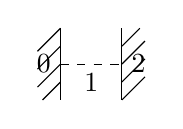
\begin{tikzpicture}[x=0.65cm,y=0.65cm]
\draw (0,-0.7) -- (0,0.7);
\draw (1.2,-0.7) -- (1.2,0.7);
\draw[dashed] (0,0) -- (1.2,0);
\node[left] at (0,0) {$0$};
\node[below] at (0.6,0) {$1$};
\node[right] at (1.2,0) {$2$};
\draw (-0.45,0.25) -- (0,0.7);
\draw (-0.45,-0.1) -- (0,0.35);
\draw (-0.45,-0.45) -- (0,0);
\draw (-0.35,-0.7) -- (0,-0.35);
\draw (1.2,0.35) -- (1.55,0.7);
\draw (1.2,0) -- (1.65,0.45);
\draw (1.2,-0.35) -- (1.65,0.1);
\draw (1.2,-0.7) -- (1.65,-0.25);
\end{tikzpicture}
\end{adjustbox}
\quad $0\leq\operatorname{Re}s\leq2$ --- крит. полоса.

\SourcePage{GELFAND-P001115}{unlabelled}
\underline{5/IX-83 г.}\quad \underline{Сем. Гельфанда.}

\underline{Делинь. Теоремы конечности когомологий для семейств алгебраических многообразий.}

Раб. FALTINGS'a и его вариации.\quad Всё над $\mathbb C$.

$C$ --- алг. кривая (комп. рим. пов.)

$S$ --- конечн. подмн-во в $C$.

\SourceFigure{GELFAND-P001115}{family-arrow}{Слева $A$, под ним зачернённый вертикальный соединительный знак, ниже $C-S$. Наконечник знака неразличим.}
(сем-во алг. мн-гий, параметр. точками $C-S$)

\begin{adjustbox}{max width=\linewidth}
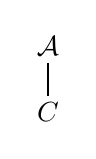
\begin{tikzpicture}[x=0.7cm,y=0.7cm]
\node at (0,1.2) {$\mathcal A$};
\draw (0,0.9) -- (0,0.3);
\node at (0,0) {$C$};
\end{tikzpicture}
\end{adjustbox}
\quad мод. Нерона:
\Unclear{GELFAND-P001115}{neron-overwritten-letter}{$\mathcal A$?}
над $C\setminus S$ абелево мн-гие, а
в $S$ --- расшир. аб. мн-гия
[зачеркнуто: \Unclear{GELFAND-P001115}{neron-cancelled-word}{неразборчиво}]
\Incomplete{GELFAND-P001115}{neron-cancelled-word-loss}{Длинное зачёркнутое слово перед «мультипл. группами» не восстановлено; читаемые окружающие слова сохранены.}
мультипл. группами $\mathbb C^*$.

[Вставлено над описанием модели Нерона: можно сделать так (после конечного накрытия $C$).]

Задача --- продолжить рассл. с $C-S$ на всё $C$.

\begin{equation*}
 A=\operatorname{Lie}A/\Gamma,
 \qquad \Gamma\text{ --- решётка, мен. от слоя к слою}.
\end{equation*}
\begin{equation*}
 A_3=\tfrac13\Gamma/\Gamma\simeq
 \text{\Unclear{GELFAND-P001115}{locally-word}{locally?}}\,.
 (\mathbb Z/3)^{2d},\qquad d=\dim_{\mathbb C}.
\end{equation*}
[Под $A_3$: точки 3-го порядка в $A$.]
[Под латинским словом: локальная система.]

(можно любое число $\geq3$)

Если сист. тривиальна, то можно продолжить $A$ на $S$.
\begin{equation*}
 (\mathbb C^*)^e\longrightarrow\mathcal A\longrightarrow
 \underset{b}{B};\qquad b+e=d.
\end{equation*}
Один период тора увелич. и $\to\infty$
(и [зачеркнуто: \Unclear{GELFAND-P001115}{period-cancelled}{неразборчиво}]
[вставлено: это напр.] превращается в $\mathbb C^*$)
(Нерон).

\begin{adjustbox}{max width=\linewidth}
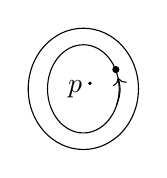
\begin{tikzpicture}[x=0.7cm,y=0.7cm]
\draw (0,0) ellipse (1 and 1.1);
\draw (0,0) ellipse (0.65 and 0.8);
\draw[->] (0.60,-0.30) .. controls (0.68,-0.1) and (0.68,0.02) .. (0.63,0.2);
\fill (0.59,0.35) circle (0.065);
\node at (-0.15,0) {$p$};
\fill (0.12,0.1) circle (0.035);
\end{tikzpicture}
\end{adjustbox}
\quad $T:\Gamma\to\Gamma$ (монодромия) около точки $p\in S$.

Соб. знач. $T$ --- корни из $1$.

$T$ унипотентен $\Longleftrightarrow$ его редукция $\bmod3$ тождественна (единична)
(или любому модулю).
\Unclear{GELFAND-P001115}{unipotent-equivalence}{[Двусторонняя стрелка и приписка о модуле сохранены как в источнике.]}

(\Unclear{GELFAND-P001115}{matrix-initial}{$T$ или $\Gamma$}-матр. с целыми алг. элементами)

[Над следующей формулой: $\operatorname{Lie}/C$.]
\begin{equation*}
 \left(\bigwedge^d\operatorname{Lie}\right)^\vee
 =\omega=\text{line bundle}/C.
\end{equation*}
[Под $\bigwedge^d$: max внешн. степ.]

\underline{Теор.} (Faltings)
\begin{equation*}
 |\operatorname{deg}(\omega)|\leq f(g,|S|)
\end{equation*}
[Перед закрывающей скобкой вставлено сверху: $\dim$.]
(универс. оценка)

(типа $6g+|S|$)

\underline{Пример.}

[Слева, одна над другой, записи: $\Gamma_t$; $t$.]
\begin{equation*}
 \underline{\pi_1(C-S,t)\longrightarrow GL(\Gamma_t)}
\end{equation*}
Это один из немногих способов строить интересные дискр. группы.

\SourcePage{GELFAND-P001116}{76}
\underline{Способ постр. сем-ва аб. мн-гий.}

$C\subset$ [зачеркнут знак: \Unclear{GELFAND-P001116}{ambient-cancelled}{неразборчиво}]
$(\mathbb P^1)^5$
\begin{equation*}
 y^N=\prod(x-x_i)^{m_i}
\end{equation*}
(кривая, завис. от $5$ [вставлено сверху: различных] точек $x_i$)

Надо рассм. якобиан $\longrightarrow$ получим сем-во абелевых мн-гий.

($C$ --- кривая в мн-во пятёрок точек)

$S$ --- пересечение $C$ с мн-вом, где какие-то $x_i$ совпадают.

Так построены в $SU(2,1)$ и $SU(3,1)$ неарифметич. подгруппы\ldots
(\underline{Делинь, Мостов}) [под именами: препринт].

Это связано с \Unclear{GELFAND-P001116}{hypergeometric-abbreviation}{гип.?} ф-й
\begin{equation*}
 \int_{x_1}^{x_2}\prod(X-x_i)^{m_i}\,dX
\end{equation*}
Terada (недавно)

Lauricella (прошлый век)

\underline{2 следствия теор. Faltings'a}

а) Фиксируем $C,S$ и будем рассм. сем-ва, снабж. главной поляризацией
(напр., якобианы)
$\longrightarrow$ представлений, возник. так, возн. лишь конечн. число
(с точн. до изом.)

б) мен. кривую, но фикс. род и число точек. Получ. предст. другой группы.
Всё равно ``конечное число'': \underline{кривые} и \underline{$S$} соединяются гомотопией\ldots

\begin{adjustbox}{max width=\linewidth}
\begin{tikzcd}
 X\subset\mathbb P^N\times(C-S)\arrow[d]\\
 C-S
\end{tikzcd}
\end{adjustbox}
\quad сем-во проект. несингул. мн-гий
(уже \underline{неабелевых}, вообще говоря).

\begin{equation*}
 \pi_1(C-S,t)\longrightarrow GL\bigl(H_i(X_t,\mathbb Z)/\text{Torsion}\bigr).
\end{equation*}
[Обозначение $GL$ вставлено над строкой после стрелки.]

c) $\dim H_i$ ограничена $\Longrightarrow$ получ. конечное число представл.

$\boldsymbol{\longrightarrow}$ структура Ходжа на гомологиях.

\underline{12/IX-83 г.}\quad \underline{Сем. Гельфанда.}

\underline{Арнольд В.И.}

\underline{О конгрессе.}\quad \underline{Сато}: о корреляционных функциях и т.п.

\underline{McPherson}: глоб. вопросы теории сингулярных пространств.

\underline{Докл. Стэнли.}\quad
\underline{Комбинаторные следствия трудной теор. Лефшеца}
(о гиперплоском сечении)

$m,n\in\mathbb Z,\quad m,n>0$.

\begin{adjustbox}{max width=\linewidth}
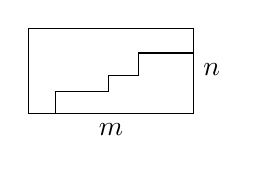
\begin{tikzpicture}[x=0.7cm,y=0.7cm]
\draw (0,0) rectangle (3,1.55);
\draw (0.5,0) -- (0.5,0.4) -- (1.45,0.4) -- (1.45,0.7) -- (2,0.7) -- (2,1.1) -- (3,1.1);
\node[below] at (1.5,0) {$m$};
\node[right] at (3,0.8) {$n$};
\end{tikzpicture}
\end{adjustbox}

Рассм. все диагр. Юнга, умещ. внутри.
Упорядочим все диагр. (частично, по включению).

$L_{m,n}$ --- такое частично упор. мн-во.

$L_{2,3}$
\SourceFigure{GELFAND-P001116}{young-poset-sketch}{Внизу схема диаграмм Юнга: $\varnothing$, одна клетка, вертикальная пара, горизонтальная пара, горизонтальный ряд из трёх, угловая трёхклеточная диаграмма, диаграмма с рядами $3,1$, квадрат $2\times2$, диаграмма с рядами $3,2$, прямоугольник $2\times3$. Видны стрелки от $\varnothing$ к одной клетке, от одной клетки к вертикальной паре, от горизонтальной пары к ряду из трёх; две кривые линии между первыми диаграммами пересекаются, их принадлежность и направления требуют проверки по скану.}

\SourcePage{GELFAND-P001117}{unlabelled}
\underline{Ширина} структуры = макс. число попарно невлож. диаграмм.

\underline{Теор.} Ширина структ. $L_{m,n}$ = числу диаграмм средней мощности
(т.е. мощности $[\tfrac12mn]$).

См. выше; ширина $L_{2,3}$ равна $2$.

(Нет простого комбинаторного док-ва)

\underline{Д-во:} рассм. мн-гие Грассмана $G_{m,m+n}$.
Его гомол. выч. с пом. клеток Шуберта (построенных с пом. репера)

(Флаг; строчки --- размерности пересечений с разными пр-вами флага)

Клетки = гомологии (т.к. все размерности чётные)

Площадь графика = размерность клетки.

Вложение диагр. = включение клеток.

\underline{Мн-гие --- кэлерово} (и даже проективное --- отобр. Плюккера,
частн. случай отобр. Веронезе для торических мн-гий)
\begin{equation*}
 H^i\overset{\wedge\omega^{N-i}}{\longrightarrow}H^{2N-i}
 \qquad\text{Это Изоморфизм (теор. Лефшеца)}
\end{equation*}
(внешнее умн.)

В \underline{гомологиях}: пересеч. с двойственной
[зачеркнуто: \Unclear{GELFAND-P001117}{dual-cell-cancelled}{Шуберта?}]
\Incomplete{GELFAND-P001117}{dual-cell-cancelled-loss}{Зачёркнутое слово не восстановлено полностью; «Шуберта?» сохранено только как кандидат, середина остаётся неразборчивой.}
клеткой.

\underline{И.М.Г.}\ \underline{Хоррокс} (недавно сравн.) --- вычис.
[вставлено: точн.] связь классов Черна (базис) с базисом, получ.
из клеток Шуберта.

\underline{А.}\quad \underline{2-я часть.}
\begin{equation*}
 \alpha_0-\alpha_1+\alpha_2=2\qquad(\text{теор. Эйлера для многогр.})
\end{equation*}
\begin{equation*}
 \alpha_0-\alpha_1+\ldots+(-1)^{d-1}\alpha_{d-1}=1+(-1)^{d-1}.
\end{equation*}
Если все грани симплиц., то
[зачеркнуто: \Unclear{GELFAND-P001117}{simplicial-cancelled}{неразборчиво}]
\Incomplete{GELFAND-P001117}{simplicial-cancelled-loss}{Зачёркнутый фрагмент между «то» и «есть доп. соотношения» не восстановлен; соседний текст сохранён.}
есть доп. соотношения.

\underline{Косимплициальные}
[зачеркнуто: \Unclear{GELFAND-P001117}{cosimplicial-cancelled}{неразборчиво}]:
\Incomplete{GELFAND-P001117}{cosimplicial-cancelled-loss}{Зачёркнутое короткое слово перед двоеточием не восстановлено; окружающая запись сохранена.}
углы все симплициальные (двойств. симплициальным).

\begin{equation*}
 \left.\begin{array}{ll}
 \text{Ден}&\text{Dehn}\\
 \text{Зоммервиль}&\text{Sommerville}\\
 \text{Мак Муллен}&\text{Mac Mullen}
 \end{array}\right\}
\end{equation*}
Стэнли

[Справа от скобки:]
см. статью Арнольд-78 г. \Unclear{GELFAND-P001117}{reference-preposition}{из или у} ФА.
ссылки см. в докл. Стэнли на конгрессе 1983 г.
Mac Mullen --- есть кн. ``Выпуклые многогр.''

\begin{equation*}
 \alpha_0-2\alpha_1+4\alpha_2=8
\end{equation*}
\Unclear{GELFAND-P001117}{cube-cancelled-operator}{[Знак перед $2\alpha_1$ полностью зачёркнут и не восстановлен; $-$ в формуле — только кандидат по математическому контексту.] }
(см. куб, например)

\underline{Опр.}
\begin{equation*}
 p(t)=\alpha_0+(t-1)\alpha_1+(t-1)^2\alpha_2+\ldots
 +(t-1)^{d-1}\alpha_{d-1}+(t-1)^d
\end{equation*}
(мн-н Пуанкаре многогр.)

[Зачеркнуто: Теор.] \underline{Теор. Дэна}:
1) многочлен $p(t)$ возвратен ($\Rightarrow$ тождество).

2) коэфф.
\begin{adjustbox}{max width=\linewidth}
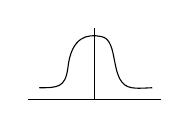
\begin{tikzpicture}[x=0.7cm,y=0.7cm]
\draw (-1.2,0) -- (1.2,0);
\draw (0,0) -- (0,1.3);
\draw (-1,0.22) .. controls (-0.65,0.22) and (-0.53,0.23) .. (-0.48,0.58)
 .. controls (-0.42,1.15) and (-0.12,1.2) .. (0.12,1.15)
 .. controls (0.47,1.1) and (0.25,0.28) .. (0.68,0.22)
 .. controls (0.84,0.2) and (0.95,0.22) .. (1.05,0.22);
\end{tikzpicture}
\end{adjustbox}
(унимодальны --- горкой) (Стэнли)

\underline{Задача}: определить по набору чисел, может ли он служить набором
$\alpha_0,\alpha_1,\alpha_2,\ldots,\alpha_d$.

\underline{Теор.} (Billera, Lee; другое док-во --- Стэнли)
Нек-рое необх. и дост. условие.

\SourcePage{GELFAND-P001118}{77}
$h_j$ --- коэффициенты.
\begin{equation*}
 h_0=1=h_d,\qquad h_{d-i}=h_i\qquad(\text{возвратность})
\end{equation*}
Необх. и дост., чтобы сущ. градуир. алгебра (ассоц., коммут.)
\begin{equation*}
 R=R_0\oplus R_1\oplus\ldots\oplus\ ,
 \qquad\text{порождённая }R_1\text{ над }R_0=\mathbb C,
\end{equation*}
\Unclear{GELFAND-P001118}{graded-sum-ending}{[После последнего $\oplus$ в источнике оставлен пробел.]}
\begin{equation*}
 R_iR_j\subseteq R_{i+j},\qquad R_0=\mathbb C
\end{equation*}
и при этом
\begin{equation*}
 \dim_{\mathbb C}R_i=h_i-h_{i-1},\qquad 0\leq i\leq[d/2].
 \qquad(\text{из т. Лефшеца})
\end{equation*}
($\Rightarrow$ унимодальность, т.к. $h_i\geq0$)
\Unclear{GELFAND-P001118}{unimodality-sign}{[В рукописи именно $h_i\geq0$, без разности соседних коэффициентов.]}

\underline{Д-во}: из теор. Лефшеца.

По многогр. строим мн-гие (алгебраическое).
[Вставлено между строками: торическое $\longrightarrow$ см. Данилов в УМН.]

Двойств. многогр. --- симплициальный.

Сделаем его целочисленным --- аппроксимация + растяжение.

$\Rightarrow$ мн-гие строится.

Алгебра:
\begin{equation*}
 R=H^*(X)/(\omega),\qquad h_i=\dim H^{2i}(X)\qquad(\text{см. Данилов})
\end{equation*}
[Под $(\omega)$: идеал, пор. $\omega$.]

Важно, что симплиц. $\boldsymbol{\Rightarrow}$ получ. кэлерово мн-гие.

[На левом поле: \Unclear{GELFAND-P001118}{margin-middle}{4 или 7?}.]
\begin{equation*}
 \dim R_i=\dim H^{2i}-\dim(\omega H^{2i-2})
 =\dim H^{2i}-\dim H^{2i-2}=
\end{equation*}
[Под равенством: \underline{Лефшец} (ничего не исчезает из средней групп.).]

\underline{Ещё было:}
\begin{equation*}
 \left.\begin{array}{l}
 \text{Thurston}\\
 \text{Yau}\\
 \text{A. Connes}
 \end{array}\right]
 \quad(\text{вне программы})\quad\underline{3\text{ премии Филдса}}.
\end{equation*}

[На левом поле: \Unclear{GELFAND-P001118}{margin-lower}{неясные знаки перед закрывающей скобкой}.]

\underline{Yau} --- есть обзор и есть список нереш. проблем
(Princeton, конф. по геометрии)
[Под строкой: 1--2 года назад.]

Из докл. \underline{Винберга} (по Мостову) видно, что
соотн. эти явл. основой
в теор. Винберга:
в пр-ве Лобачевского разм. $\geq30$ нет групп, порожд. отражениями.

\underline{Thurston.}\quad $z\mapsto z^2+i$

Итерации (вообще рац. ф-и). Есть раб. Милнора, Дуади, Сулливана.
(дин. система и т.д.)

Смотрим образ точки $0$ (критич.).
\begin{equation*}
 0\mapsto i\mapsto-1+i\mapsto-i\mapsto-1+i\mapsto\ .
\end{equation*}
Крит. точка попад. на 2-цикл и там остаётся.

\underline{Гипотеза}: \underline{отобр. с этим св-вом плотны}:
образ крит. точки с нек-рого момента стан. периодической.

Осн. рез. --- с пом. машин.

\underline{Теор.} Рассм. фунд. область на пл. Лобачевского.
\SourceFigure{GELFAND-P001118}{hyperbolic-domain}{Справа внизу окружность с вписанной криволинейной четырёхугольной фигурой; через фигуру и за окружность проходят несколько длинных наклонных петель или штрихов. Подписей нет. На верхней левой внутренней кривой различимы отдельный стержень и наконечник стрелки, направленной вверх и вправо. Различение остальных петель, стрелок, границы области и зачёркивающей штриховки остаётся неопределённым.}

\SourcePage{GELFAND-P001119}{unlabelled}
\begin{adjustbox}{max width=\linewidth}
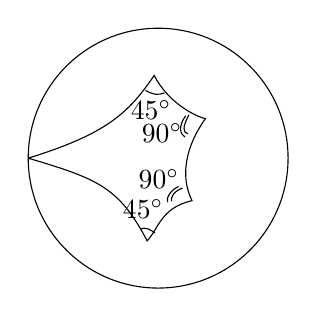
\begin{tikzpicture}[x=1cm,y=1cm]
\draw (0,0) circle (1.65);
\draw (-1.65,0) .. controls (-0.65,0.31) and (-0.38,0.57) .. (-0.05,1.05)
 .. controls (0.12,0.72) and (0.43,0.55) .. (0.6,0.5)
 .. controls (0.36,0.17) and (0.27,-0.22) .. (0.43,-0.54)
 .. controls (0.03,-0.63) and (0.0,-0.91) .. (-0.14,-1.05)
 .. controls (-0.5,-0.36) and (-0.78,-0.26) .. (-1.65,0);
\draw (-0.16,0.86) .. controls (-0.05,0.80) and (0.01,0.8) .. (0.08,0.83);
\draw (0.39,0.55) .. controls (0.31,0.4) and (0.31,0.32) .. (0.38,0.31);
\draw (0.35,0.54) .. controls (0.25,0.4) and (0.28,0.3) .. (0.34,0.27);
\draw (0.31,-0.38) .. controls (0.2,-0.42) and (0.16,-0.49) .. (0.17,-0.55);
\draw (0.26,-0.36) .. controls (0.15,-0.41) and (0.1,-0.51) .. (0.12,-0.56);
\draw (-0.23,-0.9) .. controls (-0.15,-0.87) and (-0.1,-0.91) .. (-0.04,-0.95);
\node at (-0.09,0.61) {$45^{\circ}$};
\node at (0.05,0.32) {$90^{\circ}$};
\node at (0.01,-0.27) {$90^{\circ}$};
\node at (-0.19,-0.65) {$45^{\circ}$};
\end{tikzpicture}
\end{adjustbox}
[На верхней правой дуге внешней окружности видна небольшая стрелка, направленная влево вдоль окружности.]

Отображение:
есть модель с отр. кривизной,

Надо ввести \Unclear{GELFAND-P001119}{metric-abbreviation}{рим.? / рив.?} метрику отриц. кривизны на плоскости
без точек $i,-i,-1+i,0$ и $\infty$
(крит. точку и образы).

Взять универс. накрыв. и там метрику пост. отриц. кривизны.

Обр. отобр. --- растяжение в этой метрике (равномерное).

Полезно --- 2-листное накрытие.

На накрывающей особые точки исчезнут и т.д.

Башня рим. поверхностей и т.д.

\underline{Оконч. результат:}

[Справа:]
Мн-во Жюлиа --- неблуждающие точки, --- универсальное дерево с
\Unclear{GELFAND-P001119}{branching-adjective}{тройным? / кратным?} ветвлением.

Теория есть $\forall$ рац. числа.
\Unclear{GELFAND-P001119}{rational-numbers-word}{[В последней строке написано «числа», не «функции».]}

\SourcePage{GELFAND-P001120}{unlabelled}
\underline{26/IX-83 г.}\quad \underline{Сем. Гельфанда}

\underline{Переломов} (о раб. Witten'a)

препринт --- ``Нуклон как солитон''

\underline{``Алгебра токов, барионы и удержание кварков''}

``Барион --- частица с ненулевым барионным зарядом''

Сохр. зарядов (из анализа превращений):

$Q$ --- эл. заряд

$B$ --- бар. заряд

\Unclear{GELFAND-P001120}{strangeness-symbol}{$\zeta$ или $S$} --- странность

$L$ --- лептонный заряд

\underline{До 1974 г.}\quad Частице --- поле $\Psi(x)$ и действие
\begin{equation*}
 S=[\Psi_1,\ldots,\Psi_N]=\int d^4x\,\mathcal L(\Psi_1,\ldots,\Psi_N).
\end{equation*}
Пишется так, чтобы все заряды сохранялись.

Частицы вх. парами $\Psi(x),\overline\Psi(x)$ (частица и античастица)
[Под $\overline\Psi(x)$: компл. сопр. ф-я.]

$B=1$ $\Rightarrow$ нельзя писать $\int\Psi^2(x)d^4x$;
можно $\int\overline\Psi\Psi\,d^4x$.

(будет матр. элемент, соотв. проц. с рожд. бариона)

$\forall$ Элем. частице $\rightsquigarrow$ поле.
Лагранжиан пишется из общих принципов.
// $\forall$ реакции $\mapsto$ слагаемое в лагранжиане

$\forall$ Взаимодействию тоже отвечает частица.

$\Downarrow$

есть \underline{гравитон}

[Справа:]
\begin{equation*}
 \underbrace{e+\bar e\;\text{ --- фотон}}
 \quad\Longrightarrow\quad\overline\Psi\gamma^\mu\partial_\mu\Psi A
 \qquad\text{и т.д.}
\end{equation*}
\Unclear{GELFAND-P001120}{photon-expression}{[Между $\gamma^\mu$ и $\Psi$ в исходной формуле написано $\partial_\mu$; у $A$ индекс не указан.]}

[Зачеркнуто: \Unclear{GELFAND-P001120}{skyrme-cancelled-date}{неясные цифры}.]
\Incomplete{GELFAND-P001120}{skyrme-cancelled-date-loss}{Отменённая многозначная дата не восстановлена полностью; видимые остатки и незачёркнутая дата 1961 сохранены.}
1961 (Скирм) (не обратили на неё вним.) --- была геом.
[зачеркнуто: \Unclear{GELFAND-P001120}{geometric-cancelled}{неразборчиво}]
\Incomplete{GELFAND-P001120}{geometric-cancelled-loss}{Зачёркнутое короткое слово или сокращение перед «структура» не восстановлено; нижний выносной штрих остаётся видимым остатком.}
структура.

1974 г. 't Hooft, Поляков $\Rightarrow$ геом. напр. стало разв. после них.
[Под 't Hooft: (Тофт).]

Witten тоже относится к геом. направлению.

\SourcePage{GELFAND-P001121}{80}
Модели наз. \underline{киральными} мод. или \underline{$\sigma$-моделями}.

$M^4$ --- пр-во Минковского,
$\varphi\colon M^4=\mathbb R^3\times\mathbb R^1\longrightarrow(\Phi,g)$.
[Под $(\Phi,g)$: риманово мн-гие.]

$\varphi(x)$ --- поле со знач. в рим. мн-гии //

Действие:
\begin{equation*}
 (1)\qquad S=\int(\partial_\mu\varphi,\partial_\mu\varphi)d^4x
 =\int(h_{\alpha\beta}\partial^\alpha\varphi,\partial^\beta\varphi)d^4x;
 \quad\partial_\mu\varphi=\varphi_*\frac{\partial}{\partial x_\mu}.
\end{equation*}
\Unclear{GELFAND-P001121}{action-indices}{[Во втором интеграле индексы $\alpha,\beta$ написаны над $\partial$, не над $\varphi$; у первого коэффициента читается $h$, хотя выше метрика обозначена $g$.]}

Уравнение:
\begin{equation*}
 (2)\qquad\delta S=0
\end{equation*}
или
\begin{equation*}
 (2')\qquad\partial_\mu\partial_\mu\varphi^\alpha
 +\Gamma^\alpha_{\beta\delta}\partial_\mu\varphi^\beta
 \partial_\mu\varphi^\delta=0,
\end{equation*}
откуда это --- обобщение ур-я геодезических.

Требование:
\begin{equation*}
 (3)\qquad\pi_3(\Phi)\ne0
\end{equation*}
\begin{equation*}
 \varphi(x)=\varphi(\bar x,t)
\end{equation*}
При фиксир. $t$ возникает отображение $\mathbb R^3\to\Phi$.
\begin{equation*}
 (4)\quad\text{Требуем:}\quad\exists\lim_{|\bar x|\to\infty}
 \varphi(\bar x,t)=\varphi_0(t)
\end{equation*}
\begin{equation*}
 \mathbb R^3\cup\{\infty\}=S^3.
\end{equation*}
Поля разбиваются на гомот. классы (по отобр. $S^3\to\Phi$)

Потребуем:
\begin{equation*}
 (5)\qquad S\ge\varepsilon\quad\text{на гомот. классе}
\end{equation*}
$\Rightarrow$ в $\forall$ гомот. классе есть решение.

\underline{Примеры.}

(6) $\Phi$ --- простая гр. Ли\quad $\Phi=G$\quad (главное киральное поле)

[Вставлено над ``гр. Ли'': (компактная).]

или

(7) $\Phi$ --- орбита присоед. предст. компакт. гр. Ли
\Unclear{GELFAND-P001121}{orbit-final-symbol}{$G$ (зачеркнуто?) или $\mathfrak g$}.

(8) $\Phi=S^2$ --- $\bar n$-поле

[Справа в рамке: киральное поле $=$ $=$ chirality.]

1954\quad \underline{A. Borel}\quad --- $\forall$ орбита комп. простой гр. Ли --- кэлерова

1954\quad Goto\quad [знаки повтора предыдущей фразы] рациональна

[Ниже: короткая линия, точка и короткая линия.]

2-мерный случай:
\begin{equation*}
 S^2\to\Phi,\quad\Phi=G/H\qquad(G\text{ --- простая компактная})
\end{equation*}
\begin{equation*}
 \pi_2(\Phi)=\pi_1(H)\ne0
\end{equation*}
Перейдём к кэлеровой метрике. Ур-я перех. в ур-я Коши--Римана:

\SourcePage{GELFAND-P001122}{unlabelled}
\begin{equation*}
 (9)\qquad\partial_{\bar z}\varphi=0\qquad(\Leftrightarrow\ \varphi\text{ голоморфно})
\end{equation*}
(т.е. реш. --- голом. отображения)

(Компл. структура: $G/H\sim$ пр-ву флагов; это неск. способами
($|W|$ способов [под $W$: гр. Вейля]))

\underline{Матр.} $=$ (треуг.) $\times$ (унитарную)

$\Phi$ компактно [зачеркнуто:
\Unclear{GELFAND-P001122}{compact-cancelled}{неразборчивый короткий знак}];
неизвестно, есть ли непостоянные решения.

Чтобы было большое число реш.; [зачеркнуто:
\Unclear{GELFAND-P001122}{rational-cancelled}{неразборчиво};
вставлено сверху: (достат., чтобы)] $\Phi$ рационально
(т.е. поле ф-й на $\Phi$ изоморфно полю рац. ф-й нек-рого числа переменных).
\begin{equation*}
 \mathbb CP^1\longrightarrow\Phi\quad(\text{кэлерово мн-гие})
\end{equation*}
$\Rightarrow$ есть большое число инстантонных решений

$\Phi=S^2$ --- Белавин, Поляков. (из стереогр. проекции)

$\Phi=G$ --- простая компактная группа Ли.
\begin{equation*}
 \begin{aligned}
  \pi_1(G)&=0\\
  \pi_2(G)&=0\\
  \pi_3(G)&=\mathbb Z_2
 \end{aligned}
\end{equation*}
\Unclear{GELFAND-P001122}{third-homotopy}{[Перед $\mathbb Z_2$ зачеркнут знак, похожий на $0$; индекс $2$ после $\mathbb Z$ оставлен как в источнике.]}
\begin{equation*}
 \pi_4(SU(3))=0,\quad\pi_4(SU(2))=\mathbb Z_2,\quad\pi_5(SU(2))=\mathbb Z_2.
\end{equation*}
Огранич. снизу нет:

при замене [зачеркнуто:
\Unclear{GELFAND-P001122}{scaling-cancelled}{$\varphi$?}]
$\mathbf x$ на $\lambda\mathbf x$: $S$ на $\lambda^2S$
$\Rightarrow S$ можно сделать сколь угодно малым.

[Сверху к $\lambda\mathbf x$ направлена стрелка с подписью: замена в $M^4$.]

(10) На самом деле $S=S_0+S_1+S_2$
\begin{equation*}
 (11)\qquad S_0=\int\operatorname{tr}
 \bigl(\underbrace{g^{-1}\partial_\mu g}_{A_\mu}\cdot g^{-1}\partial_\mu g\bigr)d^4x
\end{equation*}
для унит. матриц ($SU(3)$ или $SU(2)$)

[Справа:] $A_\mu$ --- эл-т алгебры Ли
\begin{equation*}
 (12)\qquad S_2=\int d^4x\,\operatorname{tr}
 \bigl([A_\mu,A_\nu]\colon[A_\mu,A_\nu]\bigr)
\end{equation*}
\Unclear{GELFAND-P001122}{commutator-separator}{[Между коммутаторами две точки; двоеточие либо точка умножения с помаркой.]}

Произв. по $t$ входят квадратично $\to$ уже инвариантно отн. гомотетии в $M^4$

$S_0+S_2$ уже имеет [зачеркнуто:
\Unclear{GELFAND-P001122}{instanton-cancelled}{соли\ldots?}]
\Incomplete{GELFAND-P001122}{instanton-cancelled-loss}{Полное зачёркнутое слово не восстановлено; «соли\ldots?» сохранено только как фрагмент-кандидат.}
инстантонные решения.

$S_1$ доб., чтобы можно было отличить бозоны от фермионов

Wess, Zumino (1970) добавили $S_1$, но ф-ла сложна

Witten сильно упростил эту ф-лу для $S_1$

Компактифицируем время:
\begin{equation*}
 \begin{aligned}
 M^4=S^3\times S^1&\longrightarrow G=SU(3)\\
 \Vert\qquad&\\
 \partial Q,\quad Q=S^3\times D^2&
 \end{aligned}
\end{equation*}
(13) \underline{Утв.} Отобр. продолжается до непр. отобр. $Q$

(из того, что $\pi_1(G)=0$\quad $\pi_4(G)=0$
[справа от этих двух равенств вертикальная штрихованная скобка].)

[Справа:] Переделываем в отобр.
$S^1\to\operatorname{Map}(S^3,SU(3))$

[Подчеркнуто $\operatorname{Map}(S^3,SU(3))$; ниже: топология этого
\Unclear{GELFAND-P001122}{mapping-space-note}{восстан.?}.]

\SourcePage{GELFAND-P001123}{81}
Получаем:
\begin{equation*}
 \varphi\colon Q\longrightarrow SU(3)
\end{equation*}
\begin{equation*}
 \begin{aligned}
 \varphi^*\colon H^5(SU(3))&\longrightarrow H^5(Q)\\
 \omega&\longmapsto\widetilde\omega
 \end{aligned}
\end{equation*}
[Перед $H^5(Q)$ зачеркнуто:
\Unclear{GELFAND-P001123}{pullback-cancelled}{$0$?}.]

[Справа:] ($\omega$ --- инвар. форма, [зачеркнуто:
\Unclear{GELFAND-P001123}{form-cancelled}{неразборчиво}], явл. образующей в когомологиях)
\Incomplete{GELFAND-P001123}{form-cancelled-loss}{Зачёркнутое слово после «инвар. форма» не восстановлено; нижние петли в начале и конце остаются видимыми остатками.}

или \underline{гармоническая} // (что то же самое)
\begin{equation*}
 (14)\qquad S_1=N\int_Q\widetilde\omega
\end{equation*}
$N$ подбираем, чтобы получ. целое число.

Выбор продолжения [вставлено: $\varphi$] может менять
[зачеркнуто: \Unclear{GELFAND-P001123}{integral-cancelled}{неразборчивый короткий фрагмент}]
$\int$ на [зачеркнуто:
\Unclear{GELFAND-P001123}{multiple-cancelled}{$2\pi$?}; вставлено: (целое)] кратное $2\pi$.

Когомологии $SU(3)$: $(1+t^3)(1+t^5)$

При деформациях [вставлено: (прод. $\varphi$ на)] $Q$ интеграл не меняется
\begin{equation*}
 (15)\qquad\int_Q\widetilde\omega=\int_{\varphi(Q)}\omega
\end{equation*}
[Справа, отделено двумя вертикальными чертами:]
$e^{iS}$ уже не зависит от выбора продолжения
$\Rightarrow$ $\Rightarrow$ квантовая теория хорошо определена

\underline{Zumino} --- $d$-мерный уже случай (препринт) и там появляются вторичные
хар. классы Черна--Сайменса.

1) \underline{Барионный заряд.}
\begin{equation*}
 \pi_3(\Phi)=\mathbb Z\quad\text{и по теор. Гуревича}\quad H^3(\Phi)=\mathbb Z.
\end{equation*}
\underline{Выраж. для барионного заряда:}
\begin{equation*}
 (16)\qquad B=\int d^3x\,B_0=\frac{1}{24\pi^2}
 \int d^3x\,\varepsilon^{ijk}\operatorname{tr}(A_iA_jA_k)
\end{equation*}
(Виттен предлагает назвать это барионным зарядом)

(инвариантная 3-форма, единственная образующая в $H^3(\Phi)$)

2) \underline{Фермион или бозон?}
\begin{equation*}
 \int e^{iS[\varphi]}d\varphi\qquad\text{--- \underline{амплитуда перехода}}
\end{equation*}
Пусть неподвижен $\Rightarrow$ интеграл равен $e^{-iMT}$,
$M$ --- масса, $T$ --- время

\underline{3/X-84 г.}\qquad\underline{Сем. Гельфанда}

\Unclear{GELFAND-P001123}{talk-date}{[На скане написано 3/X-84 г.; дата не заменена каталожной.]}

\underline{Ю. Л. Далецкий}\qquad\underline{Об обобщении ур-я Власова}

(вместе с Р. Н. Кадобянским)

$g$ --- алг. Ли, $g'$ --- дуальн. пр-во, $\langle\ \rangle$ --- двойств.
\begin{equation*}
 \{f,g\}(\nu)=\langle[f'(\nu),g'(\nu)],\nu\rangle
 \qquad(f,g\text{ --- ф-и на }g')
\end{equation*}
\Unclear{GELFAND-P001123}{dual-variable}{[Буква аргумента во всех следующих формулах: $\nu$ или $v$; здесь передана как $\nu$.]}

$H(\nu)$ --- ф-я на $g'$
\begin{equation*}
 \frac{\partial u}{\partial t}=\{u(\nu),H(\nu)\}
\end{equation*}
\begin{equation*}
 (*)\qquad\frac{d\nu}{dt}+[\operatorname{ad}^*H'(\nu)]\nu=0
 \qquad(\text{сопр. ур-е})
\end{equation*}
\Unclear{GELFAND-P001123}{final-operator}{[Знак в последней строке густо обведён; под крестообразными штрихами виден отдельный нижний горизонтальный штрих. $+$ в формуле оставлен условным кандидатом; возможны $+$, $\pm$ или плюс поверх прежнего минуса. История переправления не установлена.]}
\SourcePage{GELFAND-P001124}{unlabelled}
% Visual review: original 2408 x 3448 frame; full-frame inspection and crops.
% Crop coordinates are original pixels [x0,y0,x1,y1]; scale is nearest-neighbour enlargement.
% Enlargement adds no source detail. OCR was not used.
% Review top: [330,20,2160,1170], 1x.
% Review middle: [300,1120,2280,2220], 1x.
% Review bottom: [240,2190,2300,3290], 1x.
% Review top-first: [360,25,2040,245], 3x.
% Review dynamics-note: [845,905,1870,1140], 3x.
% Review cancellations: [340,1110,2170,1590], 3x.
% Review cited-names: [500,2800,1970,2905], 3x.
% Review integral-cancellation: [840,2910,1110,3080], 6x.
% Review point-mass: [770,765,1060,965], 8x.
$\mathfrak g$ — алг. Ли ф-й $\varphi(x)$, $x\in X$ (на симпл. \Unclear{GELFAND-P001124}{manifold-abbreviation}{мн-ии?}).

Двойств. пр-во — меры $\nu(dx)$.

$h_1(x)$ — энергия част.

$h_2(x_1,x_2)$ — \textquotedblright\ — взаимодействия.
\begin{equation*}
H(\nu)=\int_X h_1(x)\nu(dx)+\frac12\int_X\int_X h_2(x,x')\nu(dx)\nu(dx').
\end{equation*}
\begin{equation*}
X^n\qquad y=(x_1,\ldots,x_n)
\end{equation*}
\underline{Утв.} $\displaystyle\nu=\sum_{k=1}^{n}\nu_{x_k(t)}$ явл. решением ур-я (Климонтович).

[Под $x_k(t)$ скобка и выносная запись:] есть ур-е дв-ния — \underline{\Unclear{GELFAND-P001124}{dynamics-note}{согл. ур. кл. механики?}}.

[Слева зачёркнуто: \Unclear{GELFAND-P001124}{derivative-cancellation}{Ур-е?}.]
\begin{equation*}
H'(\nu)=h_1(x)+\int h_2(x,x')\nu(dx').
\end{equation*}
Получ. поток на пр-ве обобщ. ф-й.

Обобщ. ф-и (меры), сосредот. на конечном числе точек.
Оказывается, что [зачёркнуто: \Unclear{GELFAND-P001124}{paragraph-cancellation-one}{неразборчиво}] ф-и, сосред. на $n$ точках,
[зачёркнуто: \Unclear{GELFAND-P001124}{paragraph-cancellation-two}{неразборчиво}] инвариантны отн. потока. Это эквив. ур-ю Власова.
\begin{equation*}
\nu(dx)=C(q,p)\,dp\,dq
\end{equation*}
\begin{equation*}
\frac{\partial C}{\partial t}+\frac{p}{m}\frac{\partial C}{\partial q}
=\frac{\partial C}{\partial p}\left(V'(q)+\int\frac{\partial\Phi(q,q')}{\partial q}C(q',p')\,dq'\,dp'\right).
\end{equation*}
(Ур-е Власова — бесстолкновительная плазма).
\begin{equation*}
h_1(x)=\frac{p^2}{2m}+V(q);\qquad h_2(x,x')=\Phi(q,q').
\end{equation*}
Всё это верно для супералгебр Ли (см. ур-я Березина — Маринова).

\underline{А. Бейлинсон.}\quad \underline{Об одной раб. Witten'а.}

\underline{Не сущ. калибровочной $SU(2)$-теории с нечётным числом фермионов}

Причина: $\pi_4(SU(2))=\mathbb Z/2\mathbb Z$.

(Раньше физики рассматривали [вставлено сверху: именно] чётное число фермионов).
\begin{equation*}
L=\int d^4x\left(\operatorname{Tr}F_{\mu\nu}^{2}+\bar\psi iD\psi\right)
\end{equation*}
Есть раб. \underline{\Unclear{GELFAND-P001124}{cited-name}{Вигман?} Павел (Борисович)} и Поляков (новая) по этому поводу.
\begin{equation*}
\int d\psi\,d\bar\psi\,dA\,\exp(-L)
\end{equation*}
[Между $\exp$ и $(-L)$ зачёркнуто: \Unclear{GELFAND-P001124}{integral-cancellation}{неразборчивый знак}.]
\begin{equation*}
\pi_4(SU(2))=\pi_0\left(SU(2)^{S^4}\right).
\end{equation*}

\SourcePage{GELFAND-P001125}{82}
% Visual review: original 2408 x 3448 frame; full-frame inspection and crops.
% Crop coordinates are original pixels [x0,y0,x1,y1]; scale is nearest-neighbour enlargement.
% Enlargement adds no source detail. OCR was not used.
% Review upper: [55,10,2350,890], 1x.
% Review lower: [130,815,2350,1960], 1x.
% Review determinant-power: [275,805,1120,1090], 3x.
% Review sign-cancellation: [1660,1185,2060,1320], 6x.
% Review bottom-example: [170,1820,1740,1950], 3x.
% Review whitehead: [125,575,715,743], 3x.
% Review sign-cancellation-check: [1830,1135,2040,1220], 6x.
\underline{Фукс:}

\underline{Надстройка:}\quad $\pi_3(S^2)\longrightarrow\pi_4(S^3)$ — эпиморфизм с ядром $2\mathbb Z$.

\underline{И.М.Г.}\quad \underline{Donaldson:} на $\mathbb R^4$ есть \underline{гладкие структуры, завис. от параметра и}
разные при разных \underline{значениях} параметра!!

Фукс:
\begin{equation*}
0\longrightarrow\mathbb Z\longrightarrow\pi_{4n-1}(S^{2n})
\overset{\text{эпи}}{\longrightarrow}\pi_{4n}(S^{2n+1})\longrightarrow0
\end{equation*}
[Под $\pi_{4n-1}(S^{2n})$:] $\mathbb Z\oplus\text{конечная}$.

[От $\mathbb Z$ выносная линия к записи:] порожд. квадратом Уайтхеда.

\underline{Б.}\quad \underline{Теорема (Witten).}

$\int d\psi$ интерпрет. как $(\det D)^{-1/2}\exp(\ldots)$.
\Unclear{GELFAND-P001125}{determinant-power}{Показатель $-1/2$ в рукописи.}

($A$ фиксир.)

\begin{center}
\begin{adjustbox}{max width=\linewidth}
\begin{tikzpicture}
\draw (0,0) .. controls (0.28,0.6) and (0.28,1.25) .. (0.10,1.65);
\draw (1.55,0) .. controls (1.22,0.5) and (1.29,1.35) .. (1.65,1.7);
\draw[->] (0.20,0.86) .. controls (0.33,1.04) and (0.40,0.77) .. (0.55,0.89)
 .. controls (0.70,1.01) and (0.79,0.77) .. (0.93,0.89)
 .. controls (1.09,1.03) and (1.16,0.83) .. (1.35,0.88);
\node at (0.8,-0.25) {2 половинки орбиты.};
\end{tikzpicture}
\end{adjustbox}
\end{center}
$\sqrt{\det D}$ сменит знак, т.к. нек-рые [зачёркнуто: \Unclear{GELFAND-P001125}{sign-cancellation}{неразборчиво}] соб. знач.
сменят знак при переходе через $0$ $\rightsquigarrow$

$\rightsquigarrow$ надо счит. $0$-е моды опер. Дирака на $S^4\times S^1$.

Соб. знач. делятся на пары [под словом «пары»: $(\lambda,-\lambda)$];
$\sqrt{\det}$ изменит знак при переходе через $0$-ю моду.

Дальше использ. теор. Атьи — Зингера. Она даёт число $0$-х мод $\bmod 2$.

\underline{И.М.Г.}\quad \underline{Общая задача для математиков:}

сделать с помощью операторов то, что делается с пом. фейнман. интегралов.

\underline{Пример.} $\sigma$-модель \Unclear{GELFAND-P001125}{sigma-example-word}{простая?} (см. прежний докл. Переломова) $\longrightarrow$ написать оператор.

\SourcePage{GELFAND-P001126}{unlabelled}
% Visual review: original 2408 x 3448 frame; full-frame inspection and crops.
% Crop coordinates are original pixels [x0,y0,x1,y1]; scale is nearest-neighbour enlargement.
% Enlargement adds no source detail. OCR was not used.
% Review upper: [110,860,2200,1810], 1x.
% Review lower: [115,1780,2390,3280], 1x.
% Review action-cancellation: [240,1095,625,1295], 3x.
% Review orbit-cancellation: [1115,2340,1515,2455], 3x.
% Review pauli-commutator: [400,2755,1570,3080], 3x.
\underline{17.10.83 г.}\qquad \underline{Сем. Гельфанда.}

\underline{А. Бейлинсон.}\qquad \underline{О раб. Witten'а}

[Перед $S$ зачёркнуто: \Unclear{GELFAND-P001126}{action-cancellation}{неразборчивый знак}.]
\begin{equation*}
(1)\qquad S=\int(F,F)+i(\psi,D\psi),\qquad F\text{ — кривизна связности }A
\end{equation*}
[От $S$ выносная запись вниз: действие.]
\begin{equation*}
D:\Gamma(E\otimes S)\longrightarrow\Gamma(E\otimes\bar S)\quad\text{— опер. Дирака}
\end{equation*}
$S$ — канонич. спинорное расслоение на 4-мерном мн-зии.

[Под строкой о $S$:] (2-мерное)

$\psi$ — 2-компон. спинор.

$e^{iS}$ — ф-я на пр-ве пар $(A,\psi)$, калибровочно инвариантная
\begin{equation*}
(2)\qquad\int e^{iS}\,d(A,\psi)\;\text{— ?}
\end{equation*}
\underline{Утв.}\quad $(2)=0$, если число компонент $\psi$ нечётно.

Рассм.
\begin{equation*}
(3)\qquad\int\left(\int e^{-S}\,d\psi\right)dA\qquad\text{(интеграл по мн-зию орбит)}
\end{equation*}
Каждая орбита распад. на 2 куска. [Зачёркнуто: \Unclear{GELFAND-P001126}{orbit-cancellation}{неразборчиво}.]
При любом ест. способе опред. ф-я прин. значения противопол. знака на этих компонентах!
$\Rightarrow$ \underline{отсюда} $(2)=0$.
\begin{equation*}
(4)\qquad\int e^{-S}\,d\psi=\sqrt{\det D}\quad\text{— функция от }A_i
\end{equation*}
\begin{equation*}
(5)\qquad D=\sum\sigma^i\left(\frac{\partial}{\partial x_i}+A_i\right),
\qquad\sigma^i\text{ — матрицы 2-го порядка (Паули)}
\end{equation*}
\begin{equation*}
[\sigma_1,\sigma_2]=i\sigma_3=\begin{pmatrix}i&0\\0&-i\end{pmatrix}
\end{equation*}
\Unclear{GELFAND-P001126}{pauli-factor}{В рукописи $[\sigma_1,\sigma_2]=i\sigma_3$.}
\begin{equation*}
(6)\qquad\pi_0\left(SU(2)^{S^4}\right)=\pi_4(SU(2))=\pi_4(S^3)=\mathbb Z_2
\end{equation*}

\SourcePage{GELFAND-P001127}{84}
% Visual review: original 2408 x 3448 frame; full-frame inspection and crops.
% Crop coordinates are original pixels [x0,y0,x1,y1]; scale is nearest-neighbour enlargement.
% Enlargement adds no source detail. OCR was not used.
% Review top: [110,10,2340,735], 1x.
% Review upper-middle: [85,715,2350,1700], 1x.
% Review lower-middle: [150,1670,2330,2670], 1x.
% Review bottom: [50,2600,2310,3310], 1x.
% Review gamma-symbol: [400,807,900,965], 5x.
% Review interval-close: [1180,1220,1530,1400], 6x.
% Review evolution-cancellation: [455,1705,660,1840], 6x.
% Review operator-insertion: [220,2960,940,3110], 3x.
% Review eigenvalue-sign: [1360,491,1500,615], 6x.
% Review operator-grouping-check: [400,807,1140,965], 5x.
Рассм. $S^4\times S^1$ и на нём рассл. $E$ со связностью.

Деформируем связность [подписано снизу: $A$] в другую [подписано снизу: $A'$] так, чтобы $A$ и $A'$ были связаны
преобр. из 2-й компон. калибр. группы.

(Связности — афф. пр-во)

Тогда $\sqrt{\det D}$ изменит знак!

$\sqrt{\det D}$ учит. половину соб. значений.

[Справа, перед следующей записью, знак: \Unclear{GELFAND-P001127}{eigenvalue-sign}{звёздочка или зачёркнутая буква}.]
Соб. знач. — парами $(\lambda,-\lambda)$.

Нечётное число соб. знач. становится отриц. из полож. и наоборот.

Ур-е Дирака
\begin{equation*}
(7)\qquad\sum\gamma^i\frac{\partial}{\partial x_i}+A_i(x_0,\ldots,x_3,t)
\end{equation*}
\Unclear{GELFAND-P001127}{operator-grouping}{Группировка слагаемых — как в рукописи.}

(По $S^4$ то же самое, что было раньше)

$t$ — параметр деформ. связности; пусть в начале то же, что в конце (калибр. эквивал.)

Рассл. на $S^4\times S^1$ тривиально на $S^4\times[0,1)$ \Unclear{GELFAND-P001127}{interval-close}{Правая скобка: $)$ или $]$?}
и дальше склейка с пом. выбр. элемента калибр. группы $\Rightarrow$ оно станет нетривиальным.
\begin{equation*}
(8)\qquad\left(\sum\gamma^i\frac{\partial}{\partial x_i}+A_i(x_0,\ldots,x_3,t)\right)\psi=0
\end{equation*}
рассм. как эволюционное ур-е

[В начале формулы (9) зачёркнуто: \Unclear{GELFAND-P001127}{evolution-cancellation}{неразборчивые знаки}.]
\begin{equation*}
(9)\qquad\frac{\partial}{\partial t}\psi=B\psi,\quad
\text{где }B\simeq\text{ опер. Дирака на 4-мерном мн-зии.}
\end{equation*}
[Под $B$:] зав. от пар. $t$

Пусть $B$ не зависит от $t$, а вместо отрезка — прямая.

Выберем в качестве $\psi$ соб. ф-ю с соб. знач. $\lambda>0$.
\begin{equation*}
\begin{aligned}
t\longrightarrow-\infty&\quad\Rightarrow\quad\text{ф-я}\longrightarrow0.\\
t\longrightarrow+\infty&\quad\Rightarrow\quad\text{ф-я растёт}
\end{aligned}
\end{equation*}
Хорошо бы убывало при $t\longrightarrow\pm\infty$.

Надо: \underline{чтобы соб. знач. меняло знак.}

Реш. с такими гран. условиями $\approx$ ф-я на окружности.

$\Rightarrow$ по меняющему знак соб. значению строится реш. ур-я Дирака.

Итак, \underline{колич. решений} (8) на $S^4\times S^1$ \underline{связано с переменами знака}
\underline{соб. значений оператора} (7).

Witten говорит «\underline{будем менять адиабатически}» (чтобы всё время была соб. ф-я)

\underline{Теор. А-З.} считает $\bmod 2$ число решений ур-я (8) на $S^4\times S^1$.

Опер. [зачёркнуто: \Unclear{GELFAND-P001127}{operator-cancellation}{неразборчиво}; вписано сверху: \underline{косоэрмитов} $\Rightarrow$],
[зачёркнуто: \Unclear{GELFAND-P001127}{before-count-cancellation}{неразборчиво}] число реш. $\bmod 2$ — топ. инвариант.

И.М.Г. \underline{Задача.} Придумать общую матем. схему, в к-рую это входит как частный случай.

\SourcePage{GELFAND-P001128}{unlabelled}
% Visual review: original 2408 x 3448 frame; full-frame inspection and crops.
% Crop coordinates are original pixels [x0,y0,x1,y1]; scale is nearest-neighbour enlargement.
% Enlargement adds no source detail. OCR was not used.
% Review top: [90,0,2350,1150], 1x.
% Review middle: [95,1110,2340,2110], 1x.
% Review bottom: [80,2020,2330,3300], 1x.
% Review coefficient-symbols: [305,1660,730,1990], 6x.
% Review finite-sequence-note: [415,1010,1270,1130], 3x.
% Review monomial-text: [970,1160,1585,1280], 3x.
% Review coefficient-symbols-check: [305,1660,1460,1990], 6x.
\underline{А. Зелевинский.}
\begin{equation*}
\Lambda_n=\mathbb Z[x_1,\ldots,x_n]^{S_n}\quad\text{— симметрические многочлены}
\end{equation*}
$\Lambda_n^k$ — однородные [вставлено сверху: симм.] многочлены степ. $k$.

$n\longrightarrow\infty\quad\Rightarrow\quad\Lambda_n^k$ перестаёт зависеть от $n$.

[Слева:] Считаем: $n\geq k$.

$\Lambda$ — симм. мно. от «беск.» числа переменных (формализуется — проект. предел)
\begin{equation*}
\begin{aligned}
\text{1-й степ.}\quad&x_1+x_2+\ldots=m_{(1)}\\
\text{2-й степ.}\quad&\left[\begin{aligned}
&x_1^2+x_2^2+\ldots=m_{(2)}\\
&x_1x_2+x_1x_3+x_2x_3+\ldots=m_{(1^2)}
\end{aligned}\right.
\end{aligned}
\end{equation*}
\begin{equation*}
(1)\qquad\lambda=(\lambda_1\geq\lambda_2\geq\ldots\geq\lambda_n\geq\ldots\geq0)
\end{equation*}
(обрывающаяся где-то беск. послд.)
\begin{equation*}
(2)\qquad m_\lambda=x_1^{\lambda_1}x_2^{\lambda_2}\ldots
+\text{ одном., получ. перест. букв.}
\end{equation*}
[Под $x_1^{\lambda_1}x_2^{\lambda_2}\ldots$ — прямая скобка с короткими вертикальными концами.]

Любой — целочисл. лин. комб., так что \underline{$m_\lambda$ — базис}.

(мономиальный базис)
\begin{equation*}
m_{(3\,1^2)}=x_1^3x_2x_3+\ldots
\end{equation*}
[Под многоточием — прямая скобка и подпись: перест.]
\begin{equation*}
\begin{aligned}
p_1&=-m_{(1)}\\
p_2&=m_{(1^2)}\\
p_3&=-m_{(1^3)}\\
&\ldots
\end{aligned}
\qquad x^n+p_1x^{n-1}+p_2x^{n-2}+\ldots=0
\end{equation*}
\Unclear{GELFAND-P001128}{coefficient-symbols}{Буквы коэффициентов: $p_i$, $\rho_i$ или $\beta_i$?}

[Обведено с трёх сторон:] $e_n=m_{(1^n)}$.
\begin{equation*}
(3)\qquad E(t)=\sum_{n\geq0}e_nt^n=\prod_i(1+tx_i)\qquad\text{(производ. ф-я)},\quad e_0=1,
\end{equation*}
\begin{equation*}
\begin{aligned}
(4)\qquad h_n&=\sum_{|\lambda|=n}m_\lambda,\\
h_2&=m_{(2)}+m_{(1^2)}=(x_1^2+x_2^2+\ldots)+(x_1x_2+x_1x_3+\ldots)
\end{aligned}
\end{equation*}
(сумма всех одночленов)
\begin{equation*}
(5)\qquad H(t)=\sum_{n\geq0}h_nt^n=\prod_i(1-tx_i)^{-1}\qquad\text{(Упражнение!)},\quad h_0=1
\end{equation*}
\begin{equation*}
(6)\qquad p_n=m_{(n)}\quad\text{— степенная сумма}
\end{equation*}
\begin{equation*}
(7)\qquad P(t)=\sum_{n\geq1}p_nt^n=\sum_i\frac{tx_i}{1-tx_i}=tH'(t)/H(t)
\end{equation*}
\underline{Базисы:}\quad по $\lambda=(\lambda_1,\lambda_2,\ldots)$ строим:

\SourcePage{GELFAND-P001129}{85}
% Visual review: original 2408 x 3448 frame; full-frame inspection and crops.
% Crop coordinates are original pixels [x0,y0,x1,y1]; scale is nearest-neighbour enlargement.
% Enlargement adds no source detail. OCR was not used.
% Review top: [115,10,2350,980], 1x.
% Review middle: [140,945,2370,2330], 1x.
% Review bottom: [150,2270,2390,3430], 1x.
% Review young-diagram: [390,2820,865,3070], 4x.
% Review tableau-bottom: [970,3140,2360,3420], 3x.
% Review transition-word: [270,1860,525,1990], 3x.
% Review basis-cancellation: [1365,2100,1660,2195], 5x.
% Review theorem-sign: [322,2480,420,2605], 6x.
% Review kostka-positive: [1270,2690,1540,2815], 6x.
% Review column-arrow: [1710,3110,2340,3230], 3x.
\begin{equation*}
(8)\quad\left[\begin{aligned}
e_\lambda&=\prod e_{\lambda_i}&(e_\lambda)&\text{ — $\mathbb Z$-базис в $\Lambda$}\\
h_\lambda&=\prod h_{\lambda_i}&(h_\lambda)&\text{ — $\mathbb Z$-базис в $\Lambda$}\\
p_\lambda&=\prod p_{\lambda_i}&(p_\lambda)&\text{ — $\mathbb Q$-базис в $\Lambda$}
\end{aligned}\right.
\end{equation*}
[На левом поле у второй строки: и.]
\begin{equation*}
\Lambda=\mathbb Z[e_1,e_2,\ldots]=\mathbb Z[h_1,h_2,\ldots]\qquad
\text{(осн. теор. о симметр. мн-нах)}
\end{equation*}
\begin{equation*}
\Lambda_{\mathbb Q}=\mathbb Q[p_1,p_2,\ldots]
\end{equation*}
\begin{equation*}
p_{(2,1^2)}=(x_1^2+x_2^2+\ldots)(x_1+x_2+\ldots)^2
\end{equation*}
\underline{5-й базис.}\quad $S$-функции Шура (появились у Якоби)
\begin{equation*}
\alpha=(\alpha_1,\ldots,\alpha_n)
\end{equation*}
\begin{equation*}
a_\alpha(x_1,\ldots,x_n)=\det(x_i^{\alpha_j})=
\begin{vmatrix}
x_1^{\alpha_1}&x_1^{\alpha_2}&\ldots&x_1^{\alpha_n}\\
x_2^{\alpha_1}&x_2^{\alpha_2}&\ldots&x_2^{\alpha_n}\\
\ldots&\ldots&\ldots&\ldots
\end{vmatrix}
\end{equation*}
[Под определителем:] кососимм. ф-я от $x_1,\ldots,x_n$.
\begin{equation*}
a_\delta=\prod_{i<j}(x_i-x_j)
\end{equation*}
\begin{equation*}
(\delta=(n-1,n-2,\ldots,1,0))
\end{equation*}
$\dfrac{a_\alpha}{a_\delta}$ — симм. многочлен.

Считаем $\alpha_1>\alpha_2>\ldots>\alpha_n$ (с точн. до знака всегда добив.)

\Unclear{GELFAND-P001129}{transition-word}{Иначе:?}
\begin{equation*}
\alpha=\lambda+\delta,\qquad\lambda_1\geq\lambda_2\geq\ldots\geq\lambda_n
\end{equation*}
\begin{equation*}
(9)\qquad s_\lambda\overset{\mathrm{def}}{=}a_{\lambda+\delta}/a_\delta
\quad\text{— ещё один базис.}
\end{equation*}
[Зачёркнуто: \Unclear{GELFAND-P001129}{basis-cancellation}{в … [остальное неразборчиво]}.] (Над $\mathbb Z$)

При $n\geq|\lambda|$ отношение не зависит от $n$.

\underline{Теория:} нах. связи между ними и структурные константы (при умножении)

\underline{Пример — Теорема.}

[Перед формулой зачёркнуто: \Unclear{GELFAND-P001129}{theorem-sign}{неразборчивые знаки}.]
\begin{equation*}
s_\lambda=\sum_\mu K_{\lambda\mu}m_\mu
\end{equation*}
[Под $K_{\lambda\mu}$ — прямая скобка и подпись: числа Костки.]
\begin{equation*}
K_{\lambda\mu}\in\mathbb Z,\qquad K_{\lambda\mu}>0
\end{equation*}
\Unclear{GELFAND-P001129}{kostka-positive}{Строгое $K_{\lambda\mu}>0$ — как в рукописи.}

\SourceFigure{GELFAND-P001129}{young-diagram}{Трёхрядная диаграмма Юнга; справа $\lambda_1$, $\lambda_2$, $\lambda_3$. Число клеток и незамкнутые линии требуют сверки с оригиналом.}

$\lambda$ \underline{задаёт диагр. Юнга}.

$\mu$ — $\mu_1$ единиц, $\mu_2$ двоек, $\ldots$.

[Две вертикальные разделительные черты.]

Заполняем эту диагр. Вдоль строк $\leq$ (неуб.).
По столбцам $\uparrow$ (строго возраст.).

Наз. это \underline{таблицей Юнга}.

[Пример заполнения; слева вертикальная черта:]
\begin{equation*}
\begin{array}{|lll}
1&1&2\\
3&4&\\
5&&
\end{array}
\end{equation*}
[Справа две вертикальные разделительные черты.]

\underline{Число таблиц Юнга} размера $\lambda$ и веса $\mu$ равно $K_{\lambda\mu}$.

\SourcePage{GELFAND-P001130}{unlabelled}
% Visual review: original 2408 x 3448 frame; full-frame inspection and crops.
% Crop coordinates are original pixels [x0,y0,x1,y1]; scale is nearest-neighbour enlargement.
% Enlargement adds no source detail. OCR was not used.
% Review top: [150,30,2310,1220], 1x.
% Review middle: [140,1190,2320,2270], 1x.
% Review bottom: [135,2220,2350,3360], 1x.
% Review psi-power: [310,955,640,1100], 5x.
% Review derivative-index: [460,1285,620,1430], 8x.
% Review monic-cancellation: [1430,1600,1565,1690], 6x.
% Review equivalence-word: [345,2400,730,2510], 3x.
% Review series-letter: [480,3140,690,3290], 6x.
% Review talk-heading: [215,420,1090,525], 3x.
% Review commutator-order-check: [430,2240,1010,2410], 3x.
\underline{Легкое упр.}: найти матр. перехода между другими.

6-й базис $f_\lambda$ (от слова forgotten)

\underline{24/X-83 г.}\qquad \underline{Сем. Гельфанда.}

\underline{И.М. Гельфанд} с раб. \underline{Flashka}
\begin{equation}
L_n=\sum_{s=0}^{n}u_s\frac{\partial^s}{\partial x_1^s},\qquad u_n=1.
\tag{1}
\end{equation}
\begin{equation}
L_n\tilde\psi=k^n\tilde\psi.
\tag{2}
\end{equation}
Рассм. асимпт. реш. при $k\to\infty$
\begin{equation}
\tilde\psi^n=e^{kx}\sum_{0}^{\infty}c_j k^{-j},\qquad c_0=1.
\tag{3}
\end{equation}
\Unclear{GELFAND-P001130}{psi-power}{Над $\tilde\psi$ в (3) стоит $n$.}

\underline{Упр.}: написать рекурр. ф-лы для опред. $c_j$.
\begin{equation}
\chi=\tilde\psi_{x_i}\tilde\psi^{-1}=k+\sum_{1}^{\infty}\chi_j k^{-j}.
\tag{4}
\end{equation}
\Unclear{GELFAND-P001130}{derivative-index}{В (4) индекс читается $x_i$, не заменён на $x_1$.}

Здесь $\chi_j$ не зависит от выбора $\tilde\psi$

$\forall$ целого $m$, $\exists$ опер. $L_m$ порядка $m$ ([зачёркнуто: \Unclear{GELFAND-P001130}{monic-cancellation}{неразборчиво}] со старшим коэфф. 1)
\begin{equation}
(L_m\tilde\psi)\tilde\psi^{-1}=k^m+\varepsilon_m k^{-1}+\ldots
\tag{5}
\end{equation}
Здесь:
\begin{equation*}
L_m=[(L_n)^{m/n}]\quad (\text{Гельфанд — Дикий})\quad =[(L_n)^{m/n}]_+
\end{equation*}
(5) определяет оператор $L_m$ однозначно

Введём переменные $x_2,x_3,\ldots$ так, что
\begin{equation}
\frac{\partial L_n}{\partial x_m}=[L_n,L_m]
\tag{6}
\end{equation}
\Unclear{GELFAND-P001130}{commutator-order}{Порядок в (6): $[L_n,L_m]$.}

или \Unclear{GELFAND-P001130}{equivalence-word}{равносил.?}
\begin{equation}
\frac{\partial\psi}{\partial x_m}=L_m\psi
\tag{7}
\end{equation}
где
\begin{equation}
\psi=e^{\sum_{2}^{\infty}x_j k^j}\tilde\psi.
\tag{8}
\end{equation}
Считаем, что $u_j$ — ф-и от перем. $x_2,x_3,\ldots$
\begin{equation}
\text{Положим}\quad\varepsilon(k)=-1+\sum_{m=1}^{\infty}\varepsilon_m k^{-m-1}
\tag{9}
\end{equation}
\begin{equation}
\Lambda(k)=\sum_{0}^{\infty}k^{-m-1}L_m
\tag{10}
\end{equation}
[Справа:] (Чередник, ФА, 1978)

\SourcePage{GELFAND-P001131}{86}
% Visual review: original 2408 x 3448 frame; full-frame inspection and crops.
% Crop coordinates are original pixels [x0,y0,x1,y1]; scale is nearest-neighbour enlargement.
% Enlargement adds no source detail. OCR was not used.
% Review top: [100,20,2345,1060], 1x.
% Review middle: [110,1030,2380,1950], 1x.
% Review bottom: [130,1880,2395,3360], 1x.
% Review equation-thirteen-index: [800,537,1020,658], 6x.
% Review cancelled-number: [150,845,325,947], 6x.
% Review differential-note: [1550,928,1880,1060], 6x.
% Review tau-exponent: [790,1290,1450,1455], 5x.
% Review fock-attribution: [1370,1900,1705,2070], 3x.
% Review embedding-subscript: [590,2390,735,2505], 8x.
% Review theorem-reference: [180,35,1410,175], 3x.
% Review epsilon-twelve: [1760,405,2045,535], 6x.
% Review representation-heading: [205,1740,905,1840], 3x.
% Review derivative-scope-check: [790,335,1580,525], 3x.
% Review tau-potential-check: [435,1080,1210,1290], 3x.
Теор. Чередника 3.1 утв., что.
\begin{equation}
\left(\frac{\partial}{\partial x_1}-\chi(k)\right)\Lambda(k)=\varepsilon(k)
\tag{11}
\end{equation}
\underline{Чередник:}
\begin{equation}
\sum_{m=0}^{\infty}k^{-m-1}
\left(\frac{\partial}{\partial x_1}(L_m\psi(k))\psi^{-1}(k)\right)
=\frac{\partial\chi}{\partial k}+\mathcal E(k).
\tag{12}
\end{equation}
\Unclear{GELFAND-P001131}{derivative-scope}{Скобки и область действия производной в (12) — как написано.}
\Unclear{GELFAND-P001131}{epsilon-twelve}{Последний знак в (12): $\mathcal E(k)$ или $\varepsilon(k)$?}
\begin{equation}
-\ell\chi_\ell+\varepsilon_\ell=\frac{\partial}{\partial x^{i}}(\ldots)
\tag{13}
\end{equation}
\Unclear{GELFAND-P001131}{equation-thirteen-index}{В знаменателе (13): $x^i$, $x_i$ или $x_1$?}
\begin{equation}
\begin{aligned}
\frac{\partial}{\partial x_1}(L_m\psi(k)\psi^{-1}(k))
&=\frac{\partial}{\partial x_1}\left(\frac{\partial\psi}{\partial x_m}\psi^{-1}\right)\\
&=\frac{\partial}{\partial x_m}\left(\frac{\partial\psi}{\partial x_1}\psi^{-1}\right)
=\frac{\partial\chi}{\partial x_m}\quad !!!
\end{aligned}
\tag{14}
\end{equation}
[На левом поле зачёркнут номер: \Unclear{GELFAND-P001131}{cancelled-number}{(15) или (13)?}.]
\begin{equation}
-\ell\chi_\ell+\varepsilon_\ell
=\frac{\partial\chi_{\ell-1}}{\partial x_1}+\ldots+
\frac{\partial\chi_1}{\partial x_{\ell-1}};
\tag{15}
\end{equation}
[Справа:] $0=\partial^2\psi$
\begin{equation}
\varepsilon_j=\frac{\partial\tau}{\partial x_j}\qquad\text{—}\qquad\tau\text{-функция}
\tag{16}
\end{equation}
\Unclear{GELFAND-P001131}{tau-potential}{В (16) стоит производная $\tau$, без логарифма.}
\begin{equation}
\psi(x,k)=\frac{e^{\sum_{j=1}^{\infty}x_j k^j}
 e^{-\sum\frac{1}{\ell}\frac{\partial}{\partial x_\ell}}\tau(x)}{\tau(x)}
\tag{17}
\end{equation}
\Unclear{GELFAND-P001131}{tau-exponent}{Во второй экспоненте рукописи нет степеней $k$ и пределов суммы.}

($\Rightarrow$ структуру рекурр. ф-л)

\underline{Г. Ольшанский.}

\underline{Представление $SU(\infty)$}

$W$ — предст. Вейля $Sp(\infty,\mathbb R)^{\sim}$ в $\mathcal H(z_1,z_2,\ldots)$

[Под $Sp(\infty,\mathbb R)^{\sim}$:] (2-листное накр.)

[Под $\mathcal H(z_1,z_2,\ldots)$:] пр-во Фока (Бозе)
\begin{equation*}
\begin{adjustbox}{max width=\linewidth}
\begin{tikzcd}[column sep=large]
SU(\infty)\arrow[r,"\tau_s"] & Sp(\infty,\mathbb R)\arrow[r,"W"] & End(H)
\end{tikzcd}
\end{adjustbox}
\end{equation*}
[Справа, за двумя вертикальными чертами:]
\begin{equation*}
Sp(\infty,\mathbb R)=U(\infty,\infty)\cap Sp(\infty,\mathbb C)
\end{equation*}
(комп. реализация)
\begin{equation*}
T_s^+=W\circ\tau_s\qquad (\text{фунд. предст.})
\end{equation*}
[Справа:] $s\ne0\Rightarrow$ неприводимо

Вложение \Unclear{GELFAND-P001131}{embedding-subscript}{$\tau_c$ или $\tau_0$?}:
\begin{equation*}
\begin{pmatrix}\bar g&0\\0&g\end{pmatrix}\subset Sp(\infty,\mathbb R)^{\sim};
\qquad g\in SU(\infty).
\end{equation*}
\begin{equation*}
\tau_s(g)=
\begin{pmatrix}\operatorname{ch}s&\operatorname{sh}s\\\operatorname{sh}s&\operatorname{ch}s\end{pmatrix}
\begin{pmatrix}\bar g&0\\0&g\end{pmatrix}
\begin{pmatrix}\operatorname{ch}s&-\operatorname{sh}s\\-\operatorname{sh}s&\operatorname{ch}s\end{pmatrix}
\end{equation*}
\begin{equation*}
\begin{pmatrix}A&B\\\bar B&\bar A\end{pmatrix}
\qquad
\left\{\begin{aligned}A&=-A^*\\B&=B'\end{aligned}\right.
\end{equation*}
[Под матрицей:] реализация $\downarrow$ алгебры Ли
\begin{equation*}
T_t^-=S\circ\tau_t^-,\qquad S\text{ — спинорное предст. группы }Spin(\infty).
\end{equation*}

\SourcePage{GELFAND-P001132}{unlabelled}
% Visual review: original 2408 x 3448 frame; full-frame inspection and crops.
% Crop coordinates are original pixels [x0,y0,x1,y1]; scale is nearest-neighbour enlargement.
% Enlargement adds no source detail. OCR was not used.
% Review written-region: [170,10,1710,840], 1x.
% Review matrix-indices: [565,135,1010,555], 4x.
% Review boundary-date: [185,770,515,840], 8x.
Предст. Вейля
\begin{equation*}
W:\quad
\left\{
\begin{aligned}
\begin{pmatrix}-E_{ji}&0\\0&E_{ij}\end{pmatrix}
&\longmapsto z_i\partial_j+\frac{\delta_{ij}}{2}\\[6pt]
\begin{pmatrix}0&E_{ij}+E_{ji}\\0&0\end{pmatrix}
&\longmapsto\partial_i\partial_j
\end{aligned}
\right.
\end{equation*}
\begin{equation*}
\begin{pmatrix}0&0\\E_{ij}+E_{ji}&0\end{pmatrix}
\longmapsto-z_i z_j
\end{equation*}
[Слева внизу, у горизонтального обреза письменной области:] \Unclear{GELFAND-P001132}{boundary-date}{26/…83… [нижние части знаков обрезаны]}
\Incomplete{GELFAND-P001132}{boundary-date-loss}{Нижняя часть написанной даты срезана прямой горизонтальной границей письменной области; месяц и полная дата не восстановлены. Сохранённый предположительный фрагмент учтён отдельно в U038. Точная длина утраченного продолжения за срезом неизвестна; остальная нижняя область исходного кадра пуста.}

\end{document}
